\documentclass[mathserif, 10pt, dvipsnames]{beamer}
\usepackage[utf8]{inputenc}
\usepackage{amsmath, amsfonts}
\usepackage{appendixnumberbeamer}
\usepackage{verbatim}
\usepackage{tikz} %%%Bubbles: https://tex.stackexchange.com/a/83786
\usepackage{slashed}
\usepackage{multirow}
\usetikzlibrary{shapes.callouts}

\tikzset{
    invisible/.style={opacity=0,text opacity=0},
    visible on/.style={alt=#1{}{invisible}},
    alt/.code args={<#1>#2#3}{%
            \alt<#1>{\pgfkeysalso{#2}}{\pgfkeysalso{#3}} % \pgfkeysalso doesn't change the path
        },
}

\NewDocumentCommand{\mycallout}{r<> O{opacity=0.8,text opacity=1} m m}{%
    \tikz[remember picture, overlay]\node[align=center, fill=cyan!20, text width=4cm,
        #2,visible on=<#1>, rounded corners,
        draw,rectangle callout,anchor=pointer,callout relative pointer={(270:1cm)}]
    at (#3) {#4};
}

\NewDocumentCommand{\anothercallout}{r<> O{opacity=0.8,text opacity=1} m m}{%
    \tikz[remember picture, overlay]\node[align=center, fill=cyan!20, text width=3cm,
        #2,visible on=<#1>, rounded corners,
        draw,rectangle callout,anchor=pointer,callout relative pointer={(200:1cm)}]
    at (#3) {#4};
}

\newcommand{\tikzmark}[1]{\tikz[overlay,remember picture,baseline=-0.5ex] \node (#1) {};}


\title[A Glance into Flavour Physics...]{A Glance into Flavour Physics \\with Effective Field Theories and Machine Learning}
\author[Jorge Alda]{Jorge Alda \hspace{6em} \texttt{jalda@unizar.es} \\ Universidad de Zaragoza/CAPA\\~\\
    \scriptsize{PhD Advisor: Siannah Peñaranda} }

\date[PhD Thesis]{27th April 2022}

\subtitle{Supported by:\hspace{0.4cm} 
\includegraphics[width=0.7\textwidth]{logos/financ.png}}

\usetheme{Squares}
\usecolortheme{Unizar}
\titlepagelogoA{
\includegraphics[width=6cm]{logos/CAPA.png}}
\titlepagelogoB{
\includegraphics[width=4cm]{logos/dftuz2.png}}


\newcommand\colorcite[1]{{\scriptsize\color{unizarblue}#1}}

\begin{document}
\begin{frame}[noframenumbering,plain]

\titlepage

\end{frame}

\begin{frame}\frametitle{Publication List}

\begin{itemize}\color{red}
\item \textbf{J. Alda}, J. Guasch, S. Peñaranda,\\
              \textit{Some Results on Lepton Flavour Universality Violations,}\\
              Eur. Phys. J. C 79.7 (2019), p.588, arXiv:1805.03636 [hep-ph].
\item \textbf{J. Alda}, J. Guasch, S. Peñaranda, \\\textit{Anomalies in B meson decays: A phenomenological approach,}\\
              Eur. Phys. J. Plus 137 (2022), p.217, arXiv: 2012.14799 [hep-ph].
\item \textbf{J. Alda}, J. Guasch, S. Peñaranda,\\
              \textit{Using Machine Learning techniques in phenomenological studies in flavour physics,}\\
              arXiv:2109.07405 [hep-ph].
\item \textbf{J. Alda}, A. W. M. Guerrera, S. Peñaranda, S. Rigolin,\\
              \textit{Leptonic Meson Decays into invisible ALP,}\\
Nuclear Physics B 979 (2022), 115791. arXiv:2111.02536 [hep-ph].
    \end{itemize}

\end{frame}


\begin{frame}\frametitle{Outline}
    \begin{itemize}
        \item Introduction
\item Fit to complex Wilson coefficients \\{\color{red}\scriptsize \textbf{J. Alda}, J. Guasch, S. Peñaranda, Eur. Phys. J. C 79.7 (2019), p.588, arXiv:1805.03636 [hep-ph].}
\item Fit to SMEFT coefficients and future prospects \\
{\color{red}\scriptsize \textbf{J. Alda}, J. Guasch, S. Peñaranda,
Eur. Phys. J. Plus 137 (2022), p.217, arXiv: 2012.14799 [hep-ph].}
\item Using Machine Learning techniques in flavour physics \\
{\color{red}\scriptsize \textbf{J. Alda}, J. Guasch, S. Peñaranda, arXiv:2109.07405 [hep-ph].}
\item Leptonic meson decays into invisible ALP \\
{\color{red}\scriptsize \textbf{J. Alda}, A. W. M. Guerrera, S. Peñaranda, S. Rigolin,
Nuclear Physics B 979 (2022), 115791. arXiv:2111.02536 [hep-ph].}
\item Summary and Conclusions
    \end{itemize}
\end{frame}

\begin{frame}[plain] %% Introduction
\begin{block}{\huge Introduction}
Chapters 2, 3
\end{block}
\vspace{1cm}
\begin{itemize}
    \item $B$ anomalies
    \item Effective Field Theory
    \item Codes
\end{itemize}
\end{frame}

\begin{frame}\frametitle{Introduction: $B$ anomalies}

    Flavour-changing neutral currents $b \to s \ell^+ \ell^-$, with $\ell = e, \mu$.
    \begin{itemize}
        \item Universality ratios $R_{K^{(*)}}$
              $$R_{K^{(*)}} = \frac{\mathrm{BR}(B\to K^{(*)}\mu^+ \mu^-)}{\mathrm{BR}(B\to K^{(*)}e^+ e^-)}\,, $$
In the SM, theoretically clean, and $R_{K^{(*)}}=1$.\\[0.5em]
LHCb measurements ($3.1\,\sigma$ tension):\\[0.3em]
              \begin{itemize}
\item $R_{K^+} = 0.846^{+0.042}_{-0.039}{}^{+0.013}_{-0.012}$ \colorcite{R. Aaij \textit{et al.} (LHCb) arXiv:2103.11769},
\item $R_{K^{*0}} = 0.685^{+0.113}_{-0.069}\pm0.047$ \colorcite{R. Aaij \textit{et al.} (LHCb) arXiv:1705.05802}.\\[0.5em]
              \end{itemize}
        \item Angular observables for $B\to K^* \ell^+\ell^-$: $P'_4$, $P'_5\ldots$
        \item Also $B_s \to \phi \mu^+ \mu^-$ decays.
    \end{itemize}

\end{frame}

\begin{frame}\frametitle{Introduction: $B$ anomalies}
    Flavour-changing charged currents $b\to c \ell \nu$, with $\ell = e/\mu, \tau$.
    \begin{columns}
        \begin{column}{0.55\textwidth}

            \begin{itemize}
                \item Universality ratios $R_{D^{(*)}}$
                      $$R_{D^{(*)}} = \frac{\mathrm{BR}(B\to D^{(*)}\tau \nu)}{\mathrm{BR}(B\to D^{(*)}\ell \nu)}\,, $$
                      $$R_D = 0.340 \pm 0.027 \pm 0.013\,,$$
                      $$R_{D^*} = 0.295 \pm 0.011 \pm 0.008\,.$$
Combined tension of $3.08\,\sigma$.\\[0.6em]
                \item Longitudinal polarization of $D^*$.
                \item Also $B_c \to J/\psi \ell\nu$ decays.
            \end{itemize}

        \end{column}
        \begin{column}{0.5\textwidth}
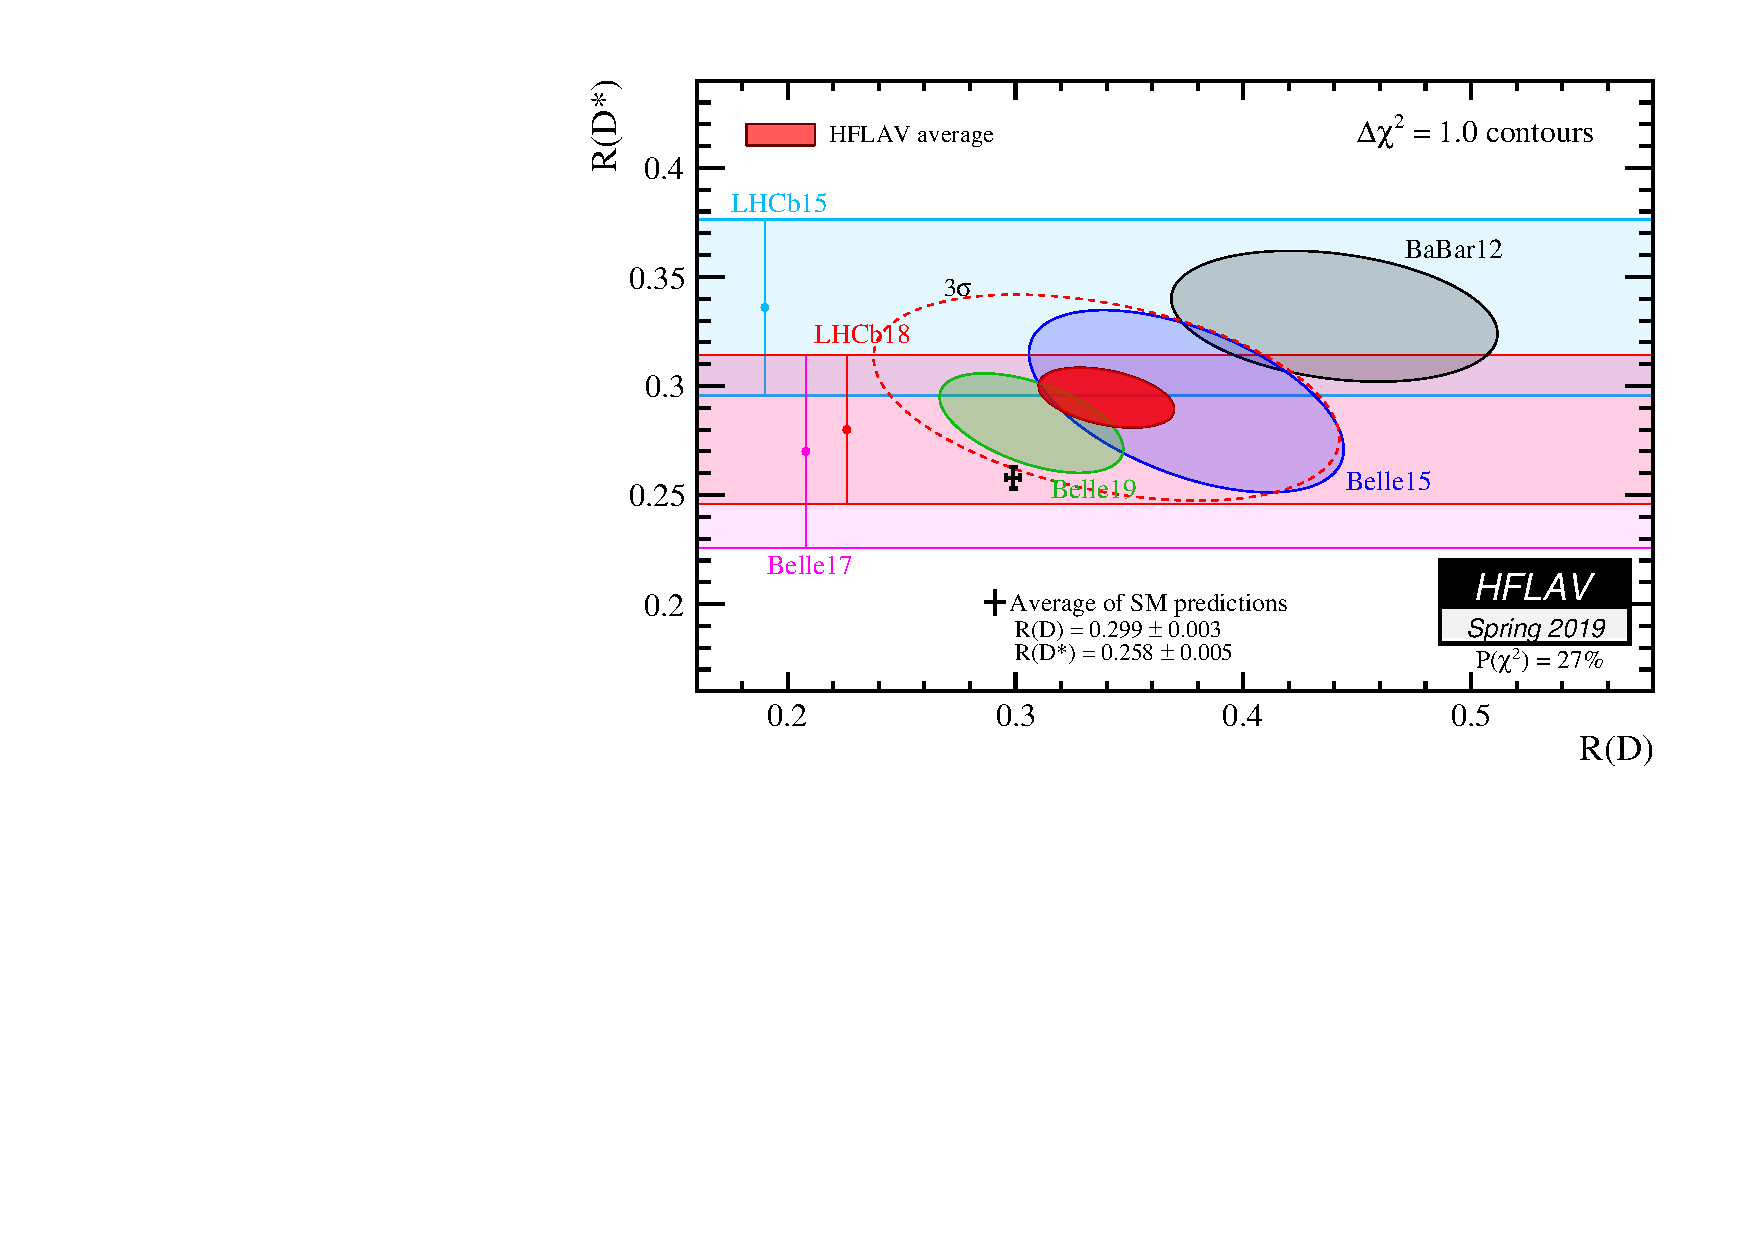
\includegraphics[width=\columnwidth]{figures/rdrds_spring2019.pdf}\\
\colorcite{Y. S. Ahmis \textit{et al.} (HFLAV) arXiv:1909.12524}
        \end{column}
\end{columns}
\end{frame}

\begin{frame}\frametitle{Introduction: Effective Field Theory}
    \setbeamercovered{transparent}
    \def\beamertemplatetransparentcoveredmedium{\setbeamercovered{transparent=50}}
    \beamertemplatetransparentcoveredmedium
    \begin{itemize}
        \item  EFT ``integrates out" heavy degrees of freedom above energy scale $\Lambda$, resulting in operators with dim $> 4$. The short-distance physics is encoded in the Wilson coefficient that multiplies each operator.
              $$\mathcal{L}_\mathrm{EFT} = \mathcal{L}_\mathrm{SM} + \frac{1}{\Lambda}\sum C^{(5)} \mathcal{O}^{(5)} + \frac{1}{\Lambda^2}\sum C^{(6)} \mathcal{O}^{(6)} + \cdots$$
              \vspace{-2mm}
        \item In particular, SMEFT integrates out all NP degrees of freedom.
              \begin{itemize}
                  \item Model-independent description.
                  \item 2499 dimension-6 operators ($\Delta B = \Delta L = 0$).
\item Warsaw basis is the most common choice \colorcite{B. Grzadkowski, Iskrzynski, M. Misiak, J. Rosiek, arXiv:1008.4884}.
                  \item We will consider NP contributions to the following operators:
$$\mathcal{O}_{\ell q(1)}^{ijkl} = (\bar{\ell}_i \gamma_\mu \ell_j)(\bar{q}_k \gamma^\mu  q_l), \qquad \mathcal{O}_{\ell q(3)}^{ijkl} = (\bar{\ell}_i \gamma_\mu \tau^I \ell_j)(\bar{q}_k \gamma^\mu \tau^I q_l).$$
              \end{itemize}
    \end{itemize}
\end{frame}

\begin{frame}\frametitle{Introduction: Effective Field Theory}
\begin{itemize}

\item The scale of $B$ decays is $\mu \approx m_b$. We need to integrate out $t$, $H$, $W$ and $Z$.

\item The Weak Effective Theory (WET) Lagrangian contains
{\scriptsize $$\mathcal{L}_{\text{WET}} \supset -\frac{4 G_F}{\sqrt{2}}V_{cb}\sum_{\ell = e, \mu, \tau} (1 + C_{VL}^\ell) \mathcal{O}_{VL}^\ell + \frac{4G_F}{\sqrt{2}}V_{tb}V_{ts}^*\frac{e^2}{16\pi^2}\sum_{\ell=e,\mu} (C_9^\ell \mathcal{O}_9^\ell  + C_{10}^\ell \mathcal{O}_{10}^\ell) \ ,$$}
{ $$\mathcal{O}_{VL}^\ell = (\bar{c}_L \gamma_\alpha b_L)(\bar{\ell}_L \gamma^\alpha \nu_\ell)\ ,$$ $$\mathcal{O}_9^\ell = (\bar{s}_L \gamma_\alpha b_L)(\bar{\ell} \gamma^\alpha \ell)\ , \qquad \mathcal{O}_{10}^\ell = (\bar{s}_L \gamma_\alpha b_L)(\bar{\ell} \gamma^\alpha \gamma_5 \ell) \ .$$}

\item $\mathcal{O}_{VL}^\ell$ contributes to $R_{D^{(*)}}$ and $\mathcal{O}_9^\ell$, $\mathcal{O}_{10}^\ell$ to $R_{K^{(*)}}$

\item To relate the Wilson coefficients at both scales:
\begin{enumerate}
    \item Run the SMEFT RG equations from $\Lambda$ down to EW scale.
    \item Match the SMEFT operators to the WET operators.
    \item Run the WET RG equations from EW scale down to $m_b$.
\end{enumerate}

\end{itemize}
\end{frame}

\begin{frame}\frametitle{Introduction: Codes}
    Tools used for the global fits (in \texttt{python3}):
    \begin{itemize}
\item \texttt{wilson}: RG evolution and mixing of the Wilson coefficients.\\ \colorcite{J.~Aebischer, J.~Kumar and D.~M.~Straub. arXiv:1804.05033}
\item \texttt{flavio}: Calculation of observables in EFTs and database of experimental measurements. \\ \colorcite{D.~M.~Straub. arXiv:1810.08132}
\item \texttt{smelli}: Global likelihood function:
              {\small$$\Delta \log L = -\frac{1}{2}\Delta\chi^2 = -\frac{1}{2}\sum_{i,j} [\mathcal{O}_i^\mathrm{exp} - \mathcal{O}^\mathrm{th}_i(\vec{C})] (\mathcal{C}^\mathrm{exp}+\mathcal{C}^\mathrm{th}(C))^{-1}_{ij} [\mathcal{O}_j^\mathrm{exp} - \mathcal{O}^\mathrm{th}_j(\vec{C})]\,. $$} % chktex 35
$\mathcal{O}_i^\mathrm{exp}$ is the experimental measurements for the $i$-th observable, and $\mathcal{O}_i^\mathrm{th}$ its SMEFT prediction. $\mathcal{C}_{ij}^\mathrm{exp}$ and $\mathcal{C}^\mathrm{th}(C)$ are the covariance matrices (usually block-diagonal).% chktex 35
\\ \colorcite{J.~Aebischer, J.~Kumar, P.~Stangl and D.~M.~Straub. arXiv:1810.07698}
        \item Custom-made codes, publicly available at \texttt{https://github.com/Jorge-Alda}.
    \end{itemize}
\end{frame}

\begin{frame}[plain] %%% Fit to complex WCs
\begin{block}{\huge Fit to complex Wilson coefficients}
Chapter 5 \\
{\color{red}\textbf{J. Alda}, J. Guasch, S. Peñaranda,\\
\textit{Some Results on Lepton Flavour Universality Violations,}\\
Eur. Phys. J. C 79.7 (2019), p.588, arXiv:1805.03636 [hep-ph].}

\end{block}

\vspace{1.2cm}

\begin{columns}
\begin{column}{0.48\textwidth}
\begin{itemize}
\item Approach
\item Model matching
\item $C_9$ and $C_{10}$
\item Fit to $Z'$ couplings

\end{itemize}
\end{column}
\begin{column}{0.48\textwidth}
\begin{itemize}
\item Fit to $S_3$ couplings
\item Observables
\item Conclusions
\item Update
\end{itemize}
\end{column}
\end{columns}


\end{frame}

\begin{frame}\frametitle{Fit to complex WCs: Approach}
    Common explanation for anomalies in $R_{K^{(*)}}$ and $\Delta M_s$.
    \begin{itemize}
        \item $1.8\ \sigma$ tension with the 2017 theoretical SM prediction for $B_s$ mixing,\\
$\Delta M_S^\mathrm{SM} = 20.01 \pm 1.25\,\mathrm{ps}^{-1}$, \qquad
$\Delta M_S^\mathrm{exp} = 17.757 \pm 0.021
    \,\mathrm{ps}^{-1}$. \\
\colorcite{{L. Di Luzio, M. Kirk, A. Lenz. arXiv:1712.06572}}\\[0.5em]
\item $\mathcal{L}_{\Delta M_S} = -\frac{4 G_f}{\sqrt{2}}
    (V_{tb} V_{ts}^*)^2 C_{bs, \mathrm{NP}}^{LL}
    \mathcal{O}_{bs}^{LL} + \mathrm{h. c.}$
              \begin{itemize}
\item $ \mathcal{O}_{bs}^{LL} = (\bar{s}_L \gamma_\mu b_L)^2$.
\item $\Delta M_S = \Delta M_S^\mathrm{SM} \left|1 + \frac{C_{bs}^{LL} }{R^\mathrm{loop}} \right|$.\\ $\mathrm{Re}(C_{bs}^{LL})< 0$ needed to explain the $\Delta M_S$ anomaly.
\item CP asymmetry: $A_{CP}^\mathrm{mix} (B_s\to J/\psi \phi)= \sin \left[\mathrm{arg}\left(   1 + \frac{C_{bs}^{LL} }{R^\mathrm{loop}} \right) - 2 \beta_s \right] $.
              \end{itemize}
    \end{itemize}

    ~

    We need a model-dependant connection between $R_{K^{(*)}}$ and $\Delta M_s$:
    \begin{itemize}
\item {\color{blue}$Z'$}: $\mathcal{L}_{Z'} = \frac{1}{2} M_{Z'}^2 (Z'_\mu)^2 + (\lambda_{ij}^Q \bar{d}^i_L \gamma^\mu d^j_L + \lambda_{\alpha\beta}^L \bar{e}^\alpha_L \gamma^\mu e_L^\beta )Z'_\mu $.
\item {\color{red}Leptoquarks ($S_3$)}: $\mathcal{L}_{S_3} = -M^2_{S_3} |S_3^a|^2 + y_{i\alpha}^{QL} \bar{q^c}^i (\epsilon \sigma^a) \ell^\alpha S_3^a  + \mathrm{h.c.}$.
    \end{itemize}

\end{frame}

\begin{frame}\frametitle{Fit to complex WCs: Model matching}
Matching to WET coefficients\\ \colorcite{L. Di Luzio, M. Kirk, A. Lenz. arXiv:1712.06572}

% ~

% \begin{columns}
% \begin{column}{0.52\textwidth}
% $$Z'\ \ (\lambda^L_{22} = 1)$$

% {\small $$C_9^\mu = - C_{10}^\mu = \frac{-\pi}{\sqrt{2} G_F \alpha V_{tb} V_{ts}^*}\frac{\lambda^Q_{23}}{M_{Z'}^2}.$$}
% {\small $$C_{bs}^{LL} = \frac{\eta^{LL}}{4\sqrt{2}G_F (V_{tb} V_{ts}^*)^2}\left(\frac{\lambda_{23}^Q}{M_{Z'}}\right)^2.$$}

%         \end{column}
% \begin{column}{0.56\textwidth}
% $$S_3\ \text{leptoquark}$$

% {\small $$C_9^\mu = -C_{10}^\mu = \frac{\pi}{\sqrt{2} G_F \alpha V_{tb} V_{ts}^*} \frac{y^{QL}_{32} y^{QL*}_{22}}{M^2_{S_3}}.$$}
% {\small $$C_{bs}^{LL} = \frac{5\eta^{LL}}{256 \sqrt{2} \pi^2 G_F (V_{tb} V_{ts}^*)^2}\left(\frac{y^{QL}_{3\alpha} y^{QL*}_{2\alpha}}{M_{S_3}}\right)^2.$$}

%         \end{column}
% \end{columns}
\begin{table}
    \centering
    \begin{tabular}{|c|c|}\hline
        {\color{blue}$Z'\ \ (\lambda^L_{22} = 1)$}                 & {\color{red}$S_3\ \text{leptoquark}$} \\\hline
                                                                   &                                       \\
        {\small $C_9^\mu = - C_{10}^\mu = \frac{-\pi}{\sqrt{2} G_F \alpha
        V_{tb} V_{ts}^*}\frac{\lambda^Q_{23}}{M_{Z'}^2}$}          &
        {\small $C_9^\mu = -C_{10}^\mu = \frac{\pi}{\sqrt{2} G_F \alpha V_{tb}
        V_{ts}^*} \frac{y^{QL}_{32} y^{QL*}_{22}}{M^2_{S_3}}$}                                             \\
                                                                   &                                       \\\hline
                                                                   &                                       \\
        {\small $C_{bs}^{LL} = \frac{\eta^{LL}}{4\sqrt{2}G_F (V_{tb}
        V_{ts}^*)^2}\left(\frac{\lambda_{23}^Q}{M_{Z'}}\right)^2$} &
        {\small $C_{bs}^{LL} = \frac{5\eta^{LL}}{256 \sqrt{2} \pi^2 G_F
                        (V_{tb} V_{ts}^*)^2}\left(\frac{y^{QL}_{3\alpha}
                        y^{QL*}_{2\alpha}}{M_{S_3}}\right)^2$}
        \\
                                                                   &                                       \\\hline
    \end{tabular}
\end{table}

\vspace{0.5cm}

A negative value for $C_{bs}^{LL}$ implies a complex value for $C_9^\mu$ and $C_{10}^\mu$ in both models.

\end{frame}

\begin{frame}\frametitle{Fit to complex WCs: $C_9$ and $C_{10}$}

            \begin{figure}
                \centering
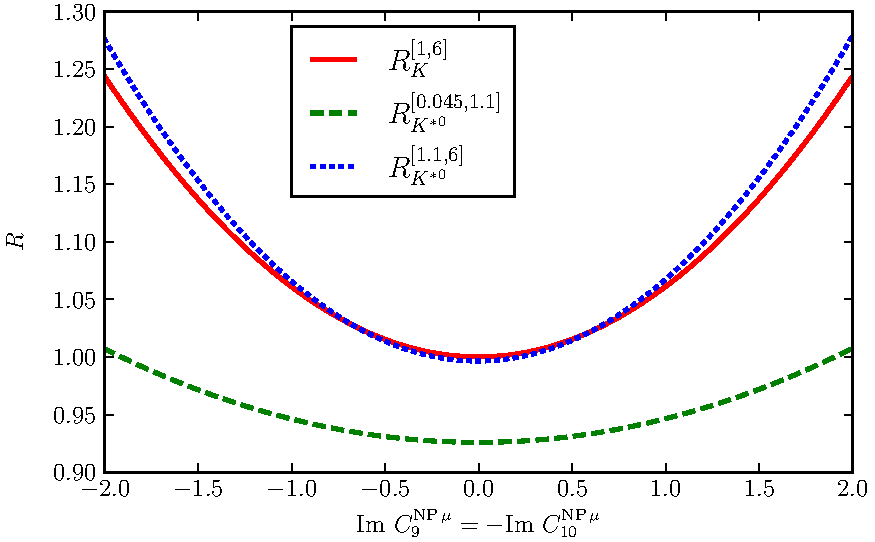
\includegraphics[width=0.7\textwidth]{figures/RK_im.pdf}\\
                Values of $R_{K^{(*)}}$ with imaginary Wilson coefficients.
            \end{figure}


    ~

    \begin{table}
        \centering
        \begin{tabular}{|l|c|c|}\hline
            \textbf{Best fits} & $C_9^\mu=-C_{10}^\mu$ & $\sqrt{\chi^2_\mathrm{SM} - \chi^2_\mathrm{fit}}$ \\\hline
            Real               & $ -0.86$              & $6.0 $                                            \\\hline
            Imaginary          & $-0.005\;i $          & $0.02 $                                           \\\hline
            Complex            & $-1.16\pm 1.14\;i$    & $6.1$                                             \\\hline
        \end{tabular}
    \end{table}
\end{frame}

\begin{frame}\frametitle{Fit to complex WCs: Fit to $Z'$ couplings}
Fit to $R_K$, $R_{K^*}$, $P_4'$, $P_5'$, $\mathcal{B}(B_s \to \mu^+ \mu^-)$, $\Delta M_S$, $A_\mathrm{CP}^\mathrm{mix}(B_s \to J/\psi\, \phi)$.\\[0.3em]

    \begin{figure}
        \begin{columns}
            \begin{column}{0.48\textwidth}
                \centering
{\small Imaginary $Z'$ fit.}\\
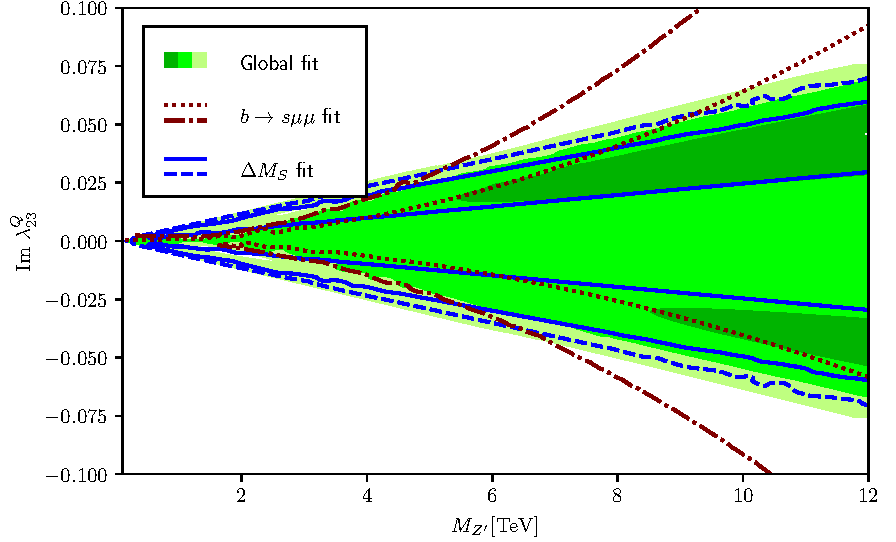
\includegraphics[width=0.9\textwidth]{figures/fitim_Z.pdf}
            \end{column}
            \begin{column}{0.48\textwidth}
\hspace*{1.5cm}{\small Complex $Z'$ fit.}\\
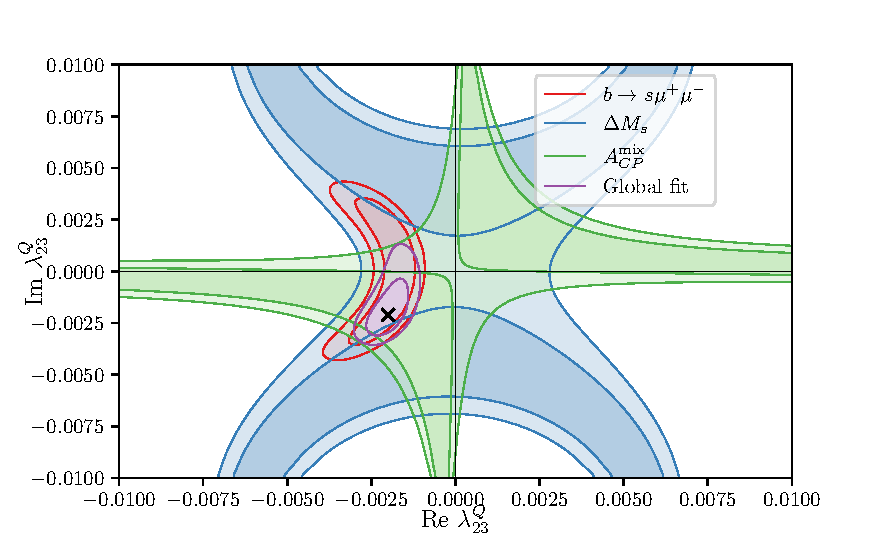
\includegraphics[width=1.0\textwidth]{figures/fitcompl_Z.pdf}
            \end{column}
        \end{columns}
    \end{figure}
    \begin{table}
        \centering
\begin{tabular}{|l|c|c|c|c|}\hline
\textbf{Best fits} & $\lambda^Q_{23}$                                  & $M_{Z'}$
& $\sqrt{\chi^2_\mathrm{SM} - \chi^2_\mathrm{fit}}$ & Pull ($\sigma$)                                      \\\hline
Real               & $-0.002$                                          & $1.31\,\mathrm{TeV}$ & $5.70$ & \alert{$5.39\sigma$} \\\hline
Imaginary          & $\pm 0.047\;i$                                    & $12\,\mathrm{TeV}$   & $1.61$ & \alert{$1.1\sigma$}  \\\hline
Complex            & $-0.0020-0.0021\;i$                               & $1.08\,\mathrm{TeV}$ & $6.05$ & \alert{$5.43\sigma$} \\\hline
        \end{tabular}
    \end{table}

    The better fit is provided by complex couplings.
\end{frame}

\begin{frame}\frametitle{Fit to complex WCs: Fit to $S_3$ couplings}
Fit to $R_K$, $R_{K^*}$, $P_4'$, $P_5'$, $\mathcal{B}(B_s \to \mu^+ \mu^-)$, $\Delta M_S$, $A_\mathrm{CP}^\mathrm{mix}(B_s \to J/\psi\, \phi)$.\\[0.3em]

    \begin{figure}
        \begin{columns}
            \begin{column}{0.48\textwidth}
                \centering
{\small Imaginary $S_3$ fit.}\\
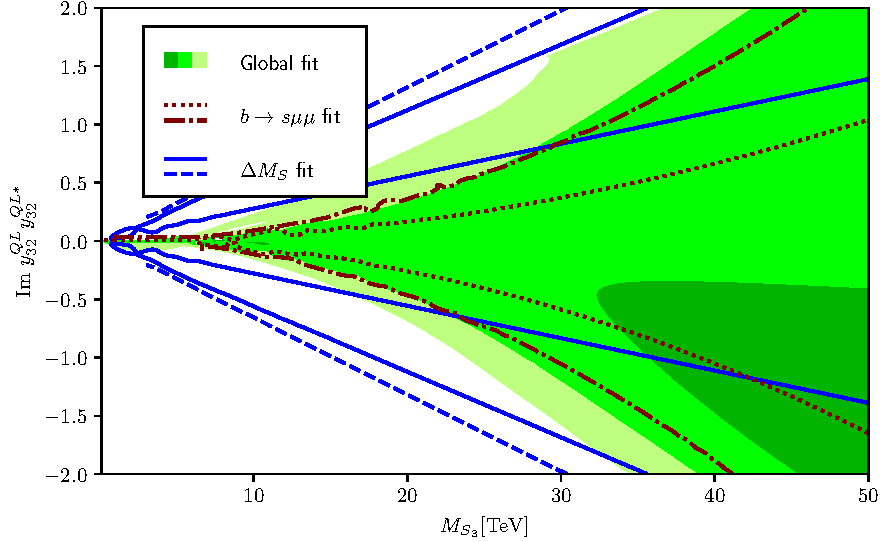
\includegraphics[width=0.9\textwidth]{figures/fitim_LQ.pdf}
            \end{column}
            \begin{column}{0.48\textwidth}
\hspace*{1.5cm}{\small Complex $S_3$ fit.}\\
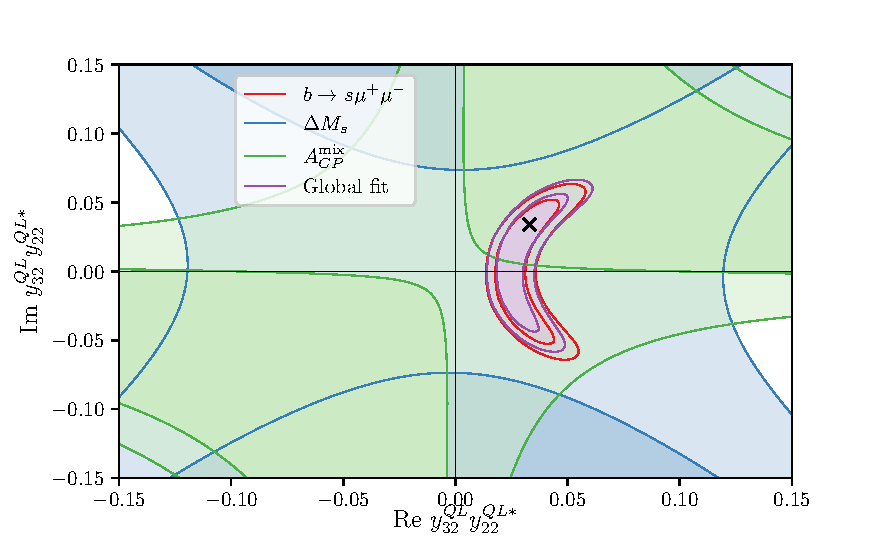
\includegraphics[width=1.0\textwidth]{figures/fitcompl_LQ.pdf}

            \end{column}
        \end{columns}
    \end{figure}

    \begin{table}
        \centering
\begin{tabular}{|l|c|c|c|c|}\hline
\textbf{Best fits}   & $y^{QL}_{32} y^{QL*}_{22}$                        & $M_{S_3}$
& $\sqrt{\chi^2_\mathrm{SM} - \chi^2_\mathrm{fit}}$ & Pull ($\sigma$)      \\\hline
Real                 & $ 0.04 $                                          &
$5.19\,\mathrm{TeV}$ & $5.82$                                            & \alert{$5.47\sigma$} \\\hline
Imaginary            & $-1.67\;i$                                        &
$50\,\mathrm{TeV}$   & $1.15$                                            & \alert{$0.6\sigma$}  \\\hline
Complex              & $0.033+0.034\;i$                                  &
$4.10\,\mathrm{TeV}$ & $5.90$                                            & \alert{$5.27\sigma$} \\\hline
        \end{tabular}
    \end{table}

Complex couplings provide a similar fit compared to real case.

\end{frame}

\begin{frame}\frametitle{Fit to complex WCs: Observables}
    \begin{figure}
        \begin{columns}
            \begin{column}{0.48\textwidth}
                \centering
$$R_{K^{(*)}}$$
                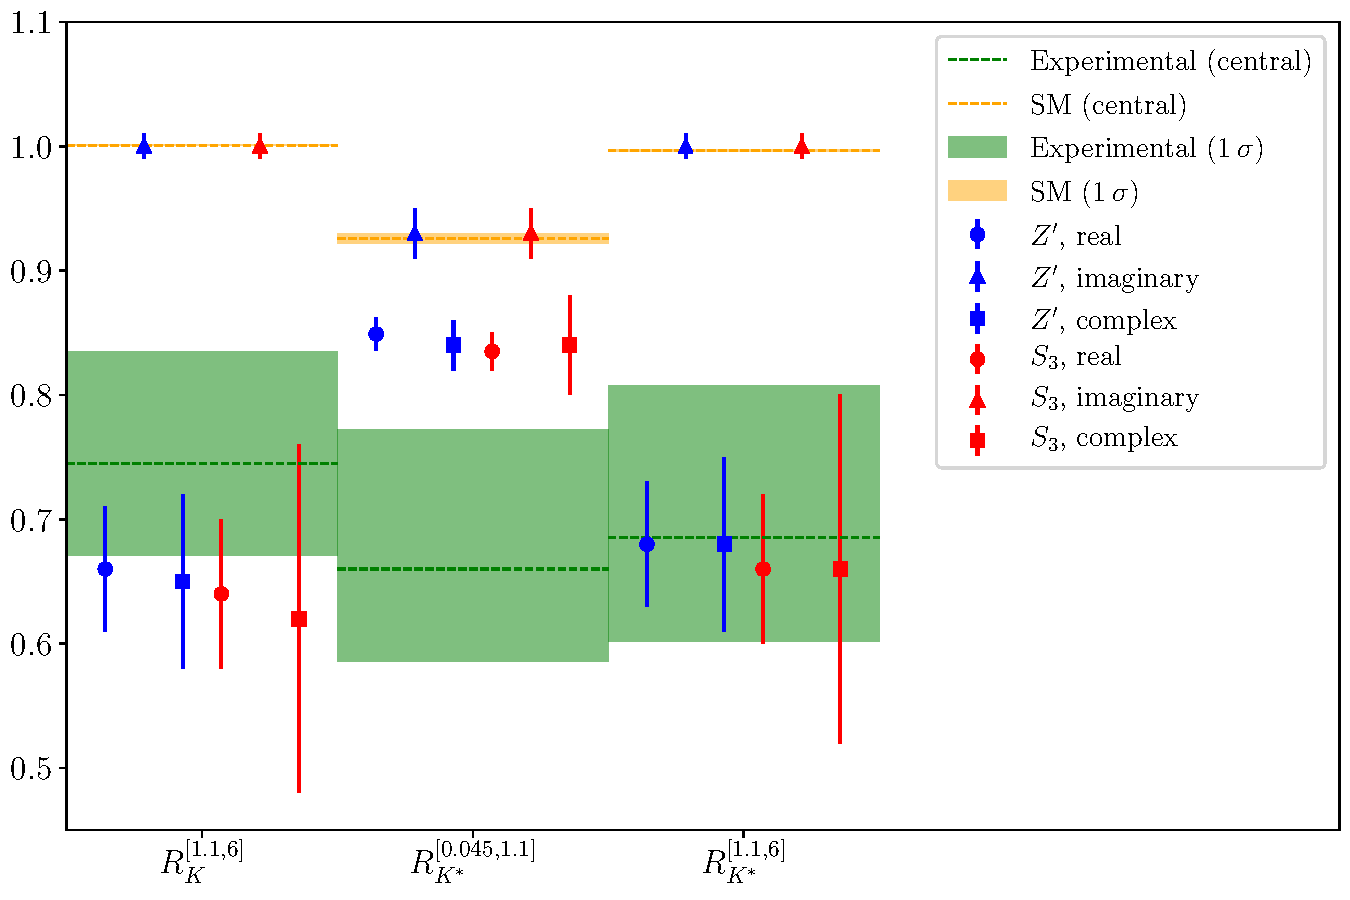
\includegraphics[width = 0.8\textwidth]{figures/errorplot_RKmodels.pdf}
            \end{column}
            \begin{column}{0.48\textwidth}
$1\sigma$ intervals for observables in the
    {\color{blue}$Z'$} and {\color{red} LQ} fits, compared
to the {\color{green} experimental values} and
    {\color{orange} SM predictions}.
            \end{column}
        \end{columns}
    \end{figure}
\vspace{-0.2cm}
    \begin{figure}
        \begin{columns}
            \begin{column}{0.48\textwidth}
                \centering
$$\Delta M_S$$
                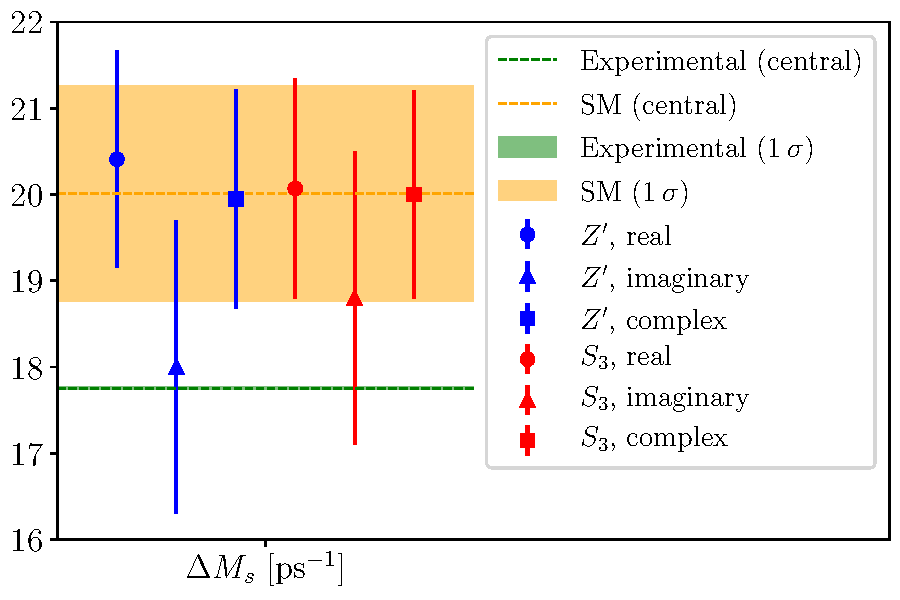
\includegraphics[width = 0.8\textwidth]{figures/errorplot_DMsmodels.pdf}
            \end{column}
            \begin{column}{0.48\textwidth}
                \centering
$$A_{CP}^\mathrm{mix}$$
                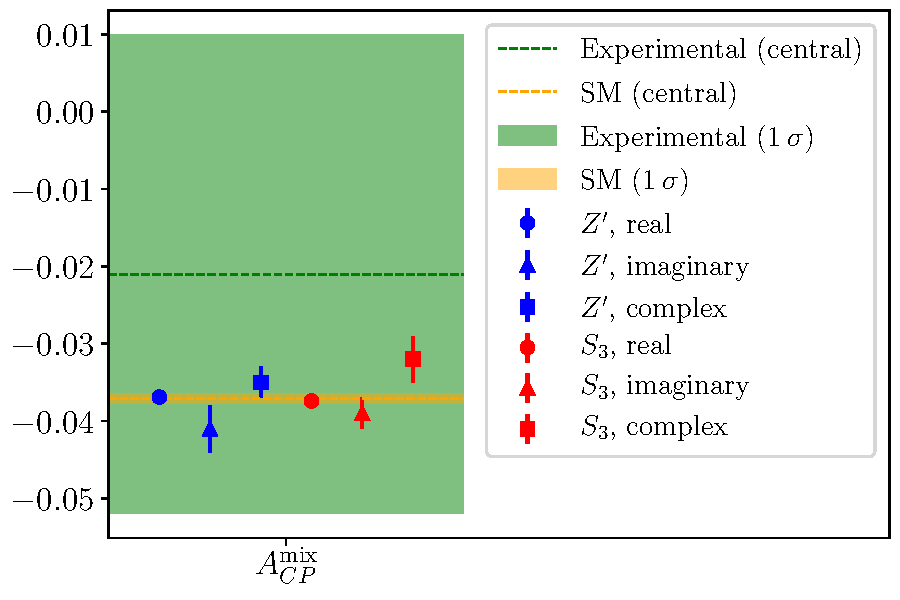
\includegraphics[width = 0.8\textwidth]{figures/errorplot_ACPmodels.pdf}
            \end{column}
        \end{columns}
    \end{figure}
\end{frame}

\begin{frame}\frametitle{Fit to complex WCs: Conclusions}
    \begin{itemize}
        \item Hints of New Physics violating Lepton Flavour Universality in the $B$ sector.
        \item Characterization using EFT and model building.
        \item Real Wilson coefficients cannot explain the $B_S$ mixing anomaly; imaginary Wilson coefficients cannot explain the $R_{K^{(*)}}$ anomaly.
        \item Complex couplings offer a slightly better global fit.

    \end{itemize}

\end{frame}

\begin{frame}\frametitle{Fit to complex WCs: Update}
    \begin{itemize}
\item The SM prediction for $\Delta M_S$ was updated in 2019 to $\Delta M_S = (18.4^{+0.7}_{-1.2}) \mathrm{ps}^{-1}$, compatible with experiment.\\ \colorcite{L. Di Luzio, M. Kirk, A. Lenz, and T. Rauh, arXiv:1909.11087}
        \item Therefore, imaginary or complex WC are no longer necessary. In the following fits we only consider real parameters.
        \item After the 2019 and 2021 $R_K$ measurements by LHCb, our results are not compatible with experimental data.
    \end{itemize}

    \begin{center}
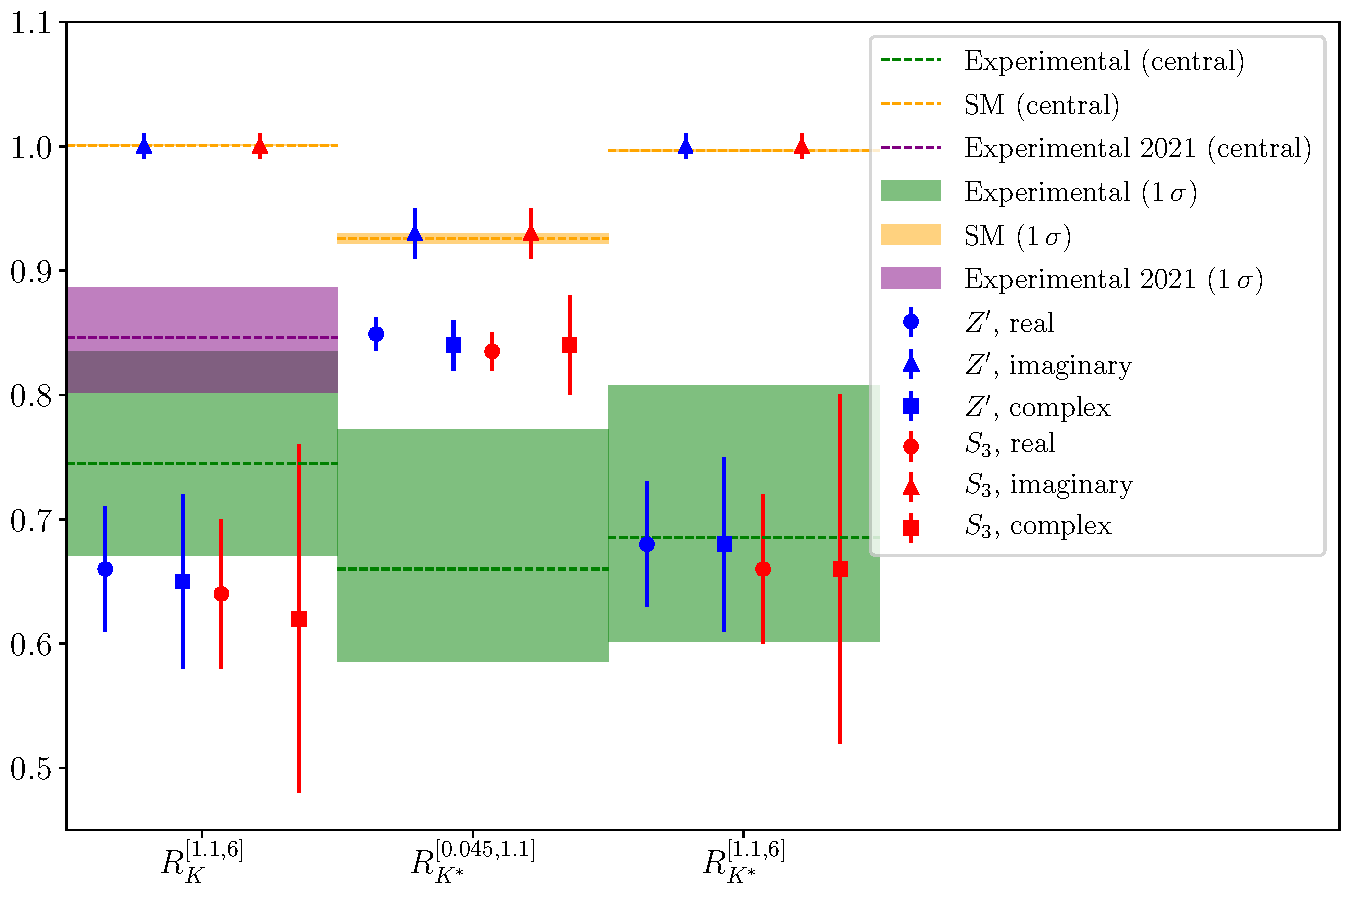
\includegraphics[width=0.54\textwidth]{figures/errorplot_RK2021.pdf}
    \end{center}

\end{frame}

\begin{frame}[plain] %%% SMEFT Fit
\begin{block}{\huge Fit to SMEFT coefficients\\ and future prospects}
    Chapter 6\\
    {\color{red} \textbf{J. Alda}, J. Guasch, S. Peñaranda,\\
    \textit{Anomalies in B meson decays: A phenomenological approach,}\\
    Eur. Phys. J. Plus 137 (2022), p.217, arXiv:2012.14799 [hep-ph]}
\end{block}

\vspace{1.3cm}

\begin{columns}
\begin{column}{0.48\textwidth}
\begin{itemize}
\item Operators and observables
\item Global fits
\item Observables
%\item Hessian approximation

\end{itemize}
\end{column}
\begin{column}{0.48\textwidth}
\begin{itemize}
% \item Electron colliders
\item Hessian approximation
\item Improved EW prospects
\item Conclusions
\end{itemize}
\end{column}
\end{columns}

\end{frame}

\begin{frame}\frametitle{SMEFT Fit: Operators and observables}
    In this fit, we will consider the following SMEFT operators
    $$\mathcal{O}^i_{\ell q (1)} = (\overline{\ell}_i \gamma_\mu \ell_i)(\overline{q}_3 \gamma^\mu q_3), \qquad
        \mathcal{O}^i_{\ell q (3)} = (\overline{\ell}_i \gamma_\mu \tau^I \ell_i)(\overline{q}_3 \gamma^\mu \tau^I q_3),$$
    \begin{itemize}
        \item Constrains from $\mathrm{BR}(B\to K^{(*)} \nu\overline{\nu})$ impose
              $$C_{\ell q (1)}^i = C_{\ell q (3)}^i \equiv C_{\ell q}^i.\qquad\qquad$$
        \item We obtained the running from the SMEFT operators at $\Lambda =$ 1 TeV down to $\mu = m_b$ using the RGE:
              {\scriptsize\begin{align*}
C_9^{\mathrm{NP}\ e, \mu} = -0.583 \, C_{\ell
        q(1)}^{e, \mu} - 0.596 \, C_{\ell q(3)}^{e, \mu}\ , & \qquad C_{10}^{\mathrm{NP}\ e, \mu} = 0.588 \, C_{\ell q(1)}^{e,
        \mu} + 0.591 \, C_{\ell q(3)}^{e, \mu}\ , \nonumber                                                                    \\
C_{VL}^{e, \mu} = 0.0012 \, C_{\ell q(1)}^{e, \mu} -
0.0644\, C_{\ell q(3)}^{e, \mu}\ ,                  & \qquad
C_{VL}^\tau =  -0.0598\,  C_{\ell  q(3)}^\tau\   .
                  \label{eq:running}
              \end{align*}}
        \item RG causes mixing to other physical sectors (e.g. electroweak tests) $\Longrightarrow$ We need global fits: $B$-physics\tikzmark{Bphys}, EW\tikzmark{EW}, $\beta$ decays, etc.
    \end{itemize}
    \mycallout<2>{Bphys}{$R_{K^{(*)}}$ and differential observables, $R_{D^{(*)}}$, $B_{(s)}\to\mu^+\mu^-$, $B\to K^{(*)} \nu\overline{\nu}$}
    \anothercallout<2>{EW}{$\Gamma_Z$, $M_W$, $A_e$, $A_\mu$, $A_\tau$, $A_b$, $A_c$, $R_e$, $R_\mu$, $R_\tau$, $R_b$, $R_c$, $A^\mathrm{FB}$, $\sigma_0^\mathrm{had}$}

\end{frame}

\begin{frame}\frametitle{SMEFT Fit: Global fits}
    \begin{center}
{\footnotesize Fit to $C_{\ell q}^e$ and $C_{\ell q}^\mu$ $\qquad\qquad\qquad   \qquad$ Fit to $C_{\ell q}^e = -C_{\ell q}^\mu$ and $C_{\ell q}^\tau$}
        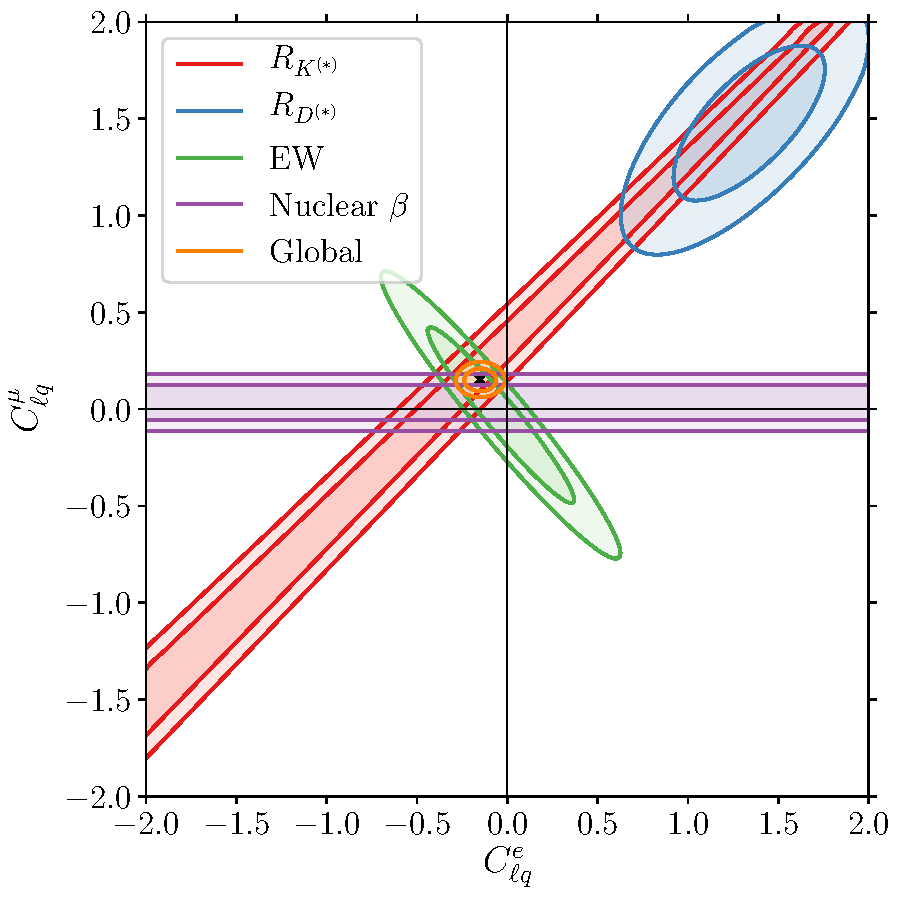
\includegraphics[width=0.4\textwidth]{figures/scIV_beta.pdf} $\qquad$
        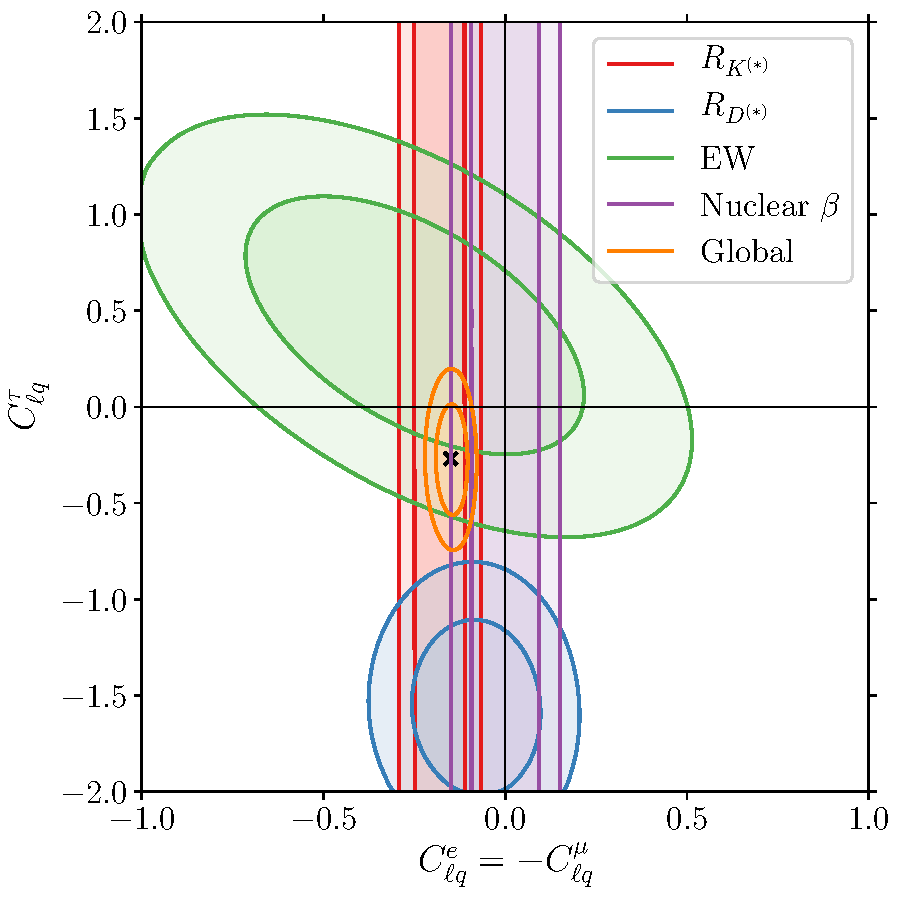
\includegraphics[width=0.4\textwidth]{figures/scXI_beta.pdf}
    \end{center}
    \begin{itemize}
        \item $C_{\ell q}^\mu - C_{\ell q}^e$ describes violations of lepton universality, fit dominated by $R_{K^{(*)}}$ and $R_{D^{(*)}}$ observables. Large deviations from SM.
        \item $C_{\ell q}^\mu + C_{\ell q}^e$ describes flavour-universal contributions, fit dominated by EW observables. Compatible with SM.
        \item $\beta$ decays are sensitive to deviations in $C_{\ell q}^\mu$.
        \item $C_{\ell q}^\tau$ uncorrelated with the other operators. Compatible with SM (but large uncertainties).
    \end{itemize}

\end{frame}

\begin{frame}\frametitle{SMEFT Fit: Observables}

We consider different scenarios for the SMEFT coefficients.\\[0.3em]
The most relevant are: \vspace{-0.5cm}
{\scriptsize
\hspace*{-2em}%
\begin{minipage}[t][2.5cm][t]{\textwidth}
\begin{columns}[onlytextwidth]
\begin{column}{0.52\textwidth}
\begin{itemize}
\item Scenario IV: Fit to $C_{\ell q}^e$, $C_{\ell q}^\mu\ [4.73\,\sigma]$.
\item Scenario VII: Fit to $C_{\ell q}^e$, $C_{\ell q}^\mu$, $C_{\ell q}^\tau\ [4.97\,\sigma]$.
\end{itemize}
\end{column}
\begin{column}{0.58\textwidth}
\begin{itemize}
\item Scenario IX: Fit to $C_{\ell q}^e = C_{\ell q}^\tau = - C_{\ell q}^\mu\ [5.27\,\sigma]$.
\item Scenario X: Fit to $C_{\ell q}^e =  - C_{\ell q}^\mu\ [4.94\,\sigma]$.
\item Scenario XI: Fit to $C_{\ell q}^e = - C_{\ell q}^\mu$, $C_{\ell q}^\tau\ [4.94\,\sigma]$.
\end{itemize}
\end{column}
\end{columns}
\end{minipage}
}\vspace*{-1.0cm}
    \begin{figure}\begin{center}
{\small{$$\qquad R_{K^{(*)}}\qquad\qquad\qquad\qquad\qquad\qquad\qquad R_{D^{(*)}}$$}}
\resizebox{0.50\textwidth}{!}{%% Creator: Matplotlib, PGF backend
%%
%% To include the figure in your LaTeX document, write
%%   \input{<filename>.pgf}
%%
%% Make sure the required packages are loaded in your preamble
%%   \usepackage{pgf}
%%
%% and, on pdftex
%%   \usepackage[utf8]{inputenc}\DeclareUnicodeCharacter{2212}{-}
%%
%% or, on luatex and xetex
%%   \usepackage{unicode-math}
%%
%% Figures using additional raster images can only be included by \input if
%% they are in the same directory as the main LaTeX file. For loading figures
%% from other directories you can use the `import` package
%%   \usepackage{import}
%%
%% and then include the figures with
%%   \import{<path to file>}{<filename>.pgf}
%%
%% Matplotlib used the following preamble
%%
\begingroup%
\makeatletter%
\begin{pgfpicture}%
\pgfpathrectangle{\pgfpointorigin}{\pgfqpoint{8.000000in}{5.000000in}}%
\pgfusepath{use as bounding box, clip}%
\begin{pgfscope}%
\pgfsetbuttcap%
\pgfsetmiterjoin%
\definecolor{currentfill}{rgb}{1.000000,1.000000,1.000000}%
\pgfsetfillcolor{currentfill}%
\pgfsetlinewidth{0.000000pt}%
\definecolor{currentstroke}{rgb}{1.000000,1.000000,1.000000}%
\pgfsetstrokecolor{currentstroke}%
\pgfsetdash{}{0pt}%
\pgfpathmoveto{\pgfqpoint{0.000000in}{0.000000in}}%
\pgfpathlineto{\pgfqpoint{8.000000in}{0.000000in}}%
\pgfpathlineto{\pgfqpoint{8.000000in}{5.000000in}}%
\pgfpathlineto{\pgfqpoint{0.000000in}{5.000000in}}%
\pgfpathclose%
\pgfusepath{fill}%
\end{pgfscope}%
\begin{pgfscope}%
\pgfsetbuttcap%
\pgfsetmiterjoin%
\definecolor{currentfill}{rgb}{1.000000,1.000000,1.000000}%
\pgfsetfillcolor{currentfill}%
\pgfsetlinewidth{0.000000pt}%
\definecolor{currentstroke}{rgb}{0.000000,0.000000,0.000000}%
\pgfsetstrokecolor{currentstroke}%
\pgfsetstrokeopacity{0.000000}%
\pgfsetdash{}{0pt}%
\pgfpathmoveto{\pgfqpoint{0.443660in}{0.465794in}}%
\pgfpathlineto{\pgfqpoint{5.806218in}{0.465794in}}%
\pgfpathlineto{\pgfqpoint{5.806218in}{4.930556in}}%
\pgfpathlineto{\pgfqpoint{0.443660in}{4.930556in}}%
\pgfpathclose%
\pgfusepath{fill}%
\end{pgfscope}%
\begin{pgfscope}%
\pgfpathrectangle{\pgfqpoint{0.443660in}{0.465794in}}{\pgfqpoint{5.362558in}{4.464761in}}%
\pgfusepath{clip}%
\pgfsetbuttcap%
\pgfsetmiterjoin%
\definecolor{currentfill}{rgb}{1.000000,0.647059,0.000000}%
\pgfsetfillcolor{currentfill}%
\pgfsetfillopacity{0.500000}%
\pgfsetlinewidth{0.000000pt}%
\definecolor{currentstroke}{rgb}{1.000000,0.647059,0.000000}%
\pgfsetstrokecolor{currentstroke}%
\pgfsetstrokeopacity{0.500000}%
\pgfsetdash{}{0pt}%
\pgfpathmoveto{\pgfqpoint{0.533036in}{4.673425in}}%
\pgfpathlineto{\pgfqpoint{2.141803in}{4.673425in}}%
\pgfpathlineto{\pgfqpoint{2.141803in}{4.727612in}}%
\pgfpathlineto{\pgfqpoint{0.533036in}{4.727612in}}%
\pgfpathclose%
\pgfusepath{fill}%
\end{pgfscope}%
\begin{pgfscope}%
\pgfpathrectangle{\pgfqpoint{0.443660in}{0.465794in}}{\pgfqpoint{5.362558in}{4.464761in}}%
\pgfusepath{clip}%
\pgfsetbuttcap%
\pgfsetmiterjoin%
\definecolor{currentfill}{rgb}{0.000000,0.501961,0.000000}%
\pgfsetfillcolor{currentfill}%
\pgfsetfillopacity{0.500000}%
\pgfsetlinewidth{0.000000pt}%
\definecolor{currentstroke}{rgb}{0.000000,0.501961,0.000000}%
\pgfsetstrokecolor{currentstroke}%
\pgfsetstrokeopacity{0.500000}%
\pgfsetdash{}{0pt}%
\pgfpathmoveto{\pgfqpoint{0.533036in}{3.000524in}}%
\pgfpathlineto{\pgfqpoint{2.141803in}{3.000524in}}%
\pgfpathlineto{\pgfqpoint{2.141803in}{3.638115in}}%
\pgfpathlineto{\pgfqpoint{0.533036in}{3.638115in}}%
\pgfpathclose%
\pgfusepath{fill}%
\end{pgfscope}%
\begin{pgfscope}%
\pgfpathrectangle{\pgfqpoint{0.443660in}{0.465794in}}{\pgfqpoint{5.362558in}{4.464761in}}%
\pgfusepath{clip}%
\pgfsetbuttcap%
\pgfsetmiterjoin%
\definecolor{currentfill}{rgb}{0.000000,0.501961,0.000000}%
\pgfsetfillcolor{currentfill}%
\pgfsetfillopacity{0.500000}%
\pgfsetlinewidth{0.000000pt}%
\definecolor{currentstroke}{rgb}{0.000000,0.501961,0.000000}%
\pgfsetstrokecolor{currentstroke}%
\pgfsetstrokeopacity{0.500000}%
\pgfsetdash{}{0pt}%
\pgfpathmoveto{\pgfqpoint{2.320555in}{0.668738in}}%
\pgfpathlineto{\pgfqpoint{3.929322in}{0.668738in}}%
\pgfpathlineto{\pgfqpoint{3.929322in}{2.364572in}}%
\pgfpathlineto{\pgfqpoint{2.320555in}{2.364572in}}%
\pgfpathclose%
\pgfusepath{fill}%
\end{pgfscope}%
\begin{pgfscope}%
\pgfpathrectangle{\pgfqpoint{0.443660in}{0.465794in}}{\pgfqpoint{5.362558in}{4.464761in}}%
\pgfusepath{clip}%
\pgfsetbuttcap%
\pgfsetmiterjoin%
\definecolor{currentfill}{rgb}{1.000000,0.647059,0.000000}%
\pgfsetfillcolor{currentfill}%
\pgfsetfillopacity{0.500000}%
\pgfsetlinewidth{0.000000pt}%
\definecolor{currentstroke}{rgb}{1.000000,0.647059,0.000000}%
\pgfsetstrokecolor{currentstroke}%
\pgfsetstrokeopacity{0.500000}%
\pgfsetdash{}{0pt}%
\pgfpathmoveto{\pgfqpoint{2.320555in}{3.974583in}}%
\pgfpathlineto{\pgfqpoint{3.929322in}{3.974583in}}%
\pgfpathlineto{\pgfqpoint{3.929322in}{4.053859in}}%
\pgfpathlineto{\pgfqpoint{2.320555in}{4.053859in}}%
\pgfpathclose%
\pgfusepath{fill}%
\end{pgfscope}%
\begin{pgfscope}%
\pgfpathrectangle{\pgfqpoint{0.443660in}{0.465794in}}{\pgfqpoint{5.362558in}{4.464761in}}%
\pgfusepath{clip}%
\pgfsetbuttcap%
\pgfsetmiterjoin%
\definecolor{currentfill}{rgb}{0.000000,0.501961,0.000000}%
\pgfsetfillcolor{currentfill}%
\pgfsetfillopacity{0.500000}%
\pgfsetlinewidth{0.000000pt}%
\definecolor{currentstroke}{rgb}{0.000000,0.501961,0.000000}%
\pgfsetstrokecolor{currentstroke}%
\pgfsetstrokeopacity{0.500000}%
\pgfsetdash{}{0pt}%
\pgfpathmoveto{\pgfqpoint{4.108074in}{0.865484in}}%
\pgfpathlineto{\pgfqpoint{5.716842in}{0.865484in}}%
\pgfpathlineto{\pgfqpoint{5.716842in}{2.694700in}}%
\pgfpathlineto{\pgfqpoint{4.108074in}{2.694700in}}%
\pgfpathclose%
\pgfusepath{fill}%
\end{pgfscope}%
\begin{pgfscope}%
\pgfpathrectangle{\pgfqpoint{0.443660in}{0.465794in}}{\pgfqpoint{5.362558in}{4.464761in}}%
\pgfusepath{clip}%
\pgfsetbuttcap%
\pgfsetmiterjoin%
\definecolor{currentfill}{rgb}{1.000000,0.647059,0.000000}%
\pgfsetfillcolor{currentfill}%
\pgfsetfillopacity{0.500000}%
\pgfsetlinewidth{0.000000pt}%
\definecolor{currentstroke}{rgb}{1.000000,0.647059,0.000000}%
\pgfsetstrokecolor{currentstroke}%
\pgfsetstrokeopacity{0.500000}%
\pgfsetdash{}{0pt}%
\pgfpathmoveto{\pgfqpoint{4.108074in}{4.616859in}}%
\pgfpathlineto{\pgfqpoint{5.716842in}{4.616859in}}%
\pgfpathlineto{\pgfqpoint{5.716842in}{4.704857in}}%
\pgfpathlineto{\pgfqpoint{4.108074in}{4.704857in}}%
\pgfpathclose%
\pgfusepath{fill}%
\end{pgfscope}%
\begin{pgfscope}%
\pgfsetbuttcap%
\pgfsetroundjoin%
\definecolor{currentfill}{rgb}{0.000000,0.000000,0.000000}%
\pgfsetfillcolor{currentfill}%
\pgfsetlinewidth{0.803000pt}%
\definecolor{currentstroke}{rgb}{0.000000,0.000000,0.000000}%
\pgfsetstrokecolor{currentstroke}%
\pgfsetdash{}{0pt}%
\pgfsys@defobject{currentmarker}{\pgfqpoint{0.000000in}{-0.048611in}}{\pgfqpoint{0.000000in}{0.000000in}}{%
\pgfpathmoveto{\pgfqpoint{0.000000in}{0.000000in}}%
\pgfpathlineto{\pgfqpoint{0.000000in}{-0.048611in}}%
\pgfusepath{stroke,fill}%
}%
\begin{pgfscope}%
\pgfsys@transformshift{1.337420in}{0.465794in}%
\pgfsys@useobject{currentmarker}{}%
\end{pgfscope}%
\end{pgfscope}%
\begin{pgfscope}%
\definecolor{textcolor}{rgb}{0.000000,0.000000,0.000000}%
\pgfsetstrokecolor{textcolor}%
\pgfsetfillcolor{textcolor}%
\pgftext[x=1.337420in,y=0.368572in,,top]{\color{textcolor}\rmfamily\fontsize{16.000000}{19.200000}\selectfont \(\displaystyle R_{K^+}^{[1.1,6]}\)}%
\end{pgfscope}%
\begin{pgfscope}%
\pgfsetbuttcap%
\pgfsetroundjoin%
\definecolor{currentfill}{rgb}{0.000000,0.000000,0.000000}%
\pgfsetfillcolor{currentfill}%
\pgfsetlinewidth{0.803000pt}%
\definecolor{currentstroke}{rgb}{0.000000,0.000000,0.000000}%
\pgfsetstrokecolor{currentstroke}%
\pgfsetdash{}{0pt}%
\pgfsys@defobject{currentmarker}{\pgfqpoint{0.000000in}{-0.048611in}}{\pgfqpoint{0.000000in}{0.000000in}}{%
\pgfpathmoveto{\pgfqpoint{0.000000in}{0.000000in}}%
\pgfpathlineto{\pgfqpoint{0.000000in}{-0.048611in}}%
\pgfusepath{stroke,fill}%
}%
\begin{pgfscope}%
\pgfsys@transformshift{3.124939in}{0.465794in}%
\pgfsys@useobject{currentmarker}{}%
\end{pgfscope}%
\end{pgfscope}%
\begin{pgfscope}%
\definecolor{textcolor}{rgb}{0.000000,0.000000,0.000000}%
\pgfsetstrokecolor{textcolor}%
\pgfsetfillcolor{textcolor}%
\pgftext[x=3.124939in,y=0.368572in,,top]{\color{textcolor}\rmfamily\fontsize{16.000000}{19.200000}\selectfont \(\displaystyle R_{K^*0}^{[0.045, 1.1]}\)}%
\end{pgfscope}%
\begin{pgfscope}%
\pgfsetbuttcap%
\pgfsetroundjoin%
\definecolor{currentfill}{rgb}{0.000000,0.000000,0.000000}%
\pgfsetfillcolor{currentfill}%
\pgfsetlinewidth{0.803000pt}%
\definecolor{currentstroke}{rgb}{0.000000,0.000000,0.000000}%
\pgfsetstrokecolor{currentstroke}%
\pgfsetdash{}{0pt}%
\pgfsys@defobject{currentmarker}{\pgfqpoint{0.000000in}{-0.048611in}}{\pgfqpoint{0.000000in}{0.000000in}}{%
\pgfpathmoveto{\pgfqpoint{0.000000in}{0.000000in}}%
\pgfpathlineto{\pgfqpoint{0.000000in}{-0.048611in}}%
\pgfusepath{stroke,fill}%
}%
\begin{pgfscope}%
\pgfsys@transformshift{4.912458in}{0.465794in}%
\pgfsys@useobject{currentmarker}{}%
\end{pgfscope}%
\end{pgfscope}%
\begin{pgfscope}%
\definecolor{textcolor}{rgb}{0.000000,0.000000,0.000000}%
\pgfsetstrokecolor{textcolor}%
\pgfsetfillcolor{textcolor}%
\pgftext[x=4.912458in,y=0.368572in,,top]{\color{textcolor}\rmfamily\fontsize{16.000000}{19.200000}\selectfont \(\displaystyle R_{K^*0}^{[1.1, 6]}\)}%
\end{pgfscope}%
\begin{pgfscope}%
\pgfsetbuttcap%
\pgfsetroundjoin%
\definecolor{currentfill}{rgb}{0.000000,0.000000,0.000000}%
\pgfsetfillcolor{currentfill}%
\pgfsetlinewidth{0.803000pt}%
\definecolor{currentstroke}{rgb}{0.000000,0.000000,0.000000}%
\pgfsetstrokecolor{currentstroke}%
\pgfsetdash{}{0pt}%
\pgfsys@defobject{currentmarker}{\pgfqpoint{-0.048611in}{0.000000in}}{\pgfqpoint{0.000000in}{0.000000in}}{%
\pgfpathmoveto{\pgfqpoint{0.000000in}{0.000000in}}%
\pgfpathlineto{\pgfqpoint{-0.048611in}{0.000000in}}%
\pgfusepath{stroke,fill}%
}%
\begin{pgfscope}%
\pgfsys@transformshift{0.443660in}{1.036270in}%
\pgfsys@useobject{currentmarker}{}%
\end{pgfscope}%
\end{pgfscope}%
\begin{pgfscope}%
\definecolor{textcolor}{rgb}{0.000000,0.000000,0.000000}%
\pgfsetstrokecolor{textcolor}%
\pgfsetfillcolor{textcolor}%
\pgftext[x=0.061024in, y=0.952937in, left, base]{\color{textcolor}\rmfamily\fontsize{16.000000}{19.200000}\selectfont \(\displaystyle 0.6\)}%
\end{pgfscope}%
\begin{pgfscope}%
\pgfsetbuttcap%
\pgfsetroundjoin%
\definecolor{currentfill}{rgb}{0.000000,0.000000,0.000000}%
\pgfsetfillcolor{currentfill}%
\pgfsetlinewidth{0.803000pt}%
\definecolor{currentstroke}{rgb}{0.000000,0.000000,0.000000}%
\pgfsetstrokecolor{currentstroke}%
\pgfsetdash{}{0pt}%
\pgfsys@defobject{currentmarker}{\pgfqpoint{-0.048611in}{0.000000in}}{\pgfqpoint{0.000000in}{0.000000in}}{%
\pgfpathmoveto{\pgfqpoint{0.000000in}{0.000000in}}%
\pgfpathlineto{\pgfqpoint{-0.048611in}{0.000000in}}%
\pgfusepath{stroke,fill}%
}%
\begin{pgfscope}%
\pgfsys@transformshift{0.443660in}{1.950551in}%
\pgfsys@useobject{currentmarker}{}%
\end{pgfscope}%
\end{pgfscope}%
\begin{pgfscope}%
\definecolor{textcolor}{rgb}{0.000000,0.000000,0.000000}%
\pgfsetstrokecolor{textcolor}%
\pgfsetfillcolor{textcolor}%
\pgftext[x=0.061024in, y=1.867218in, left, base]{\color{textcolor}\rmfamily\fontsize{16.000000}{19.200000}\selectfont \(\displaystyle 0.7\)}%
\end{pgfscope}%
\begin{pgfscope}%
\pgfsetbuttcap%
\pgfsetroundjoin%
\definecolor{currentfill}{rgb}{0.000000,0.000000,0.000000}%
\pgfsetfillcolor{currentfill}%
\pgfsetlinewidth{0.803000pt}%
\definecolor{currentstroke}{rgb}{0.000000,0.000000,0.000000}%
\pgfsetstrokecolor{currentstroke}%
\pgfsetdash{}{0pt}%
\pgfsys@defobject{currentmarker}{\pgfqpoint{-0.048611in}{0.000000in}}{\pgfqpoint{0.000000in}{0.000000in}}{%
\pgfpathmoveto{\pgfqpoint{0.000000in}{0.000000in}}%
\pgfpathlineto{\pgfqpoint{-0.048611in}{0.000000in}}%
\pgfusepath{stroke,fill}%
}%
\begin{pgfscope}%
\pgfsys@transformshift{0.443660in}{2.864833in}%
\pgfsys@useobject{currentmarker}{}%
\end{pgfscope}%
\end{pgfscope}%
\begin{pgfscope}%
\definecolor{textcolor}{rgb}{0.000000,0.000000,0.000000}%
\pgfsetstrokecolor{textcolor}%
\pgfsetfillcolor{textcolor}%
\pgftext[x=0.061024in, y=2.781499in, left, base]{\color{textcolor}\rmfamily\fontsize{16.000000}{19.200000}\selectfont \(\displaystyle 0.8\)}%
\end{pgfscope}%
\begin{pgfscope}%
\pgfsetbuttcap%
\pgfsetroundjoin%
\definecolor{currentfill}{rgb}{0.000000,0.000000,0.000000}%
\pgfsetfillcolor{currentfill}%
\pgfsetlinewidth{0.803000pt}%
\definecolor{currentstroke}{rgb}{0.000000,0.000000,0.000000}%
\pgfsetstrokecolor{currentstroke}%
\pgfsetdash{}{0pt}%
\pgfsys@defobject{currentmarker}{\pgfqpoint{-0.048611in}{0.000000in}}{\pgfqpoint{0.000000in}{0.000000in}}{%
\pgfpathmoveto{\pgfqpoint{0.000000in}{0.000000in}}%
\pgfpathlineto{\pgfqpoint{-0.048611in}{0.000000in}}%
\pgfusepath{stroke,fill}%
}%
\begin{pgfscope}%
\pgfsys@transformshift{0.443660in}{3.779114in}%
\pgfsys@useobject{currentmarker}{}%
\end{pgfscope}%
\end{pgfscope}%
\begin{pgfscope}%
\definecolor{textcolor}{rgb}{0.000000,0.000000,0.000000}%
\pgfsetstrokecolor{textcolor}%
\pgfsetfillcolor{textcolor}%
\pgftext[x=0.061024in, y=3.695781in, left, base]{\color{textcolor}\rmfamily\fontsize{16.000000}{19.200000}\selectfont \(\displaystyle 0.9\)}%
\end{pgfscope}%
\begin{pgfscope}%
\pgfsetbuttcap%
\pgfsetroundjoin%
\definecolor{currentfill}{rgb}{0.000000,0.000000,0.000000}%
\pgfsetfillcolor{currentfill}%
\pgfsetlinewidth{0.803000pt}%
\definecolor{currentstroke}{rgb}{0.000000,0.000000,0.000000}%
\pgfsetstrokecolor{currentstroke}%
\pgfsetdash{}{0pt}%
\pgfsys@defobject{currentmarker}{\pgfqpoint{-0.048611in}{0.000000in}}{\pgfqpoint{0.000000in}{0.000000in}}{%
\pgfpathmoveto{\pgfqpoint{0.000000in}{0.000000in}}%
\pgfpathlineto{\pgfqpoint{-0.048611in}{0.000000in}}%
\pgfusepath{stroke,fill}%
}%
\begin{pgfscope}%
\pgfsys@transformshift{0.443660in}{4.693395in}%
\pgfsys@useobject{currentmarker}{}%
\end{pgfscope}%
\end{pgfscope}%
\begin{pgfscope}%
\definecolor{textcolor}{rgb}{0.000000,0.000000,0.000000}%
\pgfsetstrokecolor{textcolor}%
\pgfsetfillcolor{textcolor}%
\pgftext[x=0.061024in, y=4.610062in, left, base]{\color{textcolor}\rmfamily\fontsize{16.000000}{19.200000}\selectfont \(\displaystyle 1.0\)}%
\end{pgfscope}%
\begin{pgfscope}%
\pgfpathrectangle{\pgfqpoint{0.443660in}{0.465794in}}{\pgfqpoint{5.362558in}{4.464761in}}%
\pgfusepath{clip}%
\pgfsetbuttcap%
\pgfsetroundjoin%
\pgfsetlinewidth{1.003750pt}%
\definecolor{currentstroke}{rgb}{1.000000,0.647059,0.000000}%
\pgfsetstrokecolor{currentstroke}%
\pgfsetdash{{3.700000pt}{1.600000pt}}{0.000000pt}%
\pgfpathmoveto{\pgfqpoint{0.533036in}{4.700518in}}%
\pgfpathlineto{\pgfqpoint{2.141803in}{4.700518in}}%
\pgfusepath{stroke}%
\end{pgfscope}%
\begin{pgfscope}%
\pgfpathrectangle{\pgfqpoint{0.443660in}{0.465794in}}{\pgfqpoint{5.362558in}{4.464761in}}%
\pgfusepath{clip}%
\pgfsetbuttcap%
\pgfsetroundjoin%
\pgfsetlinewidth{1.003750pt}%
\definecolor{currentstroke}{rgb}{0.000000,0.501961,0.000000}%
\pgfsetstrokecolor{currentstroke}%
\pgfsetdash{{3.700000pt}{1.600000pt}}{0.000000pt}%
\pgfpathmoveto{\pgfqpoint{0.533036in}{3.319319in}}%
\pgfpathlineto{\pgfqpoint{2.141803in}{3.319319in}}%
\pgfusepath{stroke}%
\end{pgfscope}%
\begin{pgfscope}%
\pgfpathrectangle{\pgfqpoint{0.443660in}{0.465794in}}{\pgfqpoint{5.362558in}{4.464761in}}%
\pgfusepath{clip}%
\pgfsetbuttcap%
\pgfsetroundjoin%
\pgfsetlinewidth{1.003750pt}%
\definecolor{currentstroke}{rgb}{1.000000,0.647059,0.000000}%
\pgfsetstrokecolor{currentstroke}%
\pgfsetdash{{3.700000pt}{1.600000pt}}{0.000000pt}%
\pgfpathmoveto{\pgfqpoint{2.320555in}{4.014221in}}%
\pgfpathlineto{\pgfqpoint{3.929322in}{4.014221in}}%
\pgfusepath{stroke}%
\end{pgfscope}%
\begin{pgfscope}%
\pgfpathrectangle{\pgfqpoint{0.443660in}{0.465794in}}{\pgfqpoint{5.362558in}{4.464761in}}%
\pgfusepath{clip}%
\pgfsetbuttcap%
\pgfsetroundjoin%
\pgfsetlinewidth{1.003750pt}%
\definecolor{currentstroke}{rgb}{0.000000,0.501961,0.000000}%
\pgfsetstrokecolor{currentstroke}%
\pgfsetdash{{3.700000pt}{1.600000pt}}{0.000000pt}%
\pgfpathmoveto{\pgfqpoint{2.320555in}{1.516655in}}%
\pgfpathlineto{\pgfqpoint{3.929322in}{1.516655in}}%
\pgfusepath{stroke}%
\end{pgfscope}%
\begin{pgfscope}%
\pgfpathrectangle{\pgfqpoint{0.443660in}{0.465794in}}{\pgfqpoint{5.362558in}{4.464761in}}%
\pgfusepath{clip}%
\pgfsetbuttcap%
\pgfsetroundjoin%
\pgfsetlinewidth{1.003750pt}%
\definecolor{currentstroke}{rgb}{1.000000,0.647059,0.000000}%
\pgfsetstrokecolor{currentstroke}%
\pgfsetdash{{3.700000pt}{1.600000pt}}{0.000000pt}%
\pgfpathmoveto{\pgfqpoint{4.108074in}{4.660858in}}%
\pgfpathlineto{\pgfqpoint{5.716842in}{4.660858in}}%
\pgfusepath{stroke}%
\end{pgfscope}%
\begin{pgfscope}%
\pgfpathrectangle{\pgfqpoint{0.443660in}{0.465794in}}{\pgfqpoint{5.362558in}{4.464761in}}%
\pgfusepath{clip}%
\pgfsetbuttcap%
\pgfsetroundjoin%
\pgfsetlinewidth{1.003750pt}%
\definecolor{currentstroke}{rgb}{0.000000,0.501961,0.000000}%
\pgfsetstrokecolor{currentstroke}%
\pgfsetdash{{3.700000pt}{1.600000pt}}{0.000000pt}%
\pgfpathmoveto{\pgfqpoint{4.108074in}{1.780092in}}%
\pgfpathlineto{\pgfqpoint{5.716842in}{1.780092in}}%
\pgfusepath{stroke}%
\end{pgfscope}%
\begin{pgfscope}%
\pgfsetrectcap%
\pgfsetmiterjoin%
\pgfsetlinewidth{0.803000pt}%
\definecolor{currentstroke}{rgb}{0.000000,0.000000,0.000000}%
\pgfsetstrokecolor{currentstroke}%
\pgfsetdash{}{0pt}%
\pgfpathmoveto{\pgfqpoint{0.443660in}{0.465794in}}%
\pgfpathlineto{\pgfqpoint{0.443660in}{4.930556in}}%
\pgfusepath{stroke}%
\end{pgfscope}%
\begin{pgfscope}%
\pgfsetrectcap%
\pgfsetmiterjoin%
\pgfsetlinewidth{0.803000pt}%
\definecolor{currentstroke}{rgb}{0.000000,0.000000,0.000000}%
\pgfsetstrokecolor{currentstroke}%
\pgfsetdash{}{0pt}%
\pgfpathmoveto{\pgfqpoint{5.806218in}{0.465794in}}%
\pgfpathlineto{\pgfqpoint{5.806218in}{4.930556in}}%
\pgfusepath{stroke}%
\end{pgfscope}%
\begin{pgfscope}%
\pgfsetrectcap%
\pgfsetmiterjoin%
\pgfsetlinewidth{0.803000pt}%
\definecolor{currentstroke}{rgb}{0.000000,0.000000,0.000000}%
\pgfsetstrokecolor{currentstroke}%
\pgfsetdash{}{0pt}%
\pgfpathmoveto{\pgfqpoint{0.443660in}{0.465794in}}%
\pgfpathlineto{\pgfqpoint{5.806218in}{0.465794in}}%
\pgfusepath{stroke}%
\end{pgfscope}%
\begin{pgfscope}%
\pgfsetrectcap%
\pgfsetmiterjoin%
\pgfsetlinewidth{0.803000pt}%
\definecolor{currentstroke}{rgb}{0.000000,0.000000,0.000000}%
\pgfsetstrokecolor{currentstroke}%
\pgfsetdash{}{0pt}%
\pgfpathmoveto{\pgfqpoint{0.443660in}{4.930556in}}%
\pgfpathlineto{\pgfqpoint{5.806218in}{4.930556in}}%
\pgfusepath{stroke}%
\end{pgfscope}%
\begin{pgfscope}%
\pgfpathrectangle{\pgfqpoint{0.443660in}{0.465794in}}{\pgfqpoint{5.362558in}{4.464761in}}%
\pgfusepath{clip}%
\pgfsetbuttcap%
\pgfsetroundjoin%
\pgfsetlinewidth{1.505625pt}%
\definecolor{currentstroke}{rgb}{0.000000,0.000000,1.000000}%
\pgfsetstrokecolor{currentstroke}%
\pgfsetdash{}{0pt}%
\pgfpathmoveto{\pgfqpoint{0.741580in}{3.290333in}}%
\pgfpathlineto{\pgfqpoint{0.741580in}{3.572815in}}%
\pgfusepath{stroke}%
\end{pgfscope}%
\begin{pgfscope}%
\pgfpathrectangle{\pgfqpoint{0.443660in}{0.465794in}}{\pgfqpoint{5.362558in}{4.464761in}}%
\pgfusepath{clip}%
\pgfsetbuttcap%
\pgfsetroundjoin%
\pgfsetlinewidth{1.505625pt}%
\definecolor{currentstroke}{rgb}{0.000000,0.000000,1.000000}%
\pgfsetstrokecolor{currentstroke}%
\pgfsetdash{}{0pt}%
\pgfpathmoveto{\pgfqpoint{1.039500in}{3.302161in}}%
\pgfpathlineto{\pgfqpoint{1.039500in}{3.590300in}}%
\pgfusepath{stroke}%
\end{pgfscope}%
\begin{pgfscope}%
\pgfpathrectangle{\pgfqpoint{0.443660in}{0.465794in}}{\pgfqpoint{5.362558in}{4.464761in}}%
\pgfusepath{clip}%
\pgfsetbuttcap%
\pgfsetroundjoin%
\pgfsetlinewidth{1.505625pt}%
\definecolor{currentstroke}{rgb}{0.000000,0.000000,1.000000}%
\pgfsetstrokecolor{currentstroke}%
\pgfsetdash{}{0pt}%
\pgfpathmoveto{\pgfqpoint{1.337420in}{3.388878in}}%
\pgfpathlineto{\pgfqpoint{1.337420in}{3.459805in}}%
\pgfusepath{stroke}%
\end{pgfscope}%
\begin{pgfscope}%
\pgfpathrectangle{\pgfqpoint{0.443660in}{0.465794in}}{\pgfqpoint{5.362558in}{4.464761in}}%
\pgfusepath{clip}%
\pgfsetbuttcap%
\pgfsetroundjoin%
\pgfsetlinewidth{1.505625pt}%
\definecolor{currentstroke}{rgb}{0.000000,0.000000,1.000000}%
\pgfsetstrokecolor{currentstroke}%
\pgfsetdash{}{0pt}%
\pgfpathmoveto{\pgfqpoint{1.635339in}{3.288287in}}%
\pgfpathlineto{\pgfqpoint{1.635339in}{3.577511in}}%
\pgfusepath{stroke}%
\end{pgfscope}%
\begin{pgfscope}%
\pgfpathrectangle{\pgfqpoint{0.443660in}{0.465794in}}{\pgfqpoint{5.362558in}{4.464761in}}%
\pgfusepath{clip}%
\pgfsetbuttcap%
\pgfsetroundjoin%
\pgfsetlinewidth{1.505625pt}%
\definecolor{currentstroke}{rgb}{0.000000,0.000000,1.000000}%
\pgfsetstrokecolor{currentstroke}%
\pgfsetdash{}{0pt}%
\pgfpathmoveto{\pgfqpoint{1.933259in}{3.308078in}}%
\pgfpathlineto{\pgfqpoint{1.933259in}{3.581301in}}%
\pgfusepath{stroke}%
\end{pgfscope}%
\begin{pgfscope}%
\pgfpathrectangle{\pgfqpoint{0.443660in}{0.465794in}}{\pgfqpoint{5.362558in}{4.464761in}}%
\pgfusepath{clip}%
\pgfsetbuttcap%
\pgfsetroundjoin%
\pgfsetlinewidth{1.505625pt}%
\definecolor{currentstroke}{rgb}{0.000000,0.000000,1.000000}%
\pgfsetstrokecolor{currentstroke}%
\pgfsetdash{}{0pt}%
\pgfpathmoveto{\pgfqpoint{2.529099in}{3.623722in}}%
\pgfpathlineto{\pgfqpoint{2.529099in}{3.734498in}}%
\pgfusepath{stroke}%
\end{pgfscope}%
\begin{pgfscope}%
\pgfpathrectangle{\pgfqpoint{0.443660in}{0.465794in}}{\pgfqpoint{5.362558in}{4.464761in}}%
\pgfusepath{clip}%
\pgfsetbuttcap%
\pgfsetroundjoin%
\pgfsetlinewidth{1.505625pt}%
\definecolor{currentstroke}{rgb}{0.000000,0.000000,1.000000}%
\pgfsetstrokecolor{currentstroke}%
\pgfsetdash{}{0pt}%
\pgfpathmoveto{\pgfqpoint{2.827019in}{3.629224in}}%
\pgfpathlineto{\pgfqpoint{2.827019in}{3.737307in}}%
\pgfusepath{stroke}%
\end{pgfscope}%
\begin{pgfscope}%
\pgfpathrectangle{\pgfqpoint{0.443660in}{0.465794in}}{\pgfqpoint{5.362558in}{4.464761in}}%
\pgfusepath{clip}%
\pgfsetbuttcap%
\pgfsetroundjoin%
\pgfsetlinewidth{1.505625pt}%
\definecolor{currentstroke}{rgb}{0.000000,0.000000,1.000000}%
\pgfsetstrokecolor{currentstroke}%
\pgfsetdash{}{0pt}%
\pgfpathmoveto{\pgfqpoint{3.124939in}{3.635255in}}%
\pgfpathlineto{\pgfqpoint{3.124939in}{3.718988in}}%
\pgfusepath{stroke}%
\end{pgfscope}%
\begin{pgfscope}%
\pgfpathrectangle{\pgfqpoint{0.443660in}{0.465794in}}{\pgfqpoint{5.362558in}{4.464761in}}%
\pgfusepath{clip}%
\pgfsetbuttcap%
\pgfsetroundjoin%
\pgfsetlinewidth{1.505625pt}%
\definecolor{currentstroke}{rgb}{0.000000,0.000000,1.000000}%
\pgfsetstrokecolor{currentstroke}%
\pgfsetdash{}{0pt}%
\pgfpathmoveto{\pgfqpoint{3.422859in}{3.623645in}}%
\pgfpathlineto{\pgfqpoint{3.422859in}{3.735232in}}%
\pgfusepath{stroke}%
\end{pgfscope}%
\begin{pgfscope}%
\pgfpathrectangle{\pgfqpoint{0.443660in}{0.465794in}}{\pgfqpoint{5.362558in}{4.464761in}}%
\pgfusepath{clip}%
\pgfsetbuttcap%
\pgfsetroundjoin%
\pgfsetlinewidth{1.505625pt}%
\definecolor{currentstroke}{rgb}{0.000000,0.000000,1.000000}%
\pgfsetstrokecolor{currentstroke}%
\pgfsetdash{}{0pt}%
\pgfpathmoveto{\pgfqpoint{3.720779in}{3.629608in}}%
\pgfpathlineto{\pgfqpoint{3.720779in}{3.736072in}}%
\pgfusepath{stroke}%
\end{pgfscope}%
\begin{pgfscope}%
\pgfpathrectangle{\pgfqpoint{0.443660in}{0.465794in}}{\pgfqpoint{5.362558in}{4.464761in}}%
\pgfusepath{clip}%
\pgfsetbuttcap%
\pgfsetroundjoin%
\pgfsetlinewidth{1.505625pt}%
\definecolor{currentstroke}{rgb}{0.000000,0.000000,1.000000}%
\pgfsetstrokecolor{currentstroke}%
\pgfsetdash{}{0pt}%
\pgfpathmoveto{\pgfqpoint{4.316618in}{3.289547in}}%
\pgfpathlineto{\pgfqpoint{4.316618in}{3.576706in}}%
\pgfusepath{stroke}%
\end{pgfscope}%
\begin{pgfscope}%
\pgfpathrectangle{\pgfqpoint{0.443660in}{0.465794in}}{\pgfqpoint{5.362558in}{4.464761in}}%
\pgfusepath{clip}%
\pgfsetbuttcap%
\pgfsetroundjoin%
\pgfsetlinewidth{1.505625pt}%
\definecolor{currentstroke}{rgb}{0.000000,0.000000,1.000000}%
\pgfsetstrokecolor{currentstroke}%
\pgfsetdash{}{0pt}%
\pgfpathmoveto{\pgfqpoint{4.614538in}{3.302139in}}%
\pgfpathlineto{\pgfqpoint{4.614538in}{3.592796in}}%
\pgfusepath{stroke}%
\end{pgfscope}%
\begin{pgfscope}%
\pgfpathrectangle{\pgfqpoint{0.443660in}{0.465794in}}{\pgfqpoint{5.362558in}{4.464761in}}%
\pgfusepath{clip}%
\pgfsetbuttcap%
\pgfsetroundjoin%
\pgfsetlinewidth{1.505625pt}%
\definecolor{currentstroke}{rgb}{0.000000,0.000000,1.000000}%
\pgfsetstrokecolor{currentstroke}%
\pgfsetdash{}{0pt}%
\pgfpathmoveto{\pgfqpoint{4.912458in}{3.367930in}}%
\pgfpathlineto{\pgfqpoint{4.912458in}{3.484436in}}%
\pgfusepath{stroke}%
\end{pgfscope}%
\begin{pgfscope}%
\pgfpathrectangle{\pgfqpoint{0.443660in}{0.465794in}}{\pgfqpoint{5.362558in}{4.464761in}}%
\pgfusepath{clip}%
\pgfsetbuttcap%
\pgfsetroundjoin%
\pgfsetlinewidth{1.505625pt}%
\definecolor{currentstroke}{rgb}{0.000000,0.000000,1.000000}%
\pgfsetstrokecolor{currentstroke}%
\pgfsetdash{}{0pt}%
\pgfpathmoveto{\pgfqpoint{5.210378in}{3.288918in}}%
\pgfpathlineto{\pgfqpoint{5.210378in}{3.579836in}}%
\pgfusepath{stroke}%
\end{pgfscope}%
\begin{pgfscope}%
\pgfpathrectangle{\pgfqpoint{0.443660in}{0.465794in}}{\pgfqpoint{5.362558in}{4.464761in}}%
\pgfusepath{clip}%
\pgfsetbuttcap%
\pgfsetroundjoin%
\pgfsetlinewidth{1.505625pt}%
\definecolor{currentstroke}{rgb}{0.000000,0.000000,1.000000}%
\pgfsetstrokecolor{currentstroke}%
\pgfsetdash{}{0pt}%
\pgfpathmoveto{\pgfqpoint{5.508298in}{3.306447in}}%
\pgfpathlineto{\pgfqpoint{5.508298in}{3.585507in}}%
\pgfusepath{stroke}%
\end{pgfscope}%
\begin{pgfscope}%
\pgfpathrectangle{\pgfqpoint{0.443660in}{0.465794in}}{\pgfqpoint{5.362558in}{4.464761in}}%
\pgfusepath{clip}%
\pgfsetrectcap%
\pgfsetroundjoin%
\pgfsetlinewidth{1.505625pt}%
\definecolor{currentstroke}{rgb}{0.000000,0.000000,1.000000}%
\pgfsetstrokecolor{currentstroke}%
\pgfsetdash{}{0pt}%
\pgfpathmoveto{\pgfqpoint{0.741580in}{3.431574in}}%
\pgfusepath{stroke}%
\end{pgfscope}%
\begin{pgfscope}%
\pgfpathrectangle{\pgfqpoint{0.443660in}{0.465794in}}{\pgfqpoint{5.362558in}{4.464761in}}%
\pgfusepath{clip}%
\pgfsetbuttcap%
\pgfsetroundjoin%
\definecolor{currentfill}{rgb}{0.000000,0.000000,1.000000}%
\pgfsetfillcolor{currentfill}%
\pgfsetlinewidth{1.003750pt}%
\definecolor{currentstroke}{rgb}{0.000000,0.000000,1.000000}%
\pgfsetstrokecolor{currentstroke}%
\pgfsetdash{}{0pt}%
\pgfsys@defobject{currentmarker}{\pgfqpoint{-0.041667in}{-0.041667in}}{\pgfqpoint{0.041667in}{0.041667in}}{%
\pgfpathmoveto{\pgfqpoint{0.000000in}{-0.041667in}}%
\pgfpathcurveto{\pgfqpoint{0.011050in}{-0.041667in}}{\pgfqpoint{0.021649in}{-0.037276in}}{\pgfqpoint{0.029463in}{-0.029463in}}%
\pgfpathcurveto{\pgfqpoint{0.037276in}{-0.021649in}}{\pgfqpoint{0.041667in}{-0.011050in}}{\pgfqpoint{0.041667in}{0.000000in}}%
\pgfpathcurveto{\pgfqpoint{0.041667in}{0.011050in}}{\pgfqpoint{0.037276in}{0.021649in}}{\pgfqpoint{0.029463in}{0.029463in}}%
\pgfpathcurveto{\pgfqpoint{0.021649in}{0.037276in}}{\pgfqpoint{0.011050in}{0.041667in}}{\pgfqpoint{0.000000in}{0.041667in}}%
\pgfpathcurveto{\pgfqpoint{-0.011050in}{0.041667in}}{\pgfqpoint{-0.021649in}{0.037276in}}{\pgfqpoint{-0.029463in}{0.029463in}}%
\pgfpathcurveto{\pgfqpoint{-0.037276in}{0.021649in}}{\pgfqpoint{-0.041667in}{0.011050in}}{\pgfqpoint{-0.041667in}{0.000000in}}%
\pgfpathcurveto{\pgfqpoint{-0.041667in}{-0.011050in}}{\pgfqpoint{-0.037276in}{-0.021649in}}{\pgfqpoint{-0.029463in}{-0.029463in}}%
\pgfpathcurveto{\pgfqpoint{-0.021649in}{-0.037276in}}{\pgfqpoint{-0.011050in}{-0.041667in}}{\pgfqpoint{0.000000in}{-0.041667in}}%
\pgfpathclose%
\pgfusepath{stroke,fill}%
}%
\begin{pgfscope}%
\pgfsys@transformshift{0.741580in}{3.431574in}%
\pgfsys@useobject{currentmarker}{}%
\end{pgfscope}%
\end{pgfscope}%
\begin{pgfscope}%
\pgfpathrectangle{\pgfqpoint{0.443660in}{0.465794in}}{\pgfqpoint{5.362558in}{4.464761in}}%
\pgfusepath{clip}%
\pgfsetrectcap%
\pgfsetroundjoin%
\pgfsetlinewidth{1.505625pt}%
\definecolor{currentstroke}{rgb}{0.000000,0.000000,1.000000}%
\pgfsetstrokecolor{currentstroke}%
\pgfsetdash{}{0pt}%
\pgfpathmoveto{\pgfqpoint{1.039500in}{3.446231in}}%
\pgfusepath{stroke}%
\end{pgfscope}%
\begin{pgfscope}%
\pgfpathrectangle{\pgfqpoint{0.443660in}{0.465794in}}{\pgfqpoint{5.362558in}{4.464761in}}%
\pgfusepath{clip}%
\pgfsetbuttcap%
\pgfsetmiterjoin%
\definecolor{currentfill}{rgb}{0.000000,0.000000,1.000000}%
\pgfsetfillcolor{currentfill}%
\pgfsetlinewidth{1.003750pt}%
\definecolor{currentstroke}{rgb}{0.000000,0.000000,1.000000}%
\pgfsetstrokecolor{currentstroke}%
\pgfsetdash{}{0pt}%
\pgfsys@defobject{currentmarker}{\pgfqpoint{-0.041667in}{-0.041667in}}{\pgfqpoint{0.041667in}{0.041667in}}{%
\pgfpathmoveto{\pgfqpoint{0.000000in}{0.041667in}}%
\pgfpathlineto{\pgfqpoint{-0.041667in}{-0.041667in}}%
\pgfpathlineto{\pgfqpoint{0.041667in}{-0.041667in}}%
\pgfpathclose%
\pgfusepath{stroke,fill}%
}%
\begin{pgfscope}%
\pgfsys@transformshift{1.039500in}{3.446231in}%
\pgfsys@useobject{currentmarker}{}%
\end{pgfscope}%
\end{pgfscope}%
\begin{pgfscope}%
\pgfpathrectangle{\pgfqpoint{0.443660in}{0.465794in}}{\pgfqpoint{5.362558in}{4.464761in}}%
\pgfusepath{clip}%
\pgfsetrectcap%
\pgfsetroundjoin%
\pgfsetlinewidth{1.505625pt}%
\definecolor{currentstroke}{rgb}{0.000000,0.000000,1.000000}%
\pgfsetstrokecolor{currentstroke}%
\pgfsetdash{}{0pt}%
\pgfpathmoveto{\pgfqpoint{1.337420in}{3.424341in}}%
\pgfusepath{stroke}%
\end{pgfscope}%
\begin{pgfscope}%
\pgfpathrectangle{\pgfqpoint{0.443660in}{0.465794in}}{\pgfqpoint{5.362558in}{4.464761in}}%
\pgfusepath{clip}%
\pgfsetbuttcap%
\pgfsetmiterjoin%
\definecolor{currentfill}{rgb}{0.000000,0.000000,1.000000}%
\pgfsetfillcolor{currentfill}%
\pgfsetlinewidth{1.003750pt}%
\definecolor{currentstroke}{rgb}{0.000000,0.000000,1.000000}%
\pgfsetstrokecolor{currentstroke}%
\pgfsetdash{}{0pt}%
\pgfsys@defobject{currentmarker}{\pgfqpoint{-0.041667in}{-0.041667in}}{\pgfqpoint{0.041667in}{0.041667in}}{%
\pgfpathmoveto{\pgfqpoint{-0.041667in}{-0.041667in}}%
\pgfpathlineto{\pgfqpoint{0.041667in}{-0.041667in}}%
\pgfpathlineto{\pgfqpoint{0.041667in}{0.041667in}}%
\pgfpathlineto{\pgfqpoint{-0.041667in}{0.041667in}}%
\pgfpathclose%
\pgfusepath{stroke,fill}%
}%
\begin{pgfscope}%
\pgfsys@transformshift{1.337420in}{3.424341in}%
\pgfsys@useobject{currentmarker}{}%
\end{pgfscope}%
\end{pgfscope}%
\begin{pgfscope}%
\pgfpathrectangle{\pgfqpoint{0.443660in}{0.465794in}}{\pgfqpoint{5.362558in}{4.464761in}}%
\pgfusepath{clip}%
\pgfsetrectcap%
\pgfsetroundjoin%
\pgfsetlinewidth{1.505625pt}%
\definecolor{currentstroke}{rgb}{0.000000,0.000000,1.000000}%
\pgfsetstrokecolor{currentstroke}%
\pgfsetdash{}{0pt}%
\pgfpathmoveto{\pgfqpoint{1.635339in}{3.432899in}}%
\pgfusepath{stroke}%
\end{pgfscope}%
\begin{pgfscope}%
\pgfpathrectangle{\pgfqpoint{0.443660in}{0.465794in}}{\pgfqpoint{5.362558in}{4.464761in}}%
\pgfusepath{clip}%
\pgfsetbuttcap%
\pgfsetbeveljoin%
\definecolor{currentfill}{rgb}{0.000000,0.000000,1.000000}%
\pgfsetfillcolor{currentfill}%
\pgfsetlinewidth{1.003750pt}%
\definecolor{currentstroke}{rgb}{0.000000,0.000000,1.000000}%
\pgfsetstrokecolor{currentstroke}%
\pgfsetdash{}{0pt}%
\pgfsys@defobject{currentmarker}{\pgfqpoint{-0.039627in}{-0.033709in}}{\pgfqpoint{0.039627in}{0.041667in}}{%
\pgfpathmoveto{\pgfqpoint{0.000000in}{0.041667in}}%
\pgfpathlineto{\pgfqpoint{-0.009355in}{0.012876in}}%
\pgfpathlineto{\pgfqpoint{-0.039627in}{0.012876in}}%
\pgfpathlineto{\pgfqpoint{-0.015136in}{-0.004918in}}%
\pgfpathlineto{\pgfqpoint{-0.024491in}{-0.033709in}}%
\pgfpathlineto{\pgfqpoint{-0.000000in}{-0.015915in}}%
\pgfpathlineto{\pgfqpoint{0.024491in}{-0.033709in}}%
\pgfpathlineto{\pgfqpoint{0.015136in}{-0.004918in}}%
\pgfpathlineto{\pgfqpoint{0.039627in}{0.012876in}}%
\pgfpathlineto{\pgfqpoint{0.009355in}{0.012876in}}%
\pgfpathclose%
\pgfusepath{stroke,fill}%
}%
\begin{pgfscope}%
\pgfsys@transformshift{1.635339in}{3.432899in}%
\pgfsys@useobject{currentmarker}{}%
\end{pgfscope}%
\end{pgfscope}%
\begin{pgfscope}%
\pgfpathrectangle{\pgfqpoint{0.443660in}{0.465794in}}{\pgfqpoint{5.362558in}{4.464761in}}%
\pgfusepath{clip}%
\pgfsetrectcap%
\pgfsetroundjoin%
\pgfsetlinewidth{1.505625pt}%
\definecolor{currentstroke}{rgb}{0.000000,0.000000,1.000000}%
\pgfsetstrokecolor{currentstroke}%
\pgfsetdash{}{0pt}%
\pgfpathmoveto{\pgfqpoint{1.933259in}{3.444690in}}%
\pgfusepath{stroke}%
\end{pgfscope}%
\begin{pgfscope}%
\pgfpathrectangle{\pgfqpoint{0.443660in}{0.465794in}}{\pgfqpoint{5.362558in}{4.464761in}}%
\pgfusepath{clip}%
\pgfsetbuttcap%
\pgfsetmiterjoin%
\definecolor{currentfill}{rgb}{0.000000,0.000000,1.000000}%
\pgfsetfillcolor{currentfill}%
\pgfsetlinewidth{1.003750pt}%
\definecolor{currentstroke}{rgb}{0.000000,0.000000,1.000000}%
\pgfsetstrokecolor{currentstroke}%
\pgfsetdash{}{0pt}%
\pgfsys@defobject{currentmarker}{\pgfqpoint{-0.058926in}{-0.058926in}}{\pgfqpoint{0.058926in}{0.058926in}}{%
\pgfpathmoveto{\pgfqpoint{-0.000000in}{-0.058926in}}%
\pgfpathlineto{\pgfqpoint{0.058926in}{0.000000in}}%
\pgfpathlineto{\pgfqpoint{0.000000in}{0.058926in}}%
\pgfpathlineto{\pgfqpoint{-0.058926in}{0.000000in}}%
\pgfpathclose%
\pgfusepath{stroke,fill}%
}%
\begin{pgfscope}%
\pgfsys@transformshift{1.933259in}{3.444690in}%
\pgfsys@useobject{currentmarker}{}%
\end{pgfscope}%
\end{pgfscope}%
\begin{pgfscope}%
\pgfpathrectangle{\pgfqpoint{0.443660in}{0.465794in}}{\pgfqpoint{5.362558in}{4.464761in}}%
\pgfusepath{clip}%
\pgfsetrectcap%
\pgfsetroundjoin%
\pgfsetlinewidth{1.505625pt}%
\definecolor{currentstroke}{rgb}{0.000000,0.000000,1.000000}%
\pgfsetstrokecolor{currentstroke}%
\pgfsetdash{}{0pt}%
\pgfpathmoveto{\pgfqpoint{2.529099in}{3.679110in}}%
\pgfusepath{stroke}%
\end{pgfscope}%
\begin{pgfscope}%
\pgfpathrectangle{\pgfqpoint{0.443660in}{0.465794in}}{\pgfqpoint{5.362558in}{4.464761in}}%
\pgfusepath{clip}%
\pgfsetbuttcap%
\pgfsetroundjoin%
\definecolor{currentfill}{rgb}{0.000000,0.000000,1.000000}%
\pgfsetfillcolor{currentfill}%
\pgfsetlinewidth{1.003750pt}%
\definecolor{currentstroke}{rgb}{0.000000,0.000000,1.000000}%
\pgfsetstrokecolor{currentstroke}%
\pgfsetdash{}{0pt}%
\pgfsys@defobject{currentmarker}{\pgfqpoint{-0.041667in}{-0.041667in}}{\pgfqpoint{0.041667in}{0.041667in}}{%
\pgfpathmoveto{\pgfqpoint{0.000000in}{-0.041667in}}%
\pgfpathcurveto{\pgfqpoint{0.011050in}{-0.041667in}}{\pgfqpoint{0.021649in}{-0.037276in}}{\pgfqpoint{0.029463in}{-0.029463in}}%
\pgfpathcurveto{\pgfqpoint{0.037276in}{-0.021649in}}{\pgfqpoint{0.041667in}{-0.011050in}}{\pgfqpoint{0.041667in}{0.000000in}}%
\pgfpathcurveto{\pgfqpoint{0.041667in}{0.011050in}}{\pgfqpoint{0.037276in}{0.021649in}}{\pgfqpoint{0.029463in}{0.029463in}}%
\pgfpathcurveto{\pgfqpoint{0.021649in}{0.037276in}}{\pgfqpoint{0.011050in}{0.041667in}}{\pgfqpoint{0.000000in}{0.041667in}}%
\pgfpathcurveto{\pgfqpoint{-0.011050in}{0.041667in}}{\pgfqpoint{-0.021649in}{0.037276in}}{\pgfqpoint{-0.029463in}{0.029463in}}%
\pgfpathcurveto{\pgfqpoint{-0.037276in}{0.021649in}}{\pgfqpoint{-0.041667in}{0.011050in}}{\pgfqpoint{-0.041667in}{0.000000in}}%
\pgfpathcurveto{\pgfqpoint{-0.041667in}{-0.011050in}}{\pgfqpoint{-0.037276in}{-0.021649in}}{\pgfqpoint{-0.029463in}{-0.029463in}}%
\pgfpathcurveto{\pgfqpoint{-0.021649in}{-0.037276in}}{\pgfqpoint{-0.011050in}{-0.041667in}}{\pgfqpoint{0.000000in}{-0.041667in}}%
\pgfpathclose%
\pgfusepath{stroke,fill}%
}%
\begin{pgfscope}%
\pgfsys@transformshift{2.529099in}{3.679110in}%
\pgfsys@useobject{currentmarker}{}%
\end{pgfscope}%
\end{pgfscope}%
\begin{pgfscope}%
\pgfpathrectangle{\pgfqpoint{0.443660in}{0.465794in}}{\pgfqpoint{5.362558in}{4.464761in}}%
\pgfusepath{clip}%
\pgfsetrectcap%
\pgfsetroundjoin%
\pgfsetlinewidth{1.505625pt}%
\definecolor{currentstroke}{rgb}{0.000000,0.000000,1.000000}%
\pgfsetstrokecolor{currentstroke}%
\pgfsetdash{}{0pt}%
\pgfpathmoveto{\pgfqpoint{2.827019in}{3.683265in}}%
\pgfusepath{stroke}%
\end{pgfscope}%
\begin{pgfscope}%
\pgfpathrectangle{\pgfqpoint{0.443660in}{0.465794in}}{\pgfqpoint{5.362558in}{4.464761in}}%
\pgfusepath{clip}%
\pgfsetbuttcap%
\pgfsetmiterjoin%
\definecolor{currentfill}{rgb}{0.000000,0.000000,1.000000}%
\pgfsetfillcolor{currentfill}%
\pgfsetlinewidth{1.003750pt}%
\definecolor{currentstroke}{rgb}{0.000000,0.000000,1.000000}%
\pgfsetstrokecolor{currentstroke}%
\pgfsetdash{}{0pt}%
\pgfsys@defobject{currentmarker}{\pgfqpoint{-0.041667in}{-0.041667in}}{\pgfqpoint{0.041667in}{0.041667in}}{%
\pgfpathmoveto{\pgfqpoint{0.000000in}{0.041667in}}%
\pgfpathlineto{\pgfqpoint{-0.041667in}{-0.041667in}}%
\pgfpathlineto{\pgfqpoint{0.041667in}{-0.041667in}}%
\pgfpathclose%
\pgfusepath{stroke,fill}%
}%
\begin{pgfscope}%
\pgfsys@transformshift{2.827019in}{3.683265in}%
\pgfsys@useobject{currentmarker}{}%
\end{pgfscope}%
\end{pgfscope}%
\begin{pgfscope}%
\pgfpathrectangle{\pgfqpoint{0.443660in}{0.465794in}}{\pgfqpoint{5.362558in}{4.464761in}}%
\pgfusepath{clip}%
\pgfsetrectcap%
\pgfsetroundjoin%
\pgfsetlinewidth{1.505625pt}%
\definecolor{currentstroke}{rgb}{0.000000,0.000000,1.000000}%
\pgfsetstrokecolor{currentstroke}%
\pgfsetdash{}{0pt}%
\pgfpathmoveto{\pgfqpoint{3.124939in}{3.677122in}}%
\pgfusepath{stroke}%
\end{pgfscope}%
\begin{pgfscope}%
\pgfpathrectangle{\pgfqpoint{0.443660in}{0.465794in}}{\pgfqpoint{5.362558in}{4.464761in}}%
\pgfusepath{clip}%
\pgfsetbuttcap%
\pgfsetmiterjoin%
\definecolor{currentfill}{rgb}{0.000000,0.000000,1.000000}%
\pgfsetfillcolor{currentfill}%
\pgfsetlinewidth{1.003750pt}%
\definecolor{currentstroke}{rgb}{0.000000,0.000000,1.000000}%
\pgfsetstrokecolor{currentstroke}%
\pgfsetdash{}{0pt}%
\pgfsys@defobject{currentmarker}{\pgfqpoint{-0.041667in}{-0.041667in}}{\pgfqpoint{0.041667in}{0.041667in}}{%
\pgfpathmoveto{\pgfqpoint{-0.041667in}{-0.041667in}}%
\pgfpathlineto{\pgfqpoint{0.041667in}{-0.041667in}}%
\pgfpathlineto{\pgfqpoint{0.041667in}{0.041667in}}%
\pgfpathlineto{\pgfqpoint{-0.041667in}{0.041667in}}%
\pgfpathclose%
\pgfusepath{stroke,fill}%
}%
\begin{pgfscope}%
\pgfsys@transformshift{3.124939in}{3.677122in}%
\pgfsys@useobject{currentmarker}{}%
\end{pgfscope}%
\end{pgfscope}%
\begin{pgfscope}%
\pgfpathrectangle{\pgfqpoint{0.443660in}{0.465794in}}{\pgfqpoint{5.362558in}{4.464761in}}%
\pgfusepath{clip}%
\pgfsetrectcap%
\pgfsetroundjoin%
\pgfsetlinewidth{1.505625pt}%
\definecolor{currentstroke}{rgb}{0.000000,0.000000,1.000000}%
\pgfsetstrokecolor{currentstroke}%
\pgfsetdash{}{0pt}%
\pgfpathmoveto{\pgfqpoint{3.422859in}{3.679439in}}%
\pgfusepath{stroke}%
\end{pgfscope}%
\begin{pgfscope}%
\pgfpathrectangle{\pgfqpoint{0.443660in}{0.465794in}}{\pgfqpoint{5.362558in}{4.464761in}}%
\pgfusepath{clip}%
\pgfsetbuttcap%
\pgfsetbeveljoin%
\definecolor{currentfill}{rgb}{0.000000,0.000000,1.000000}%
\pgfsetfillcolor{currentfill}%
\pgfsetlinewidth{1.003750pt}%
\definecolor{currentstroke}{rgb}{0.000000,0.000000,1.000000}%
\pgfsetstrokecolor{currentstroke}%
\pgfsetdash{}{0pt}%
\pgfsys@defobject{currentmarker}{\pgfqpoint{-0.039627in}{-0.033709in}}{\pgfqpoint{0.039627in}{0.041667in}}{%
\pgfpathmoveto{\pgfqpoint{0.000000in}{0.041667in}}%
\pgfpathlineto{\pgfqpoint{-0.009355in}{0.012876in}}%
\pgfpathlineto{\pgfqpoint{-0.039627in}{0.012876in}}%
\pgfpathlineto{\pgfqpoint{-0.015136in}{-0.004918in}}%
\pgfpathlineto{\pgfqpoint{-0.024491in}{-0.033709in}}%
\pgfpathlineto{\pgfqpoint{-0.000000in}{-0.015915in}}%
\pgfpathlineto{\pgfqpoint{0.024491in}{-0.033709in}}%
\pgfpathlineto{\pgfqpoint{0.015136in}{-0.004918in}}%
\pgfpathlineto{\pgfqpoint{0.039627in}{0.012876in}}%
\pgfpathlineto{\pgfqpoint{0.009355in}{0.012876in}}%
\pgfpathclose%
\pgfusepath{stroke,fill}%
}%
\begin{pgfscope}%
\pgfsys@transformshift{3.422859in}{3.679439in}%
\pgfsys@useobject{currentmarker}{}%
\end{pgfscope}%
\end{pgfscope}%
\begin{pgfscope}%
\pgfpathrectangle{\pgfqpoint{0.443660in}{0.465794in}}{\pgfqpoint{5.362558in}{4.464761in}}%
\pgfusepath{clip}%
\pgfsetrectcap%
\pgfsetroundjoin%
\pgfsetlinewidth{1.505625pt}%
\definecolor{currentstroke}{rgb}{0.000000,0.000000,1.000000}%
\pgfsetstrokecolor{currentstroke}%
\pgfsetdash{}{0pt}%
\pgfpathmoveto{\pgfqpoint{3.720779in}{3.682840in}}%
\pgfusepath{stroke}%
\end{pgfscope}%
\begin{pgfscope}%
\pgfpathrectangle{\pgfqpoint{0.443660in}{0.465794in}}{\pgfqpoint{5.362558in}{4.464761in}}%
\pgfusepath{clip}%
\pgfsetbuttcap%
\pgfsetmiterjoin%
\definecolor{currentfill}{rgb}{0.000000,0.000000,1.000000}%
\pgfsetfillcolor{currentfill}%
\pgfsetlinewidth{1.003750pt}%
\definecolor{currentstroke}{rgb}{0.000000,0.000000,1.000000}%
\pgfsetstrokecolor{currentstroke}%
\pgfsetdash{}{0pt}%
\pgfsys@defobject{currentmarker}{\pgfqpoint{-0.058926in}{-0.058926in}}{\pgfqpoint{0.058926in}{0.058926in}}{%
\pgfpathmoveto{\pgfqpoint{-0.000000in}{-0.058926in}}%
\pgfpathlineto{\pgfqpoint{0.058926in}{0.000000in}}%
\pgfpathlineto{\pgfqpoint{0.000000in}{0.058926in}}%
\pgfpathlineto{\pgfqpoint{-0.058926in}{0.000000in}}%
\pgfpathclose%
\pgfusepath{stroke,fill}%
}%
\begin{pgfscope}%
\pgfsys@transformshift{3.720779in}{3.682840in}%
\pgfsys@useobject{currentmarker}{}%
\end{pgfscope}%
\end{pgfscope}%
\begin{pgfscope}%
\pgfpathrectangle{\pgfqpoint{0.443660in}{0.465794in}}{\pgfqpoint{5.362558in}{4.464761in}}%
\pgfusepath{clip}%
\pgfsetrectcap%
\pgfsetroundjoin%
\pgfsetlinewidth{1.505625pt}%
\definecolor{currentstroke}{rgb}{0.000000,0.000000,1.000000}%
\pgfsetstrokecolor{currentstroke}%
\pgfsetdash{}{0pt}%
\pgfpathmoveto{\pgfqpoint{4.316618in}{3.433126in}}%
\pgfusepath{stroke}%
\end{pgfscope}%
\begin{pgfscope}%
\pgfpathrectangle{\pgfqpoint{0.443660in}{0.465794in}}{\pgfqpoint{5.362558in}{4.464761in}}%
\pgfusepath{clip}%
\pgfsetbuttcap%
\pgfsetroundjoin%
\definecolor{currentfill}{rgb}{0.000000,0.000000,1.000000}%
\pgfsetfillcolor{currentfill}%
\pgfsetlinewidth{1.003750pt}%
\definecolor{currentstroke}{rgb}{0.000000,0.000000,1.000000}%
\pgfsetstrokecolor{currentstroke}%
\pgfsetdash{}{0pt}%
\pgfsys@defobject{currentmarker}{\pgfqpoint{-0.041667in}{-0.041667in}}{\pgfqpoint{0.041667in}{0.041667in}}{%
\pgfpathmoveto{\pgfqpoint{0.000000in}{-0.041667in}}%
\pgfpathcurveto{\pgfqpoint{0.011050in}{-0.041667in}}{\pgfqpoint{0.021649in}{-0.037276in}}{\pgfqpoint{0.029463in}{-0.029463in}}%
\pgfpathcurveto{\pgfqpoint{0.037276in}{-0.021649in}}{\pgfqpoint{0.041667in}{-0.011050in}}{\pgfqpoint{0.041667in}{0.000000in}}%
\pgfpathcurveto{\pgfqpoint{0.041667in}{0.011050in}}{\pgfqpoint{0.037276in}{0.021649in}}{\pgfqpoint{0.029463in}{0.029463in}}%
\pgfpathcurveto{\pgfqpoint{0.021649in}{0.037276in}}{\pgfqpoint{0.011050in}{0.041667in}}{\pgfqpoint{0.000000in}{0.041667in}}%
\pgfpathcurveto{\pgfqpoint{-0.011050in}{0.041667in}}{\pgfqpoint{-0.021649in}{0.037276in}}{\pgfqpoint{-0.029463in}{0.029463in}}%
\pgfpathcurveto{\pgfqpoint{-0.037276in}{0.021649in}}{\pgfqpoint{-0.041667in}{0.011050in}}{\pgfqpoint{-0.041667in}{0.000000in}}%
\pgfpathcurveto{\pgfqpoint{-0.041667in}{-0.011050in}}{\pgfqpoint{-0.037276in}{-0.021649in}}{\pgfqpoint{-0.029463in}{-0.029463in}}%
\pgfpathcurveto{\pgfqpoint{-0.021649in}{-0.037276in}}{\pgfqpoint{-0.011050in}{-0.041667in}}{\pgfqpoint{0.000000in}{-0.041667in}}%
\pgfpathclose%
\pgfusepath{stroke,fill}%
}%
\begin{pgfscope}%
\pgfsys@transformshift{4.316618in}{3.433126in}%
\pgfsys@useobject{currentmarker}{}%
\end{pgfscope}%
\end{pgfscope}%
\begin{pgfscope}%
\pgfpathrectangle{\pgfqpoint{0.443660in}{0.465794in}}{\pgfqpoint{5.362558in}{4.464761in}}%
\pgfusepath{clip}%
\pgfsetrectcap%
\pgfsetroundjoin%
\pgfsetlinewidth{1.505625pt}%
\definecolor{currentstroke}{rgb}{0.000000,0.000000,1.000000}%
\pgfsetstrokecolor{currentstroke}%
\pgfsetdash{}{0pt}%
\pgfpathmoveto{\pgfqpoint{4.614538in}{3.447468in}}%
\pgfusepath{stroke}%
\end{pgfscope}%
\begin{pgfscope}%
\pgfpathrectangle{\pgfqpoint{0.443660in}{0.465794in}}{\pgfqpoint{5.362558in}{4.464761in}}%
\pgfusepath{clip}%
\pgfsetbuttcap%
\pgfsetmiterjoin%
\definecolor{currentfill}{rgb}{0.000000,0.000000,1.000000}%
\pgfsetfillcolor{currentfill}%
\pgfsetlinewidth{1.003750pt}%
\definecolor{currentstroke}{rgb}{0.000000,0.000000,1.000000}%
\pgfsetstrokecolor{currentstroke}%
\pgfsetdash{}{0pt}%
\pgfsys@defobject{currentmarker}{\pgfqpoint{-0.041667in}{-0.041667in}}{\pgfqpoint{0.041667in}{0.041667in}}{%
\pgfpathmoveto{\pgfqpoint{0.000000in}{0.041667in}}%
\pgfpathlineto{\pgfqpoint{-0.041667in}{-0.041667in}}%
\pgfpathlineto{\pgfqpoint{0.041667in}{-0.041667in}}%
\pgfpathclose%
\pgfusepath{stroke,fill}%
}%
\begin{pgfscope}%
\pgfsys@transformshift{4.614538in}{3.447468in}%
\pgfsys@useobject{currentmarker}{}%
\end{pgfscope}%
\end{pgfscope}%
\begin{pgfscope}%
\pgfpathrectangle{\pgfqpoint{0.443660in}{0.465794in}}{\pgfqpoint{5.362558in}{4.464761in}}%
\pgfusepath{clip}%
\pgfsetrectcap%
\pgfsetroundjoin%
\pgfsetlinewidth{1.505625pt}%
\definecolor{currentstroke}{rgb}{0.000000,0.000000,1.000000}%
\pgfsetstrokecolor{currentstroke}%
\pgfsetdash{}{0pt}%
\pgfpathmoveto{\pgfqpoint{4.912458in}{3.426183in}}%
\pgfusepath{stroke}%
\end{pgfscope}%
\begin{pgfscope}%
\pgfpathrectangle{\pgfqpoint{0.443660in}{0.465794in}}{\pgfqpoint{5.362558in}{4.464761in}}%
\pgfusepath{clip}%
\pgfsetbuttcap%
\pgfsetmiterjoin%
\definecolor{currentfill}{rgb}{0.000000,0.000000,1.000000}%
\pgfsetfillcolor{currentfill}%
\pgfsetlinewidth{1.003750pt}%
\definecolor{currentstroke}{rgb}{0.000000,0.000000,1.000000}%
\pgfsetstrokecolor{currentstroke}%
\pgfsetdash{}{0pt}%
\pgfsys@defobject{currentmarker}{\pgfqpoint{-0.041667in}{-0.041667in}}{\pgfqpoint{0.041667in}{0.041667in}}{%
\pgfpathmoveto{\pgfqpoint{-0.041667in}{-0.041667in}}%
\pgfpathlineto{\pgfqpoint{0.041667in}{-0.041667in}}%
\pgfpathlineto{\pgfqpoint{0.041667in}{0.041667in}}%
\pgfpathlineto{\pgfqpoint{-0.041667in}{0.041667in}}%
\pgfpathclose%
\pgfusepath{stroke,fill}%
}%
\begin{pgfscope}%
\pgfsys@transformshift{4.912458in}{3.426183in}%
\pgfsys@useobject{currentmarker}{}%
\end{pgfscope}%
\end{pgfscope}%
\begin{pgfscope}%
\pgfpathrectangle{\pgfqpoint{0.443660in}{0.465794in}}{\pgfqpoint{5.362558in}{4.464761in}}%
\pgfusepath{clip}%
\pgfsetrectcap%
\pgfsetroundjoin%
\pgfsetlinewidth{1.505625pt}%
\definecolor{currentstroke}{rgb}{0.000000,0.000000,1.000000}%
\pgfsetstrokecolor{currentstroke}%
\pgfsetdash{}{0pt}%
\pgfpathmoveto{\pgfqpoint{5.210378in}{3.434377in}}%
\pgfusepath{stroke}%
\end{pgfscope}%
\begin{pgfscope}%
\pgfpathrectangle{\pgfqpoint{0.443660in}{0.465794in}}{\pgfqpoint{5.362558in}{4.464761in}}%
\pgfusepath{clip}%
\pgfsetbuttcap%
\pgfsetbeveljoin%
\definecolor{currentfill}{rgb}{0.000000,0.000000,1.000000}%
\pgfsetfillcolor{currentfill}%
\pgfsetlinewidth{1.003750pt}%
\definecolor{currentstroke}{rgb}{0.000000,0.000000,1.000000}%
\pgfsetstrokecolor{currentstroke}%
\pgfsetdash{}{0pt}%
\pgfsys@defobject{currentmarker}{\pgfqpoint{-0.039627in}{-0.033709in}}{\pgfqpoint{0.039627in}{0.041667in}}{%
\pgfpathmoveto{\pgfqpoint{0.000000in}{0.041667in}}%
\pgfpathlineto{\pgfqpoint{-0.009355in}{0.012876in}}%
\pgfpathlineto{\pgfqpoint{-0.039627in}{0.012876in}}%
\pgfpathlineto{\pgfqpoint{-0.015136in}{-0.004918in}}%
\pgfpathlineto{\pgfqpoint{-0.024491in}{-0.033709in}}%
\pgfpathlineto{\pgfqpoint{-0.000000in}{-0.015915in}}%
\pgfpathlineto{\pgfqpoint{0.024491in}{-0.033709in}}%
\pgfpathlineto{\pgfqpoint{0.015136in}{-0.004918in}}%
\pgfpathlineto{\pgfqpoint{0.039627in}{0.012876in}}%
\pgfpathlineto{\pgfqpoint{0.009355in}{0.012876in}}%
\pgfpathclose%
\pgfusepath{stroke,fill}%
}%
\begin{pgfscope}%
\pgfsys@transformshift{5.210378in}{3.434377in}%
\pgfsys@useobject{currentmarker}{}%
\end{pgfscope}%
\end{pgfscope}%
\begin{pgfscope}%
\pgfpathrectangle{\pgfqpoint{0.443660in}{0.465794in}}{\pgfqpoint{5.362558in}{4.464761in}}%
\pgfusepath{clip}%
\pgfsetrectcap%
\pgfsetroundjoin%
\pgfsetlinewidth{1.505625pt}%
\definecolor{currentstroke}{rgb}{0.000000,0.000000,1.000000}%
\pgfsetstrokecolor{currentstroke}%
\pgfsetdash{}{0pt}%
\pgfpathmoveto{\pgfqpoint{5.508298in}{3.445977in}}%
\pgfusepath{stroke}%
\end{pgfscope}%
\begin{pgfscope}%
\pgfpathrectangle{\pgfqpoint{0.443660in}{0.465794in}}{\pgfqpoint{5.362558in}{4.464761in}}%
\pgfusepath{clip}%
\pgfsetbuttcap%
\pgfsetmiterjoin%
\definecolor{currentfill}{rgb}{0.000000,0.000000,1.000000}%
\pgfsetfillcolor{currentfill}%
\pgfsetlinewidth{1.003750pt}%
\definecolor{currentstroke}{rgb}{0.000000,0.000000,1.000000}%
\pgfsetstrokecolor{currentstroke}%
\pgfsetdash{}{0pt}%
\pgfsys@defobject{currentmarker}{\pgfqpoint{-0.058926in}{-0.058926in}}{\pgfqpoint{0.058926in}{0.058926in}}{%
\pgfpathmoveto{\pgfqpoint{-0.000000in}{-0.058926in}}%
\pgfpathlineto{\pgfqpoint{0.058926in}{0.000000in}}%
\pgfpathlineto{\pgfqpoint{0.000000in}{0.058926in}}%
\pgfpathlineto{\pgfqpoint{-0.058926in}{0.000000in}}%
\pgfpathclose%
\pgfusepath{stroke,fill}%
}%
\begin{pgfscope}%
\pgfsys@transformshift{5.508298in}{3.445977in}%
\pgfsys@useobject{currentmarker}{}%
\end{pgfscope}%
\end{pgfscope}%
\begin{pgfscope}%
\pgfpathrectangle{\pgfqpoint{0.443660in}{0.465794in}}{\pgfqpoint{5.362558in}{4.464761in}}%
\pgfusepath{clip}%
\pgfsetrectcap%
\pgfsetroundjoin%
\pgfsetlinewidth{1.505625pt}%
\definecolor{currentstroke}{rgb}{0.000000,0.000000,1.000000}%
\pgfsetstrokecolor{currentstroke}%
\pgfsetdash{}{0pt}%
\pgfpathmoveto{\pgfqpoint{0.741580in}{3.431574in}}%
\pgfusepath{stroke}%
\end{pgfscope}%
\begin{pgfscope}%
\pgfpathrectangle{\pgfqpoint{0.443660in}{0.465794in}}{\pgfqpoint{5.362558in}{4.464761in}}%
\pgfusepath{clip}%
\pgfsetrectcap%
\pgfsetroundjoin%
\pgfsetlinewidth{1.505625pt}%
\definecolor{currentstroke}{rgb}{0.000000,0.000000,1.000000}%
\pgfsetstrokecolor{currentstroke}%
\pgfsetdash{}{0pt}%
\pgfpathmoveto{\pgfqpoint{1.039500in}{3.446231in}}%
\pgfusepath{stroke}%
\end{pgfscope}%
\begin{pgfscope}%
\pgfpathrectangle{\pgfqpoint{0.443660in}{0.465794in}}{\pgfqpoint{5.362558in}{4.464761in}}%
\pgfusepath{clip}%
\pgfsetrectcap%
\pgfsetroundjoin%
\pgfsetlinewidth{1.505625pt}%
\definecolor{currentstroke}{rgb}{0.000000,0.000000,1.000000}%
\pgfsetstrokecolor{currentstroke}%
\pgfsetdash{}{0pt}%
\pgfpathmoveto{\pgfqpoint{1.337420in}{3.424341in}}%
\pgfusepath{stroke}%
\end{pgfscope}%
\begin{pgfscope}%
\pgfpathrectangle{\pgfqpoint{0.443660in}{0.465794in}}{\pgfqpoint{5.362558in}{4.464761in}}%
\pgfusepath{clip}%
\pgfsetrectcap%
\pgfsetroundjoin%
\pgfsetlinewidth{1.505625pt}%
\definecolor{currentstroke}{rgb}{0.000000,0.000000,1.000000}%
\pgfsetstrokecolor{currentstroke}%
\pgfsetdash{}{0pt}%
\pgfpathmoveto{\pgfqpoint{1.635339in}{3.432899in}}%
\pgfusepath{stroke}%
\end{pgfscope}%
\begin{pgfscope}%
\pgfpathrectangle{\pgfqpoint{0.443660in}{0.465794in}}{\pgfqpoint{5.362558in}{4.464761in}}%
\pgfusepath{clip}%
\pgfsetrectcap%
\pgfsetroundjoin%
\pgfsetlinewidth{1.505625pt}%
\definecolor{currentstroke}{rgb}{0.000000,0.000000,1.000000}%
\pgfsetstrokecolor{currentstroke}%
\pgfsetdash{}{0pt}%
\pgfpathmoveto{\pgfqpoint{1.933259in}{3.444690in}}%
\pgfusepath{stroke}%
\end{pgfscope}%
\begin{pgfscope}%
\pgfpathrectangle{\pgfqpoint{0.443660in}{0.465794in}}{\pgfqpoint{5.362558in}{4.464761in}}%
\pgfusepath{clip}%
\pgfsetrectcap%
\pgfsetroundjoin%
\pgfsetlinewidth{1.505625pt}%
\definecolor{currentstroke}{rgb}{0.000000,0.000000,1.000000}%
\pgfsetstrokecolor{currentstroke}%
\pgfsetdash{}{0pt}%
\pgfpathmoveto{\pgfqpoint{2.529099in}{3.679110in}}%
\pgfusepath{stroke}%
\end{pgfscope}%
\begin{pgfscope}%
\pgfpathrectangle{\pgfqpoint{0.443660in}{0.465794in}}{\pgfqpoint{5.362558in}{4.464761in}}%
\pgfusepath{clip}%
\pgfsetrectcap%
\pgfsetroundjoin%
\pgfsetlinewidth{1.505625pt}%
\definecolor{currentstroke}{rgb}{0.000000,0.000000,1.000000}%
\pgfsetstrokecolor{currentstroke}%
\pgfsetdash{}{0pt}%
\pgfpathmoveto{\pgfqpoint{2.827019in}{3.683265in}}%
\pgfusepath{stroke}%
\end{pgfscope}%
\begin{pgfscope}%
\pgfpathrectangle{\pgfqpoint{0.443660in}{0.465794in}}{\pgfqpoint{5.362558in}{4.464761in}}%
\pgfusepath{clip}%
\pgfsetrectcap%
\pgfsetroundjoin%
\pgfsetlinewidth{1.505625pt}%
\definecolor{currentstroke}{rgb}{0.000000,0.000000,1.000000}%
\pgfsetstrokecolor{currentstroke}%
\pgfsetdash{}{0pt}%
\pgfpathmoveto{\pgfqpoint{3.124939in}{3.677122in}}%
\pgfusepath{stroke}%
\end{pgfscope}%
\begin{pgfscope}%
\pgfpathrectangle{\pgfqpoint{0.443660in}{0.465794in}}{\pgfqpoint{5.362558in}{4.464761in}}%
\pgfusepath{clip}%
\pgfsetrectcap%
\pgfsetroundjoin%
\pgfsetlinewidth{1.505625pt}%
\definecolor{currentstroke}{rgb}{0.000000,0.000000,1.000000}%
\pgfsetstrokecolor{currentstroke}%
\pgfsetdash{}{0pt}%
\pgfpathmoveto{\pgfqpoint{3.422859in}{3.679439in}}%
\pgfusepath{stroke}%
\end{pgfscope}%
\begin{pgfscope}%
\pgfpathrectangle{\pgfqpoint{0.443660in}{0.465794in}}{\pgfqpoint{5.362558in}{4.464761in}}%
\pgfusepath{clip}%
\pgfsetrectcap%
\pgfsetroundjoin%
\pgfsetlinewidth{1.505625pt}%
\definecolor{currentstroke}{rgb}{0.000000,0.000000,1.000000}%
\pgfsetstrokecolor{currentstroke}%
\pgfsetdash{}{0pt}%
\pgfpathmoveto{\pgfqpoint{3.720779in}{3.682840in}}%
\pgfusepath{stroke}%
\end{pgfscope}%
\begin{pgfscope}%
\pgfpathrectangle{\pgfqpoint{0.443660in}{0.465794in}}{\pgfqpoint{5.362558in}{4.464761in}}%
\pgfusepath{clip}%
\pgfsetrectcap%
\pgfsetroundjoin%
\pgfsetlinewidth{1.505625pt}%
\definecolor{currentstroke}{rgb}{0.000000,0.000000,1.000000}%
\pgfsetstrokecolor{currentstroke}%
\pgfsetdash{}{0pt}%
\pgfpathmoveto{\pgfqpoint{4.316618in}{3.433126in}}%
\pgfusepath{stroke}%
\end{pgfscope}%
\begin{pgfscope}%
\pgfpathrectangle{\pgfqpoint{0.443660in}{0.465794in}}{\pgfqpoint{5.362558in}{4.464761in}}%
\pgfusepath{clip}%
\pgfsetrectcap%
\pgfsetroundjoin%
\pgfsetlinewidth{1.505625pt}%
\definecolor{currentstroke}{rgb}{0.000000,0.000000,1.000000}%
\pgfsetstrokecolor{currentstroke}%
\pgfsetdash{}{0pt}%
\pgfpathmoveto{\pgfqpoint{4.614538in}{3.447468in}}%
\pgfusepath{stroke}%
\end{pgfscope}%
\begin{pgfscope}%
\pgfpathrectangle{\pgfqpoint{0.443660in}{0.465794in}}{\pgfqpoint{5.362558in}{4.464761in}}%
\pgfusepath{clip}%
\pgfsetrectcap%
\pgfsetroundjoin%
\pgfsetlinewidth{1.505625pt}%
\definecolor{currentstroke}{rgb}{0.000000,0.000000,1.000000}%
\pgfsetstrokecolor{currentstroke}%
\pgfsetdash{}{0pt}%
\pgfpathmoveto{\pgfqpoint{4.912458in}{3.426183in}}%
\pgfusepath{stroke}%
\end{pgfscope}%
\begin{pgfscope}%
\pgfpathrectangle{\pgfqpoint{0.443660in}{0.465794in}}{\pgfqpoint{5.362558in}{4.464761in}}%
\pgfusepath{clip}%
\pgfsetrectcap%
\pgfsetroundjoin%
\pgfsetlinewidth{1.505625pt}%
\definecolor{currentstroke}{rgb}{0.000000,0.000000,1.000000}%
\pgfsetstrokecolor{currentstroke}%
\pgfsetdash{}{0pt}%
\pgfpathmoveto{\pgfqpoint{5.210378in}{3.434377in}}%
\pgfusepath{stroke}%
\end{pgfscope}%
\begin{pgfscope}%
\pgfpathrectangle{\pgfqpoint{0.443660in}{0.465794in}}{\pgfqpoint{5.362558in}{4.464761in}}%
\pgfusepath{clip}%
\pgfsetrectcap%
\pgfsetroundjoin%
\pgfsetlinewidth{1.505625pt}%
\definecolor{currentstroke}{rgb}{0.000000,0.000000,1.000000}%
\pgfsetstrokecolor{currentstroke}%
\pgfsetdash{}{0pt}%
\pgfpathmoveto{\pgfqpoint{5.508298in}{3.445977in}}%
\pgfusepath{stroke}%
\end{pgfscope}%
\begin{pgfscope}%
\pgfsetbuttcap%
\pgfsetmiterjoin%
\definecolor{currentfill}{rgb}{1.000000,1.000000,1.000000}%
\pgfsetfillcolor{currentfill}%
\pgfsetfillopacity{0.800000}%
\pgfsetlinewidth{1.003750pt}%
\definecolor{currentstroke}{rgb}{0.800000,0.800000,0.800000}%
\pgfsetstrokecolor{currentstroke}%
\pgfsetstrokeopacity{0.800000}%
\pgfsetdash{}{0pt}%
\pgfpathmoveto{\pgfqpoint{6.113234in}{2.947225in}}%
\pgfpathlineto{\pgfqpoint{7.885928in}{2.947225in}}%
\pgfpathquadraticcurveto{\pgfqpoint{7.924817in}{2.947225in}}{\pgfqpoint{7.924817in}{2.986114in}}%
\pgfpathlineto{\pgfqpoint{7.924817in}{4.891667in}}%
\pgfpathquadraticcurveto{\pgfqpoint{7.924817in}{4.930556in}}{\pgfqpoint{7.885928in}{4.930556in}}%
\pgfpathlineto{\pgfqpoint{6.113234in}{4.930556in}}%
\pgfpathquadraticcurveto{\pgfqpoint{6.074345in}{4.930556in}}{\pgfqpoint{6.074345in}{4.891667in}}%
\pgfpathlineto{\pgfqpoint{6.074345in}{2.986114in}}%
\pgfpathquadraticcurveto{\pgfqpoint{6.074345in}{2.947225in}}{\pgfqpoint{6.113234in}{2.947225in}}%
\pgfpathclose%
\pgfusepath{stroke,fill}%
\end{pgfscope}%
\begin{pgfscope}%
\pgfsetrectcap%
\pgfsetroundjoin%
\pgfsetlinewidth{1.505625pt}%
\definecolor{currentstroke}{rgb}{0.000000,0.000000,1.000000}%
\pgfsetstrokecolor{currentstroke}%
\pgfsetdash{}{0pt}%
\pgfpathmoveto{\pgfqpoint{6.152123in}{4.781945in}}%
\pgfpathlineto{\pgfqpoint{6.541012in}{4.781945in}}%
\pgfusepath{stroke}%
\end{pgfscope}%
\begin{pgfscope}%
\pgfsetbuttcap%
\pgfsetroundjoin%
\definecolor{currentfill}{rgb}{0.000000,0.000000,1.000000}%
\pgfsetfillcolor{currentfill}%
\pgfsetlinewidth{1.003750pt}%
\definecolor{currentstroke}{rgb}{0.000000,0.000000,1.000000}%
\pgfsetstrokecolor{currentstroke}%
\pgfsetdash{}{0pt}%
\pgfsys@defobject{currentmarker}{\pgfqpoint{-0.041667in}{-0.041667in}}{\pgfqpoint{0.041667in}{0.041667in}}{%
\pgfpathmoveto{\pgfqpoint{0.000000in}{-0.041667in}}%
\pgfpathcurveto{\pgfqpoint{0.011050in}{-0.041667in}}{\pgfqpoint{0.021649in}{-0.037276in}}{\pgfqpoint{0.029463in}{-0.029463in}}%
\pgfpathcurveto{\pgfqpoint{0.037276in}{-0.021649in}}{\pgfqpoint{0.041667in}{-0.011050in}}{\pgfqpoint{0.041667in}{0.000000in}}%
\pgfpathcurveto{\pgfqpoint{0.041667in}{0.011050in}}{\pgfqpoint{0.037276in}{0.021649in}}{\pgfqpoint{0.029463in}{0.029463in}}%
\pgfpathcurveto{\pgfqpoint{0.021649in}{0.037276in}}{\pgfqpoint{0.011050in}{0.041667in}}{\pgfqpoint{0.000000in}{0.041667in}}%
\pgfpathcurveto{\pgfqpoint{-0.011050in}{0.041667in}}{\pgfqpoint{-0.021649in}{0.037276in}}{\pgfqpoint{-0.029463in}{0.029463in}}%
\pgfpathcurveto{\pgfqpoint{-0.037276in}{0.021649in}}{\pgfqpoint{-0.041667in}{0.011050in}}{\pgfqpoint{-0.041667in}{0.000000in}}%
\pgfpathcurveto{\pgfqpoint{-0.041667in}{-0.011050in}}{\pgfqpoint{-0.037276in}{-0.021649in}}{\pgfqpoint{-0.029463in}{-0.029463in}}%
\pgfpathcurveto{\pgfqpoint{-0.021649in}{-0.037276in}}{\pgfqpoint{-0.011050in}{-0.041667in}}{\pgfqpoint{0.000000in}{-0.041667in}}%
\pgfpathclose%
\pgfusepath{stroke,fill}%
}%
\begin{pgfscope}%
\pgfsys@transformshift{6.346568in}{4.781945in}%
\pgfsys@useobject{currentmarker}{}%
\end{pgfscope}%
\end{pgfscope}%
\begin{pgfscope}%
\definecolor{textcolor}{rgb}{0.000000,0.000000,0.000000}%
\pgfsetstrokecolor{textcolor}%
\pgfsetfillcolor{textcolor}%
\pgftext[x=6.696568in,y=4.713889in,left,base]{\color{textcolor}\rmfamily\fontsize{14.000000}{16.800000}\selectfont Scenario IV}%
\end{pgfscope}%
\begin{pgfscope}%
\pgfsetrectcap%
\pgfsetroundjoin%
\pgfsetlinewidth{1.505625pt}%
\definecolor{currentstroke}{rgb}{0.000000,0.000000,1.000000}%
\pgfsetstrokecolor{currentstroke}%
\pgfsetdash{}{0pt}%
\pgfpathmoveto{\pgfqpoint{6.152123in}{4.506945in}}%
\pgfpathlineto{\pgfqpoint{6.541012in}{4.506945in}}%
\pgfusepath{stroke}%
\end{pgfscope}%
\begin{pgfscope}%
\pgfsetbuttcap%
\pgfsetmiterjoin%
\definecolor{currentfill}{rgb}{0.000000,0.000000,1.000000}%
\pgfsetfillcolor{currentfill}%
\pgfsetlinewidth{1.003750pt}%
\definecolor{currentstroke}{rgb}{0.000000,0.000000,1.000000}%
\pgfsetstrokecolor{currentstroke}%
\pgfsetdash{}{0pt}%
\pgfsys@defobject{currentmarker}{\pgfqpoint{-0.041667in}{-0.041667in}}{\pgfqpoint{0.041667in}{0.041667in}}{%
\pgfpathmoveto{\pgfqpoint{0.000000in}{0.041667in}}%
\pgfpathlineto{\pgfqpoint{-0.041667in}{-0.041667in}}%
\pgfpathlineto{\pgfqpoint{0.041667in}{-0.041667in}}%
\pgfpathclose%
\pgfusepath{stroke,fill}%
}%
\begin{pgfscope}%
\pgfsys@transformshift{6.346568in}{4.506945in}%
\pgfsys@useobject{currentmarker}{}%
\end{pgfscope}%
\end{pgfscope}%
\begin{pgfscope}%
\definecolor{textcolor}{rgb}{0.000000,0.000000,0.000000}%
\pgfsetstrokecolor{textcolor}%
\pgfsetfillcolor{textcolor}%
\pgftext[x=6.696568in,y=4.438890in,left,base]{\color{textcolor}\rmfamily\fontsize{14.000000}{16.800000}\selectfont Scenario VII}%
\end{pgfscope}%
\begin{pgfscope}%
\pgfsetrectcap%
\pgfsetroundjoin%
\pgfsetlinewidth{1.505625pt}%
\definecolor{currentstroke}{rgb}{0.000000,0.000000,1.000000}%
\pgfsetstrokecolor{currentstroke}%
\pgfsetdash{}{0pt}%
\pgfpathmoveto{\pgfqpoint{6.152123in}{4.231946in}}%
\pgfpathlineto{\pgfqpoint{6.541012in}{4.231946in}}%
\pgfusepath{stroke}%
\end{pgfscope}%
\begin{pgfscope}%
\pgfsetbuttcap%
\pgfsetmiterjoin%
\definecolor{currentfill}{rgb}{0.000000,0.000000,1.000000}%
\pgfsetfillcolor{currentfill}%
\pgfsetlinewidth{1.003750pt}%
\definecolor{currentstroke}{rgb}{0.000000,0.000000,1.000000}%
\pgfsetstrokecolor{currentstroke}%
\pgfsetdash{}{0pt}%
\pgfsys@defobject{currentmarker}{\pgfqpoint{-0.041667in}{-0.041667in}}{\pgfqpoint{0.041667in}{0.041667in}}{%
\pgfpathmoveto{\pgfqpoint{-0.041667in}{-0.041667in}}%
\pgfpathlineto{\pgfqpoint{0.041667in}{-0.041667in}}%
\pgfpathlineto{\pgfqpoint{0.041667in}{0.041667in}}%
\pgfpathlineto{\pgfqpoint{-0.041667in}{0.041667in}}%
\pgfpathclose%
\pgfusepath{stroke,fill}%
}%
\begin{pgfscope}%
\pgfsys@transformshift{6.346568in}{4.231946in}%
\pgfsys@useobject{currentmarker}{}%
\end{pgfscope}%
\end{pgfscope}%
\begin{pgfscope}%
\definecolor{textcolor}{rgb}{0.000000,0.000000,0.000000}%
\pgfsetstrokecolor{textcolor}%
\pgfsetfillcolor{textcolor}%
\pgftext[x=6.696568in,y=4.163890in,left,base]{\color{textcolor}\rmfamily\fontsize{14.000000}{16.800000}\selectfont Scenario IX}%
\end{pgfscope}%
\begin{pgfscope}%
\pgfsetrectcap%
\pgfsetroundjoin%
\pgfsetlinewidth{1.505625pt}%
\definecolor{currentstroke}{rgb}{0.000000,0.000000,1.000000}%
\pgfsetstrokecolor{currentstroke}%
\pgfsetdash{}{0pt}%
\pgfpathmoveto{\pgfqpoint{6.152123in}{3.956946in}}%
\pgfpathlineto{\pgfqpoint{6.541012in}{3.956946in}}%
\pgfusepath{stroke}%
\end{pgfscope}%
\begin{pgfscope}%
\pgfsetbuttcap%
\pgfsetbeveljoin%
\definecolor{currentfill}{rgb}{0.000000,0.000000,1.000000}%
\pgfsetfillcolor{currentfill}%
\pgfsetlinewidth{1.003750pt}%
\definecolor{currentstroke}{rgb}{0.000000,0.000000,1.000000}%
\pgfsetstrokecolor{currentstroke}%
\pgfsetdash{}{0pt}%
\pgfsys@defobject{currentmarker}{\pgfqpoint{-0.039627in}{-0.033709in}}{\pgfqpoint{0.039627in}{0.041667in}}{%
\pgfpathmoveto{\pgfqpoint{0.000000in}{0.041667in}}%
\pgfpathlineto{\pgfqpoint{-0.009355in}{0.012876in}}%
\pgfpathlineto{\pgfqpoint{-0.039627in}{0.012876in}}%
\pgfpathlineto{\pgfqpoint{-0.015136in}{-0.004918in}}%
\pgfpathlineto{\pgfqpoint{-0.024491in}{-0.033709in}}%
\pgfpathlineto{\pgfqpoint{-0.000000in}{-0.015915in}}%
\pgfpathlineto{\pgfqpoint{0.024491in}{-0.033709in}}%
\pgfpathlineto{\pgfqpoint{0.015136in}{-0.004918in}}%
\pgfpathlineto{\pgfqpoint{0.039627in}{0.012876in}}%
\pgfpathlineto{\pgfqpoint{0.009355in}{0.012876in}}%
\pgfpathclose%
\pgfusepath{stroke,fill}%
}%
\begin{pgfscope}%
\pgfsys@transformshift{6.346568in}{3.956946in}%
\pgfsys@useobject{currentmarker}{}%
\end{pgfscope}%
\end{pgfscope}%
\begin{pgfscope}%
\definecolor{textcolor}{rgb}{0.000000,0.000000,0.000000}%
\pgfsetstrokecolor{textcolor}%
\pgfsetfillcolor{textcolor}%
\pgftext[x=6.696568in,y=3.888890in,left,base]{\color{textcolor}\rmfamily\fontsize{14.000000}{16.800000}\selectfont Scenario X}%
\end{pgfscope}%
\begin{pgfscope}%
\pgfsetrectcap%
\pgfsetroundjoin%
\pgfsetlinewidth{1.505625pt}%
\definecolor{currentstroke}{rgb}{0.000000,0.000000,1.000000}%
\pgfsetstrokecolor{currentstroke}%
\pgfsetdash{}{0pt}%
\pgfpathmoveto{\pgfqpoint{6.152123in}{3.681946in}}%
\pgfpathlineto{\pgfqpoint{6.541012in}{3.681946in}}%
\pgfusepath{stroke}%
\end{pgfscope}%
\begin{pgfscope}%
\pgfsetbuttcap%
\pgfsetmiterjoin%
\definecolor{currentfill}{rgb}{0.000000,0.000000,1.000000}%
\pgfsetfillcolor{currentfill}%
\pgfsetlinewidth{1.003750pt}%
\definecolor{currentstroke}{rgb}{0.000000,0.000000,1.000000}%
\pgfsetstrokecolor{currentstroke}%
\pgfsetdash{}{0pt}%
\pgfsys@defobject{currentmarker}{\pgfqpoint{-0.058926in}{-0.058926in}}{\pgfqpoint{0.058926in}{0.058926in}}{%
\pgfpathmoveto{\pgfqpoint{-0.000000in}{-0.058926in}}%
\pgfpathlineto{\pgfqpoint{0.058926in}{0.000000in}}%
\pgfpathlineto{\pgfqpoint{0.000000in}{0.058926in}}%
\pgfpathlineto{\pgfqpoint{-0.058926in}{0.000000in}}%
\pgfpathclose%
\pgfusepath{stroke,fill}%
}%
\begin{pgfscope}%
\pgfsys@transformshift{6.346568in}{3.681946in}%
\pgfsys@useobject{currentmarker}{}%
\end{pgfscope}%
\end{pgfscope}%
\begin{pgfscope}%
\definecolor{textcolor}{rgb}{0.000000,0.000000,0.000000}%
\pgfsetstrokecolor{textcolor}%
\pgfsetfillcolor{textcolor}%
\pgftext[x=6.696568in,y=3.613891in,left,base]{\color{textcolor}\rmfamily\fontsize{14.000000}{16.800000}\selectfont Scenario XI}%
\end{pgfscope}%
\begin{pgfscope}%
\pgfsetbuttcap%
\pgfsetmiterjoin%
\definecolor{currentfill}{rgb}{1.000000,0.647059,0.000000}%
\pgfsetfillcolor{currentfill}%
\pgfsetfillopacity{0.500000}%
\pgfsetlinewidth{0.000000pt}%
\definecolor{currentstroke}{rgb}{1.000000,0.647059,0.000000}%
\pgfsetstrokecolor{currentstroke}%
\pgfsetstrokeopacity{0.500000}%
\pgfsetdash{}{0pt}%
\pgfpathmoveto{\pgfqpoint{6.152123in}{3.338891in}}%
\pgfpathlineto{\pgfqpoint{6.541012in}{3.338891in}}%
\pgfpathlineto{\pgfqpoint{6.541012in}{3.475002in}}%
\pgfpathlineto{\pgfqpoint{6.152123in}{3.475002in}}%
\pgfpathclose%
\pgfusepath{fill}%
\end{pgfscope}%
\begin{pgfscope}%
\definecolor{textcolor}{rgb}{0.000000,0.000000,0.000000}%
\pgfsetstrokecolor{textcolor}%
\pgfsetfillcolor{textcolor}%
\pgftext[x=6.696568in,y=3.338891in,left,base]{\color{textcolor}\rmfamily\fontsize{14.000000}{16.800000}\selectfont SM}%
\end{pgfscope}%
\begin{pgfscope}%
\pgfsetbuttcap%
\pgfsetmiterjoin%
\definecolor{currentfill}{rgb}{0.000000,0.501961,0.000000}%
\pgfsetfillcolor{currentfill}%
\pgfsetfillopacity{0.500000}%
\pgfsetlinewidth{0.000000pt}%
\definecolor{currentstroke}{rgb}{0.000000,0.501961,0.000000}%
\pgfsetstrokecolor{currentstroke}%
\pgfsetstrokeopacity{0.500000}%
\pgfsetdash{}{0pt}%
\pgfpathmoveto{\pgfqpoint{6.152123in}{3.063892in}}%
\pgfpathlineto{\pgfqpoint{6.541012in}{3.063892in}}%
\pgfpathlineto{\pgfqpoint{6.541012in}{3.200003in}}%
\pgfpathlineto{\pgfqpoint{6.152123in}{3.200003in}}%
\pgfpathclose%
\pgfusepath{fill}%
\end{pgfscope}%
\begin{pgfscope}%
\definecolor{textcolor}{rgb}{0.000000,0.000000,0.000000}%
\pgfsetstrokecolor{textcolor}%
\pgfsetfillcolor{textcolor}%
\pgftext[x=6.696568in,y=3.063892in,left,base]{\color{textcolor}\rmfamily\fontsize{14.000000}{16.800000}\selectfont Experimental}%
\end{pgfscope}%
\end{pgfpicture}%
\makeatother%
\endgroup%
}
\resizebox{0.35\textwidth}{!}{%% Creator: Matplotlib, PGF backend
%%
%% To include the figure in your LaTeX document, write
%%   \input{<filename>.pgf}
%%
%% Make sure the required packages are loaded in your preamble
%%   \usepackage{pgf}
%%
%% and, on pdftex
%%   \usepackage[utf8]{inputenc}\DeclareUnicodeCharacter{2212}{-}
%%
%% or, on luatex and xetex
%%   \usepackage{unicode-math}
%%
%% Figures using additional raster images can only be included by \input if
%% they are in the same directory as the main LaTeX file. For loading figures
%% from other directories you can use the `import` package
%%   \usepackage{import}
%%
%% and then include the figures with
%%   \import{<path to file>}{<filename>.pgf}
%%
%% Matplotlib used the following preamble
%%
\begingroup%
\makeatletter%
\begin{pgfpicture}%
\pgfpathrectangle{\pgfpointorigin}{\pgfqpoint{5.700000in}{5.000000in}}%
\pgfusepath{use as bounding box, clip}%
\begin{pgfscope}%
\pgfsetbuttcap%
\pgfsetmiterjoin%
\definecolor{currentfill}{rgb}{1.000000,1.000000,1.000000}%
\pgfsetfillcolor{currentfill}%
\pgfsetlinewidth{0.000000pt}%
\definecolor{currentstroke}{rgb}{1.000000,1.000000,1.000000}%
\pgfsetstrokecolor{currentstroke}%
\pgfsetdash{}{0pt}%
\pgfpathmoveto{\pgfqpoint{0.000000in}{0.000000in}}%
\pgfpathlineto{\pgfqpoint{5.700000in}{0.000000in}}%
\pgfpathlineto{\pgfqpoint{5.700000in}{5.000000in}}%
\pgfpathlineto{\pgfqpoint{0.000000in}{5.000000in}}%
\pgfpathclose%
\pgfusepath{fill}%
\end{pgfscope}%
\begin{pgfscope}%
\pgfsetbuttcap%
\pgfsetmiterjoin%
\definecolor{currentfill}{rgb}{1.000000,1.000000,1.000000}%
\pgfsetfillcolor{currentfill}%
\pgfsetlinewidth{0.000000pt}%
\definecolor{currentstroke}{rgb}{0.000000,0.000000,0.000000}%
\pgfsetstrokecolor{currentstroke}%
\pgfsetstrokeopacity{0.000000}%
\pgfsetdash{}{0pt}%
\pgfpathmoveto{\pgfqpoint{0.552049in}{0.418441in}}%
\pgfpathlineto{\pgfqpoint{5.630556in}{0.418441in}}%
\pgfpathlineto{\pgfqpoint{5.630556in}{4.930556in}}%
\pgfpathlineto{\pgfqpoint{0.552049in}{4.930556in}}%
\pgfpathclose%
\pgfusepath{fill}%
\end{pgfscope}%
\begin{pgfscope}%
\pgfpathrectangle{\pgfqpoint{0.552049in}{0.418441in}}{\pgfqpoint{5.078507in}{4.512114in}}%
\pgfusepath{clip}%
\pgfsetbuttcap%
\pgfsetmiterjoin%
\definecolor{currentfill}{rgb}{1.000000,0.647059,0.000000}%
\pgfsetfillcolor{currentfill}%
\pgfsetfillopacity{0.500000}%
\pgfsetlinewidth{0.000000pt}%
\definecolor{currentstroke}{rgb}{1.000000,0.647059,0.000000}%
\pgfsetstrokecolor{currentstroke}%
\pgfsetstrokeopacity{0.500000}%
\pgfsetdash{}{0pt}%
\pgfpathmoveto{\pgfqpoint{0.636691in}{2.087292in}}%
\pgfpathlineto{\pgfqpoint{2.160243in}{2.087292in}}%
\pgfpathlineto{\pgfqpoint{2.160243in}{2.667774in}}%
\pgfpathlineto{\pgfqpoint{0.636691in}{2.667774in}}%
\pgfpathclose%
\pgfusepath{fill}%
\end{pgfscope}%
\begin{pgfscope}%
\pgfpathrectangle{\pgfqpoint{0.552049in}{0.418441in}}{\pgfqpoint{5.078507in}{4.512114in}}%
\pgfusepath{clip}%
\pgfsetbuttcap%
\pgfsetmiterjoin%
\definecolor{currentfill}{rgb}{0.000000,0.501961,0.000000}%
\pgfsetfillcolor{currentfill}%
\pgfsetfillopacity{0.500000}%
\pgfsetlinewidth{0.000000pt}%
\definecolor{currentstroke}{rgb}{0.000000,0.501961,0.000000}%
\pgfsetstrokecolor{currentstroke}%
\pgfsetstrokeopacity{0.500000}%
\pgfsetdash{}{0pt}%
\pgfpathmoveto{\pgfqpoint{0.636691in}{2.910002in}}%
\pgfpathlineto{\pgfqpoint{2.160243in}{2.910002in}}%
\pgfpathlineto{\pgfqpoint{2.160243in}{4.725459in}}%
\pgfpathlineto{\pgfqpoint{0.636691in}{4.725459in}}%
\pgfpathclose%
\pgfusepath{fill}%
\end{pgfscope}%
\begin{pgfscope}%
\pgfpathrectangle{\pgfqpoint{0.552049in}{0.418441in}}{\pgfqpoint{5.078507in}{4.512114in}}%
\pgfusepath{clip}%
\pgfsetbuttcap%
\pgfsetmiterjoin%
\definecolor{currentfill}{rgb}{0.000000,0.501961,0.000000}%
\pgfsetfillcolor{currentfill}%
\pgfsetfillopacity{0.500000}%
\pgfsetlinewidth{0.000000pt}%
\definecolor{currentstroke}{rgb}{0.000000,0.501961,0.000000}%
\pgfsetstrokecolor{currentstroke}%
\pgfsetstrokeopacity{0.500000}%
\pgfsetdash{}{0pt}%
\pgfpathmoveto{\pgfqpoint{2.329526in}{1.910618in}}%
\pgfpathlineto{\pgfqpoint{3.853078in}{1.910618in}}%
\pgfpathlineto{\pgfqpoint{3.853078in}{2.811163in}}%
\pgfpathlineto{\pgfqpoint{2.329526in}{2.811163in}}%
\pgfpathclose%
\pgfusepath{fill}%
\end{pgfscope}%
\begin{pgfscope}%
\pgfpathrectangle{\pgfqpoint{0.552049in}{0.418441in}}{\pgfqpoint{5.078507in}{4.512114in}}%
\pgfusepath{clip}%
\pgfsetbuttcap%
\pgfsetmiterjoin%
\definecolor{currentfill}{rgb}{1.000000,0.647059,0.000000}%
\pgfsetfillcolor{currentfill}%
\pgfsetfillopacity{0.500000}%
\pgfsetlinewidth{0.000000pt}%
\definecolor{currentstroke}{rgb}{1.000000,0.647059,0.000000}%
\pgfsetstrokecolor{currentstroke}%
\pgfsetstrokeopacity{0.500000}%
\pgfsetdash{}{0pt}%
\pgfpathmoveto{\pgfqpoint{2.329526in}{0.623537in}}%
\pgfpathlineto{\pgfqpoint{3.853078in}{0.623537in}}%
\pgfpathlineto{\pgfqpoint{3.853078in}{1.104997in}}%
\pgfpathlineto{\pgfqpoint{2.329526in}{1.104997in}}%
\pgfpathclose%
\pgfusepath{fill}%
\end{pgfscope}%
\begin{pgfscope}%
\pgfpathrectangle{\pgfqpoint{0.552049in}{0.418441in}}{\pgfqpoint{5.078507in}{4.512114in}}%
\pgfusepath{clip}%
\pgfsetbuttcap%
\pgfsetmiterjoin%
\definecolor{currentfill}{rgb}{0.000000,0.501961,0.000000}%
\pgfsetfillcolor{currentfill}%
\pgfsetfillopacity{0.500000}%
\pgfsetlinewidth{0.000000pt}%
\definecolor{currentstroke}{rgb}{0.000000,0.501961,0.000000}%
\pgfsetstrokecolor{currentstroke}%
\pgfsetstrokeopacity{0.500000}%
\pgfsetdash{}{0pt}%
\pgfpathmoveto{\pgfqpoint{4.022362in}{2.003510in}}%
\pgfpathlineto{\pgfqpoint{5.545914in}{2.003510in}}%
\pgfpathlineto{\pgfqpoint{5.545914in}{3.529785in}}%
\pgfpathlineto{\pgfqpoint{4.022362in}{3.529785in}}%
\pgfpathclose%
\pgfusepath{fill}%
\end{pgfscope}%
\begin{pgfscope}%
\pgfpathrectangle{\pgfqpoint{0.552049in}{0.418441in}}{\pgfqpoint{5.078507in}{4.512114in}}%
\pgfusepath{clip}%
\pgfsetbuttcap%
\pgfsetmiterjoin%
\definecolor{currentfill}{rgb}{1.000000,0.647059,0.000000}%
\pgfsetfillcolor{currentfill}%
\pgfsetfillopacity{0.500000}%
\pgfsetlinewidth{0.000000pt}%
\definecolor{currentstroke}{rgb}{1.000000,0.647059,0.000000}%
\pgfsetstrokecolor{currentstroke}%
\pgfsetstrokeopacity{0.500000}%
\pgfsetdash{}{0pt}%
\pgfpathmoveto{\pgfqpoint{4.022362in}{0.640064in}}%
\pgfpathlineto{\pgfqpoint{5.545914in}{0.640064in}}%
\pgfpathlineto{\pgfqpoint{5.545914in}{1.111065in}}%
\pgfpathlineto{\pgfqpoint{4.022362in}{1.111065in}}%
\pgfpathclose%
\pgfusepath{fill}%
\end{pgfscope}%
\begin{pgfscope}%
\pgfsetbuttcap%
\pgfsetroundjoin%
\definecolor{currentfill}{rgb}{0.000000,0.000000,0.000000}%
\pgfsetfillcolor{currentfill}%
\pgfsetlinewidth{0.803000pt}%
\definecolor{currentstroke}{rgb}{0.000000,0.000000,0.000000}%
\pgfsetstrokecolor{currentstroke}%
\pgfsetdash{}{0pt}%
\pgfsys@defobject{currentmarker}{\pgfqpoint{0.000000in}{-0.048611in}}{\pgfqpoint{0.000000in}{0.000000in}}{%
\pgfpathmoveto{\pgfqpoint{0.000000in}{0.000000in}}%
\pgfpathlineto{\pgfqpoint{0.000000in}{-0.048611in}}%
\pgfusepath{stroke,fill}%
}%
\begin{pgfscope}%
\pgfsys@transformshift{1.398467in}{0.418441in}%
\pgfsys@useobject{currentmarker}{}%
\end{pgfscope}%
\end{pgfscope}%
\begin{pgfscope}%
\definecolor{textcolor}{rgb}{0.000000,0.000000,0.000000}%
\pgfsetstrokecolor{textcolor}%
\pgfsetfillcolor{textcolor}%
\pgftext[x=1.398467in,y=0.321219in,,top]{\color{textcolor}\rmfamily\fontsize{16.000000}{19.200000}\selectfont \(\displaystyle R_D^\ell\)}%
\end{pgfscope}%
\begin{pgfscope}%
\pgfsetbuttcap%
\pgfsetroundjoin%
\definecolor{currentfill}{rgb}{0.000000,0.000000,0.000000}%
\pgfsetfillcolor{currentfill}%
\pgfsetlinewidth{0.803000pt}%
\definecolor{currentstroke}{rgb}{0.000000,0.000000,0.000000}%
\pgfsetstrokecolor{currentstroke}%
\pgfsetdash{}{0pt}%
\pgfsys@defobject{currentmarker}{\pgfqpoint{0.000000in}{-0.048611in}}{\pgfqpoint{0.000000in}{0.000000in}}{%
\pgfpathmoveto{\pgfqpoint{0.000000in}{0.000000in}}%
\pgfpathlineto{\pgfqpoint{0.000000in}{-0.048611in}}%
\pgfusepath{stroke,fill}%
}%
\begin{pgfscope}%
\pgfsys@transformshift{3.091302in}{0.418441in}%
\pgfsys@useobject{currentmarker}{}%
\end{pgfscope}%
\end{pgfscope}%
\begin{pgfscope}%
\definecolor{textcolor}{rgb}{0.000000,0.000000,0.000000}%
\pgfsetstrokecolor{textcolor}%
\pgfsetfillcolor{textcolor}%
\pgftext[x=3.091302in,y=0.321219in,,top]{\color{textcolor}\rmfamily\fontsize{16.000000}{19.200000}\selectfont \(\displaystyle R_{D^*}^\ell\)}%
\end{pgfscope}%
\begin{pgfscope}%
\pgfsetbuttcap%
\pgfsetroundjoin%
\definecolor{currentfill}{rgb}{0.000000,0.000000,0.000000}%
\pgfsetfillcolor{currentfill}%
\pgfsetlinewidth{0.803000pt}%
\definecolor{currentstroke}{rgb}{0.000000,0.000000,0.000000}%
\pgfsetstrokecolor{currentstroke}%
\pgfsetdash{}{0pt}%
\pgfsys@defobject{currentmarker}{\pgfqpoint{0.000000in}{-0.048611in}}{\pgfqpoint{0.000000in}{0.000000in}}{%
\pgfpathmoveto{\pgfqpoint{0.000000in}{0.000000in}}%
\pgfpathlineto{\pgfqpoint{0.000000in}{-0.048611in}}%
\pgfusepath{stroke,fill}%
}%
\begin{pgfscope}%
\pgfsys@transformshift{4.784138in}{0.418441in}%
\pgfsys@useobject{currentmarker}{}%
\end{pgfscope}%
\end{pgfscope}%
\begin{pgfscope}%
\definecolor{textcolor}{rgb}{0.000000,0.000000,0.000000}%
\pgfsetstrokecolor{textcolor}%
\pgfsetfillcolor{textcolor}%
\pgftext[x=4.784138in,y=0.321219in,,top]{\color{textcolor}\rmfamily\fontsize{16.000000}{19.200000}\selectfont \(\displaystyle R_{D^*}^\mu\)}%
\end{pgfscope}%
\begin{pgfscope}%
\pgfsetbuttcap%
\pgfsetroundjoin%
\definecolor{currentfill}{rgb}{0.000000,0.000000,0.000000}%
\pgfsetfillcolor{currentfill}%
\pgfsetlinewidth{0.803000pt}%
\definecolor{currentstroke}{rgb}{0.000000,0.000000,0.000000}%
\pgfsetstrokecolor{currentstroke}%
\pgfsetdash{}{0pt}%
\pgfsys@defobject{currentmarker}{\pgfqpoint{-0.048611in}{0.000000in}}{\pgfqpoint{0.000000in}{0.000000in}}{%
\pgfpathmoveto{\pgfqpoint{0.000000in}{0.000000in}}%
\pgfpathlineto{\pgfqpoint{-0.048611in}{0.000000in}}%
\pgfusepath{stroke,fill}%
}%
\begin{pgfscope}%
\pgfsys@transformshift{0.552049in}{0.733220in}%
\pgfsys@useobject{currentmarker}{}%
\end{pgfscope}%
\end{pgfscope}%
\begin{pgfscope}%
\definecolor{textcolor}{rgb}{0.000000,0.000000,0.000000}%
\pgfsetstrokecolor{textcolor}%
\pgfsetfillcolor{textcolor}%
\pgftext[x=0.059345in, y=0.649887in, left, base]{\color{textcolor}\rmfamily\fontsize{16.000000}{19.200000}\selectfont \(\displaystyle 0.24\)}%
\end{pgfscope}%
\begin{pgfscope}%
\pgfsetbuttcap%
\pgfsetroundjoin%
\definecolor{currentfill}{rgb}{0.000000,0.000000,0.000000}%
\pgfsetfillcolor{currentfill}%
\pgfsetlinewidth{0.803000pt}%
\definecolor{currentstroke}{rgb}{0.000000,0.000000,0.000000}%
\pgfsetstrokecolor{currentstroke}%
\pgfsetdash{}{0pt}%
\pgfsys@defobject{currentmarker}{\pgfqpoint{-0.048611in}{0.000000in}}{\pgfqpoint{0.000000in}{0.000000in}}{%
\pgfpathmoveto{\pgfqpoint{0.000000in}{0.000000in}}%
\pgfpathlineto{\pgfqpoint{-0.048611in}{0.000000in}}%
\pgfusepath{stroke,fill}%
}%
\begin{pgfscope}%
\pgfsys@transformshift{0.552049in}{1.313016in}%
\pgfsys@useobject{currentmarker}{}%
\end{pgfscope}%
\end{pgfscope}%
\begin{pgfscope}%
\definecolor{textcolor}{rgb}{0.000000,0.000000,0.000000}%
\pgfsetstrokecolor{textcolor}%
\pgfsetfillcolor{textcolor}%
\pgftext[x=0.059345in, y=1.229683in, left, base]{\color{textcolor}\rmfamily\fontsize{16.000000}{19.200000}\selectfont \(\displaystyle 0.26\)}%
\end{pgfscope}%
\begin{pgfscope}%
\pgfsetbuttcap%
\pgfsetroundjoin%
\definecolor{currentfill}{rgb}{0.000000,0.000000,0.000000}%
\pgfsetfillcolor{currentfill}%
\pgfsetlinewidth{0.803000pt}%
\definecolor{currentstroke}{rgb}{0.000000,0.000000,0.000000}%
\pgfsetstrokecolor{currentstroke}%
\pgfsetdash{}{0pt}%
\pgfsys@defobject{currentmarker}{\pgfqpoint{-0.048611in}{0.000000in}}{\pgfqpoint{0.000000in}{0.000000in}}{%
\pgfpathmoveto{\pgfqpoint{0.000000in}{0.000000in}}%
\pgfpathlineto{\pgfqpoint{-0.048611in}{0.000000in}}%
\pgfusepath{stroke,fill}%
}%
\begin{pgfscope}%
\pgfsys@transformshift{0.552049in}{1.892812in}%
\pgfsys@useobject{currentmarker}{}%
\end{pgfscope}%
\end{pgfscope}%
\begin{pgfscope}%
\definecolor{textcolor}{rgb}{0.000000,0.000000,0.000000}%
\pgfsetstrokecolor{textcolor}%
\pgfsetfillcolor{textcolor}%
\pgftext[x=0.059345in, y=1.809479in, left, base]{\color{textcolor}\rmfamily\fontsize{16.000000}{19.200000}\selectfont \(\displaystyle 0.28\)}%
\end{pgfscope}%
\begin{pgfscope}%
\pgfsetbuttcap%
\pgfsetroundjoin%
\definecolor{currentfill}{rgb}{0.000000,0.000000,0.000000}%
\pgfsetfillcolor{currentfill}%
\pgfsetlinewidth{0.803000pt}%
\definecolor{currentstroke}{rgb}{0.000000,0.000000,0.000000}%
\pgfsetstrokecolor{currentstroke}%
\pgfsetdash{}{0pt}%
\pgfsys@defobject{currentmarker}{\pgfqpoint{-0.048611in}{0.000000in}}{\pgfqpoint{0.000000in}{0.000000in}}{%
\pgfpathmoveto{\pgfqpoint{0.000000in}{0.000000in}}%
\pgfpathlineto{\pgfqpoint{-0.048611in}{0.000000in}}%
\pgfusepath{stroke,fill}%
}%
\begin{pgfscope}%
\pgfsys@transformshift{0.552049in}{2.472608in}%
\pgfsys@useobject{currentmarker}{}%
\end{pgfscope}%
\end{pgfscope}%
\begin{pgfscope}%
\definecolor{textcolor}{rgb}{0.000000,0.000000,0.000000}%
\pgfsetstrokecolor{textcolor}%
\pgfsetfillcolor{textcolor}%
\pgftext[x=0.059345in, y=2.389274in, left, base]{\color{textcolor}\rmfamily\fontsize{16.000000}{19.200000}\selectfont \(\displaystyle 0.30\)}%
\end{pgfscope}%
\begin{pgfscope}%
\pgfsetbuttcap%
\pgfsetroundjoin%
\definecolor{currentfill}{rgb}{0.000000,0.000000,0.000000}%
\pgfsetfillcolor{currentfill}%
\pgfsetlinewidth{0.803000pt}%
\definecolor{currentstroke}{rgb}{0.000000,0.000000,0.000000}%
\pgfsetstrokecolor{currentstroke}%
\pgfsetdash{}{0pt}%
\pgfsys@defobject{currentmarker}{\pgfqpoint{-0.048611in}{0.000000in}}{\pgfqpoint{0.000000in}{0.000000in}}{%
\pgfpathmoveto{\pgfqpoint{0.000000in}{0.000000in}}%
\pgfpathlineto{\pgfqpoint{-0.048611in}{0.000000in}}%
\pgfusepath{stroke,fill}%
}%
\begin{pgfscope}%
\pgfsys@transformshift{0.552049in}{3.052404in}%
\pgfsys@useobject{currentmarker}{}%
\end{pgfscope}%
\end{pgfscope}%
\begin{pgfscope}%
\definecolor{textcolor}{rgb}{0.000000,0.000000,0.000000}%
\pgfsetstrokecolor{textcolor}%
\pgfsetfillcolor{textcolor}%
\pgftext[x=0.059345in, y=2.969070in, left, base]{\color{textcolor}\rmfamily\fontsize{16.000000}{19.200000}\selectfont \(\displaystyle 0.32\)}%
\end{pgfscope}%
\begin{pgfscope}%
\pgfsetbuttcap%
\pgfsetroundjoin%
\definecolor{currentfill}{rgb}{0.000000,0.000000,0.000000}%
\pgfsetfillcolor{currentfill}%
\pgfsetlinewidth{0.803000pt}%
\definecolor{currentstroke}{rgb}{0.000000,0.000000,0.000000}%
\pgfsetstrokecolor{currentstroke}%
\pgfsetdash{}{0pt}%
\pgfsys@defobject{currentmarker}{\pgfqpoint{-0.048611in}{0.000000in}}{\pgfqpoint{0.000000in}{0.000000in}}{%
\pgfpathmoveto{\pgfqpoint{0.000000in}{0.000000in}}%
\pgfpathlineto{\pgfqpoint{-0.048611in}{0.000000in}}%
\pgfusepath{stroke,fill}%
}%
\begin{pgfscope}%
\pgfsys@transformshift{0.552049in}{3.632200in}%
\pgfsys@useobject{currentmarker}{}%
\end{pgfscope}%
\end{pgfscope}%
\begin{pgfscope}%
\definecolor{textcolor}{rgb}{0.000000,0.000000,0.000000}%
\pgfsetstrokecolor{textcolor}%
\pgfsetfillcolor{textcolor}%
\pgftext[x=0.059345in, y=3.548866in, left, base]{\color{textcolor}\rmfamily\fontsize{16.000000}{19.200000}\selectfont \(\displaystyle 0.34\)}%
\end{pgfscope}%
\begin{pgfscope}%
\pgfsetbuttcap%
\pgfsetroundjoin%
\definecolor{currentfill}{rgb}{0.000000,0.000000,0.000000}%
\pgfsetfillcolor{currentfill}%
\pgfsetlinewidth{0.803000pt}%
\definecolor{currentstroke}{rgb}{0.000000,0.000000,0.000000}%
\pgfsetstrokecolor{currentstroke}%
\pgfsetdash{}{0pt}%
\pgfsys@defobject{currentmarker}{\pgfqpoint{-0.048611in}{0.000000in}}{\pgfqpoint{0.000000in}{0.000000in}}{%
\pgfpathmoveto{\pgfqpoint{0.000000in}{0.000000in}}%
\pgfpathlineto{\pgfqpoint{-0.048611in}{0.000000in}}%
\pgfusepath{stroke,fill}%
}%
\begin{pgfscope}%
\pgfsys@transformshift{0.552049in}{4.211996in}%
\pgfsys@useobject{currentmarker}{}%
\end{pgfscope}%
\end{pgfscope}%
\begin{pgfscope}%
\definecolor{textcolor}{rgb}{0.000000,0.000000,0.000000}%
\pgfsetstrokecolor{textcolor}%
\pgfsetfillcolor{textcolor}%
\pgftext[x=0.059345in, y=4.128662in, left, base]{\color{textcolor}\rmfamily\fontsize{16.000000}{19.200000}\selectfont \(\displaystyle 0.36\)}%
\end{pgfscope}%
\begin{pgfscope}%
\pgfsetbuttcap%
\pgfsetroundjoin%
\definecolor{currentfill}{rgb}{0.000000,0.000000,0.000000}%
\pgfsetfillcolor{currentfill}%
\pgfsetlinewidth{0.803000pt}%
\definecolor{currentstroke}{rgb}{0.000000,0.000000,0.000000}%
\pgfsetstrokecolor{currentstroke}%
\pgfsetdash{}{0pt}%
\pgfsys@defobject{currentmarker}{\pgfqpoint{-0.048611in}{0.000000in}}{\pgfqpoint{0.000000in}{0.000000in}}{%
\pgfpathmoveto{\pgfqpoint{0.000000in}{0.000000in}}%
\pgfpathlineto{\pgfqpoint{-0.048611in}{0.000000in}}%
\pgfusepath{stroke,fill}%
}%
\begin{pgfscope}%
\pgfsys@transformshift{0.552049in}{4.791791in}%
\pgfsys@useobject{currentmarker}{}%
\end{pgfscope}%
\end{pgfscope}%
\begin{pgfscope}%
\definecolor{textcolor}{rgb}{0.000000,0.000000,0.000000}%
\pgfsetstrokecolor{textcolor}%
\pgfsetfillcolor{textcolor}%
\pgftext[x=0.059345in, y=4.708458in, left, base]{\color{textcolor}\rmfamily\fontsize{16.000000}{19.200000}\selectfont \(\displaystyle 0.38\)}%
\end{pgfscope}%
\begin{pgfscope}%
\pgfpathrectangle{\pgfqpoint{0.552049in}{0.418441in}}{\pgfqpoint{5.078507in}{4.512114in}}%
\pgfusepath{clip}%
\pgfsetbuttcap%
\pgfsetroundjoin%
\pgfsetlinewidth{1.003750pt}%
\definecolor{currentstroke}{rgb}{1.000000,0.647059,0.000000}%
\pgfsetstrokecolor{currentstroke}%
\pgfsetdash{{3.700000pt}{1.600000pt}}{0.000000pt}%
\pgfpathmoveto{\pgfqpoint{0.636691in}{2.377533in}}%
\pgfpathlineto{\pgfqpoint{2.160243in}{2.377533in}}%
\pgfusepath{stroke}%
\end{pgfscope}%
\begin{pgfscope}%
\pgfpathrectangle{\pgfqpoint{0.552049in}{0.418441in}}{\pgfqpoint{5.078507in}{4.512114in}}%
\pgfusepath{clip}%
\pgfsetbuttcap%
\pgfsetroundjoin%
\pgfsetlinewidth{1.003750pt}%
\definecolor{currentstroke}{rgb}{0.000000,0.501961,0.000000}%
\pgfsetstrokecolor{currentstroke}%
\pgfsetdash{{3.700000pt}{1.600000pt}}{0.000000pt}%
\pgfpathmoveto{\pgfqpoint{0.636691in}{3.817731in}}%
\pgfpathlineto{\pgfqpoint{2.160243in}{3.817731in}}%
\pgfusepath{stroke}%
\end{pgfscope}%
\begin{pgfscope}%
\pgfpathrectangle{\pgfqpoint{0.552049in}{0.418441in}}{\pgfqpoint{5.078507in}{4.512114in}}%
\pgfusepath{clip}%
\pgfsetbuttcap%
\pgfsetroundjoin%
\pgfsetlinewidth{1.003750pt}%
\definecolor{currentstroke}{rgb}{1.000000,0.647059,0.000000}%
\pgfsetstrokecolor{currentstroke}%
\pgfsetdash{{3.700000pt}{1.600000pt}}{0.000000pt}%
\pgfpathmoveto{\pgfqpoint{2.329526in}{0.864267in}}%
\pgfpathlineto{\pgfqpoint{3.853078in}{0.864267in}}%
\pgfusepath{stroke}%
\end{pgfscope}%
\begin{pgfscope}%
\pgfpathrectangle{\pgfqpoint{0.552049in}{0.418441in}}{\pgfqpoint{5.078507in}{4.512114in}}%
\pgfusepath{clip}%
\pgfsetbuttcap%
\pgfsetroundjoin%
\pgfsetlinewidth{1.003750pt}%
\definecolor{currentstroke}{rgb}{0.000000,0.501961,0.000000}%
\pgfsetstrokecolor{currentstroke}%
\pgfsetdash{{3.700000pt}{1.600000pt}}{0.000000pt}%
\pgfpathmoveto{\pgfqpoint{2.329526in}{2.360890in}}%
\pgfpathlineto{\pgfqpoint{3.853078in}{2.360890in}}%
\pgfusepath{stroke}%
\end{pgfscope}%
\begin{pgfscope}%
\pgfpathrectangle{\pgfqpoint{0.552049in}{0.418441in}}{\pgfqpoint{5.078507in}{4.512114in}}%
\pgfusepath{clip}%
\pgfsetbuttcap%
\pgfsetroundjoin%
\pgfsetlinewidth{1.003750pt}%
\definecolor{currentstroke}{rgb}{1.000000,0.647059,0.000000}%
\pgfsetstrokecolor{currentstroke}%
\pgfsetdash{{3.700000pt}{1.600000pt}}{0.000000pt}%
\pgfpathmoveto{\pgfqpoint{4.022362in}{0.875565in}}%
\pgfpathlineto{\pgfqpoint{5.545914in}{0.875565in}}%
\pgfusepath{stroke}%
\end{pgfscope}%
\begin{pgfscope}%
\pgfpathrectangle{\pgfqpoint{0.552049in}{0.418441in}}{\pgfqpoint{5.078507in}{4.512114in}}%
\pgfusepath{clip}%
\pgfsetbuttcap%
\pgfsetroundjoin%
\pgfsetlinewidth{1.003750pt}%
\definecolor{currentstroke}{rgb}{0.000000,0.501961,0.000000}%
\pgfsetstrokecolor{currentstroke}%
\pgfsetdash{{3.700000pt}{1.600000pt}}{0.000000pt}%
\pgfpathmoveto{\pgfqpoint{4.022362in}{2.766647in}}%
\pgfpathlineto{\pgfqpoint{5.545914in}{2.766647in}}%
\pgfusepath{stroke}%
\end{pgfscope}%
\begin{pgfscope}%
\pgfsetrectcap%
\pgfsetmiterjoin%
\pgfsetlinewidth{0.803000pt}%
\definecolor{currentstroke}{rgb}{0.000000,0.000000,0.000000}%
\pgfsetstrokecolor{currentstroke}%
\pgfsetdash{}{0pt}%
\pgfpathmoveto{\pgfqpoint{0.552049in}{0.418441in}}%
\pgfpathlineto{\pgfqpoint{0.552049in}{4.930556in}}%
\pgfusepath{stroke}%
\end{pgfscope}%
\begin{pgfscope}%
\pgfsetrectcap%
\pgfsetmiterjoin%
\pgfsetlinewidth{0.803000pt}%
\definecolor{currentstroke}{rgb}{0.000000,0.000000,0.000000}%
\pgfsetstrokecolor{currentstroke}%
\pgfsetdash{}{0pt}%
\pgfpathmoveto{\pgfqpoint{5.630556in}{0.418441in}}%
\pgfpathlineto{\pgfqpoint{5.630556in}{4.930556in}}%
\pgfusepath{stroke}%
\end{pgfscope}%
\begin{pgfscope}%
\pgfsetrectcap%
\pgfsetmiterjoin%
\pgfsetlinewidth{0.803000pt}%
\definecolor{currentstroke}{rgb}{0.000000,0.000000,0.000000}%
\pgfsetstrokecolor{currentstroke}%
\pgfsetdash{}{0pt}%
\pgfpathmoveto{\pgfqpoint{0.552049in}{0.418441in}}%
\pgfpathlineto{\pgfqpoint{5.630556in}{0.418441in}}%
\pgfusepath{stroke}%
\end{pgfscope}%
\begin{pgfscope}%
\pgfsetrectcap%
\pgfsetmiterjoin%
\pgfsetlinewidth{0.803000pt}%
\definecolor{currentstroke}{rgb}{0.000000,0.000000,0.000000}%
\pgfsetstrokecolor{currentstroke}%
\pgfsetdash{}{0pt}%
\pgfpathmoveto{\pgfqpoint{0.552049in}{4.930556in}}%
\pgfpathlineto{\pgfqpoint{5.630556in}{4.930556in}}%
\pgfusepath{stroke}%
\end{pgfscope}%
\begin{pgfscope}%
\pgfpathrectangle{\pgfqpoint{0.552049in}{0.418441in}}{\pgfqpoint{5.078507in}{4.512114in}}%
\pgfusepath{clip}%
\pgfsetbuttcap%
\pgfsetroundjoin%
\pgfsetlinewidth{1.505625pt}%
\definecolor{currentstroke}{rgb}{0.000000,0.000000,1.000000}%
\pgfsetstrokecolor{currentstroke}%
\pgfsetdash{}{0pt}%
\pgfpathmoveto{\pgfqpoint{0.834188in}{1.951265in}}%
\pgfpathlineto{\pgfqpoint{0.834188in}{2.803366in}}%
\pgfusepath{stroke}%
\end{pgfscope}%
\begin{pgfscope}%
\pgfpathrectangle{\pgfqpoint{0.552049in}{0.418441in}}{\pgfqpoint{5.078507in}{4.512114in}}%
\pgfusepath{clip}%
\pgfsetbuttcap%
\pgfsetroundjoin%
\pgfsetlinewidth{1.505625pt}%
\definecolor{currentstroke}{rgb}{0.000000,0.000000,1.000000}%
\pgfsetstrokecolor{currentstroke}%
\pgfsetdash{}{0pt}%
\pgfpathmoveto{\pgfqpoint{1.116327in}{2.440001in}}%
\pgfpathlineto{\pgfqpoint{1.116327in}{2.859371in}}%
\pgfusepath{stroke}%
\end{pgfscope}%
\begin{pgfscope}%
\pgfpathrectangle{\pgfqpoint{0.552049in}{0.418441in}}{\pgfqpoint{5.078507in}{4.512114in}}%
\pgfusepath{clip}%
\pgfsetbuttcap%
\pgfsetroundjoin%
\pgfsetlinewidth{1.505625pt}%
\definecolor{currentstroke}{rgb}{0.000000,0.000000,1.000000}%
\pgfsetstrokecolor{currentstroke}%
\pgfsetdash{}{0pt}%
\pgfpathmoveto{\pgfqpoint{1.398467in}{2.325532in}}%
\pgfpathlineto{\pgfqpoint{1.398467in}{2.735935in}}%
\pgfusepath{stroke}%
\end{pgfscope}%
\begin{pgfscope}%
\pgfpathrectangle{\pgfqpoint{0.552049in}{0.418441in}}{\pgfqpoint{5.078507in}{4.512114in}}%
\pgfusepath{clip}%
\pgfsetbuttcap%
\pgfsetroundjoin%
\pgfsetlinewidth{1.505625pt}%
\definecolor{currentstroke}{rgb}{0.000000,0.000000,1.000000}%
\pgfsetstrokecolor{currentstroke}%
\pgfsetdash{}{0pt}%
\pgfpathmoveto{\pgfqpoint{1.680606in}{2.138864in}}%
\pgfpathlineto{\pgfqpoint{1.680606in}{2.614818in}}%
\pgfusepath{stroke}%
\end{pgfscope}%
\begin{pgfscope}%
\pgfpathrectangle{\pgfqpoint{0.552049in}{0.418441in}}{\pgfqpoint{5.078507in}{4.512114in}}%
\pgfusepath{clip}%
\pgfsetbuttcap%
\pgfsetroundjoin%
\pgfsetlinewidth{1.505625pt}%
\definecolor{currentstroke}{rgb}{0.000000,0.000000,1.000000}%
\pgfsetstrokecolor{currentstroke}%
\pgfsetdash{}{0pt}%
\pgfpathmoveto{\pgfqpoint{1.962745in}{2.423020in}}%
\pgfpathlineto{\pgfqpoint{1.962745in}{2.876221in}}%
\pgfusepath{stroke}%
\end{pgfscope}%
\begin{pgfscope}%
\pgfpathrectangle{\pgfqpoint{0.552049in}{0.418441in}}{\pgfqpoint{5.078507in}{4.512114in}}%
\pgfusepath{clip}%
\pgfsetbuttcap%
\pgfsetroundjoin%
\pgfsetlinewidth{1.505625pt}%
\definecolor{currentstroke}{rgb}{0.000000,0.000000,1.000000}%
\pgfsetstrokecolor{currentstroke}%
\pgfsetdash{}{0pt}%
\pgfpathmoveto{\pgfqpoint{2.527024in}{0.637342in}}%
\pgfpathlineto{\pgfqpoint{2.527024in}{1.090466in}}%
\pgfusepath{stroke}%
\end{pgfscope}%
\begin{pgfscope}%
\pgfpathrectangle{\pgfqpoint{0.552049in}{0.418441in}}{\pgfqpoint{5.078507in}{4.512114in}}%
\pgfusepath{clip}%
\pgfsetbuttcap%
\pgfsetroundjoin%
\pgfsetlinewidth{1.505625pt}%
\definecolor{currentstroke}{rgb}{0.000000,0.000000,1.000000}%
\pgfsetstrokecolor{currentstroke}%
\pgfsetdash{}{0pt}%
\pgfpathmoveto{\pgfqpoint{2.809163in}{0.852064in}}%
\pgfpathlineto{\pgfqpoint{2.809163in}{1.324650in}}%
\pgfusepath{stroke}%
\end{pgfscope}%
\begin{pgfscope}%
\pgfpathrectangle{\pgfqpoint{0.552049in}{0.418441in}}{\pgfqpoint{5.078507in}{4.512114in}}%
\pgfusepath{clip}%
\pgfsetbuttcap%
\pgfsetroundjoin%
\pgfsetlinewidth{1.505625pt}%
\definecolor{currentstroke}{rgb}{0.000000,0.000000,1.000000}%
\pgfsetstrokecolor{currentstroke}%
\pgfsetdash{}{0pt}%
\pgfpathmoveto{\pgfqpoint{3.091302in}{0.775769in}}%
\pgfpathlineto{\pgfqpoint{3.091302in}{1.204889in}}%
\pgfusepath{stroke}%
\end{pgfscope}%
\begin{pgfscope}%
\pgfpathrectangle{\pgfqpoint{0.552049in}{0.418441in}}{\pgfqpoint{5.078507in}{4.512114in}}%
\pgfusepath{clip}%
\pgfsetbuttcap%
\pgfsetroundjoin%
\pgfsetlinewidth{1.505625pt}%
\definecolor{currentstroke}{rgb}{0.000000,0.000000,1.000000}%
\pgfsetstrokecolor{currentstroke}%
\pgfsetdash{}{0pt}%
\pgfpathmoveto{\pgfqpoint{3.373441in}{0.626247in}}%
\pgfpathlineto{\pgfqpoint{3.373441in}{1.100780in}}%
\pgfusepath{stroke}%
\end{pgfscope}%
\begin{pgfscope}%
\pgfpathrectangle{\pgfqpoint{0.552049in}{0.418441in}}{\pgfqpoint{5.078507in}{4.512114in}}%
\pgfusepath{clip}%
\pgfsetbuttcap%
\pgfsetroundjoin%
\pgfsetlinewidth{1.505625pt}%
\definecolor{currentstroke}{rgb}{0.000000,0.000000,1.000000}%
\pgfsetstrokecolor{currentstroke}%
\pgfsetdash{}{0pt}%
\pgfpathmoveto{\pgfqpoint{3.655581in}{0.828966in}}%
\pgfpathlineto{\pgfqpoint{3.655581in}{1.347640in}}%
\pgfusepath{stroke}%
\end{pgfscope}%
\begin{pgfscope}%
\pgfpathrectangle{\pgfqpoint{0.552049in}{0.418441in}}{\pgfqpoint{5.078507in}{4.512114in}}%
\pgfusepath{clip}%
\pgfsetbuttcap%
\pgfsetroundjoin%
\pgfsetlinewidth{1.505625pt}%
\definecolor{currentstroke}{rgb}{0.000000,0.000000,1.000000}%
\pgfsetstrokecolor{currentstroke}%
\pgfsetdash{}{0pt}%
\pgfpathmoveto{\pgfqpoint{4.219859in}{0.753320in}}%
\pgfpathlineto{\pgfqpoint{4.219859in}{1.253412in}}%
\pgfusepath{stroke}%
\end{pgfscope}%
\begin{pgfscope}%
\pgfpathrectangle{\pgfqpoint{0.552049in}{0.418441in}}{\pgfqpoint{5.078507in}{4.512114in}}%
\pgfusepath{clip}%
\pgfsetbuttcap%
\pgfsetroundjoin%
\pgfsetlinewidth{1.505625pt}%
\definecolor{currentstroke}{rgb}{0.000000,0.000000,1.000000}%
\pgfsetstrokecolor{currentstroke}%
\pgfsetdash{}{0pt}%
\pgfpathmoveto{\pgfqpoint{4.501998in}{0.960426in}}%
\pgfpathlineto{\pgfqpoint{4.501998in}{1.500658in}}%
\pgfusepath{stroke}%
\end{pgfscope}%
\begin{pgfscope}%
\pgfpathrectangle{\pgfqpoint{0.552049in}{0.418441in}}{\pgfqpoint{5.078507in}{4.512114in}}%
\pgfusepath{clip}%
\pgfsetbuttcap%
\pgfsetroundjoin%
\pgfsetlinewidth{1.505625pt}%
\definecolor{currentstroke}{rgb}{0.000000,0.000000,1.000000}%
\pgfsetstrokecolor{currentstroke}%
\pgfsetdash{}{0pt}%
\pgfpathmoveto{\pgfqpoint{4.784138in}{0.919521in}}%
\pgfpathlineto{\pgfqpoint{4.784138in}{1.346654in}}%
\pgfusepath{stroke}%
\end{pgfscope}%
\begin{pgfscope}%
\pgfpathrectangle{\pgfqpoint{0.552049in}{0.418441in}}{\pgfqpoint{5.078507in}{4.512114in}}%
\pgfusepath{clip}%
\pgfsetbuttcap%
\pgfsetroundjoin%
\pgfsetlinewidth{1.505625pt}%
\definecolor{currentstroke}{rgb}{0.000000,0.000000,1.000000}%
\pgfsetstrokecolor{currentstroke}%
\pgfsetdash{}{0pt}%
\pgfpathmoveto{\pgfqpoint{5.066277in}{0.738636in}}%
\pgfpathlineto{\pgfqpoint{5.066277in}{1.267028in}}%
\pgfusepath{stroke}%
\end{pgfscope}%
\begin{pgfscope}%
\pgfpathrectangle{\pgfqpoint{0.552049in}{0.418441in}}{\pgfqpoint{5.078507in}{4.512114in}}%
\pgfusepath{clip}%
\pgfsetbuttcap%
\pgfsetroundjoin%
\pgfsetlinewidth{1.505625pt}%
\definecolor{currentstroke}{rgb}{0.000000,0.000000,1.000000}%
\pgfsetstrokecolor{currentstroke}%
\pgfsetdash{}{0pt}%
\pgfpathmoveto{\pgfqpoint{5.348416in}{0.979480in}}%
\pgfpathlineto{\pgfqpoint{5.348416in}{1.481842in}}%
\pgfusepath{stroke}%
\end{pgfscope}%
\begin{pgfscope}%
\pgfpathrectangle{\pgfqpoint{0.552049in}{0.418441in}}{\pgfqpoint{5.078507in}{4.512114in}}%
\pgfusepath{clip}%
\pgfsetrectcap%
\pgfsetroundjoin%
\pgfsetlinewidth{1.505625pt}%
\definecolor{currentstroke}{rgb}{0.000000,0.000000,1.000000}%
\pgfsetstrokecolor{currentstroke}%
\pgfsetdash{}{0pt}%
\pgfpathmoveto{\pgfqpoint{0.834188in}{2.377315in}}%
\pgfusepath{stroke}%
\end{pgfscope}%
\begin{pgfscope}%
\pgfpathrectangle{\pgfqpoint{0.552049in}{0.418441in}}{\pgfqpoint{5.078507in}{4.512114in}}%
\pgfusepath{clip}%
\pgfsetbuttcap%
\pgfsetroundjoin%
\definecolor{currentfill}{rgb}{0.000000,0.000000,1.000000}%
\pgfsetfillcolor{currentfill}%
\pgfsetlinewidth{1.003750pt}%
\definecolor{currentstroke}{rgb}{0.000000,0.000000,1.000000}%
\pgfsetstrokecolor{currentstroke}%
\pgfsetdash{}{0pt}%
\pgfsys@defobject{currentmarker}{\pgfqpoint{-0.041667in}{-0.041667in}}{\pgfqpoint{0.041667in}{0.041667in}}{%
\pgfpathmoveto{\pgfqpoint{0.000000in}{-0.041667in}}%
\pgfpathcurveto{\pgfqpoint{0.011050in}{-0.041667in}}{\pgfqpoint{0.021649in}{-0.037276in}}{\pgfqpoint{0.029463in}{-0.029463in}}%
\pgfpathcurveto{\pgfqpoint{0.037276in}{-0.021649in}}{\pgfqpoint{0.041667in}{-0.011050in}}{\pgfqpoint{0.041667in}{0.000000in}}%
\pgfpathcurveto{\pgfqpoint{0.041667in}{0.011050in}}{\pgfqpoint{0.037276in}{0.021649in}}{\pgfqpoint{0.029463in}{0.029463in}}%
\pgfpathcurveto{\pgfqpoint{0.021649in}{0.037276in}}{\pgfqpoint{0.011050in}{0.041667in}}{\pgfqpoint{0.000000in}{0.041667in}}%
\pgfpathcurveto{\pgfqpoint{-0.011050in}{0.041667in}}{\pgfqpoint{-0.021649in}{0.037276in}}{\pgfqpoint{-0.029463in}{0.029463in}}%
\pgfpathcurveto{\pgfqpoint{-0.037276in}{0.021649in}}{\pgfqpoint{-0.041667in}{0.011050in}}{\pgfqpoint{-0.041667in}{0.000000in}}%
\pgfpathcurveto{\pgfqpoint{-0.041667in}{-0.011050in}}{\pgfqpoint{-0.037276in}{-0.021649in}}{\pgfqpoint{-0.029463in}{-0.029463in}}%
\pgfpathcurveto{\pgfqpoint{-0.021649in}{-0.037276in}}{\pgfqpoint{-0.011050in}{-0.041667in}}{\pgfqpoint{0.000000in}{-0.041667in}}%
\pgfpathclose%
\pgfusepath{stroke,fill}%
}%
\begin{pgfscope}%
\pgfsys@transformshift{0.834188in}{2.377315in}%
\pgfsys@useobject{currentmarker}{}%
\end{pgfscope}%
\end{pgfscope}%
\begin{pgfscope}%
\pgfpathrectangle{\pgfqpoint{0.552049in}{0.418441in}}{\pgfqpoint{5.078507in}{4.512114in}}%
\pgfusepath{clip}%
\pgfsetrectcap%
\pgfsetroundjoin%
\pgfsetlinewidth{1.505625pt}%
\definecolor{currentstroke}{rgb}{0.000000,0.000000,1.000000}%
\pgfsetstrokecolor{currentstroke}%
\pgfsetdash{}{0pt}%
\pgfpathmoveto{\pgfqpoint{1.116327in}{2.649686in}}%
\pgfusepath{stroke}%
\end{pgfscope}%
\begin{pgfscope}%
\pgfpathrectangle{\pgfqpoint{0.552049in}{0.418441in}}{\pgfqpoint{5.078507in}{4.512114in}}%
\pgfusepath{clip}%
\pgfsetbuttcap%
\pgfsetmiterjoin%
\definecolor{currentfill}{rgb}{0.000000,0.000000,1.000000}%
\pgfsetfillcolor{currentfill}%
\pgfsetlinewidth{1.003750pt}%
\definecolor{currentstroke}{rgb}{0.000000,0.000000,1.000000}%
\pgfsetstrokecolor{currentstroke}%
\pgfsetdash{}{0pt}%
\pgfsys@defobject{currentmarker}{\pgfqpoint{-0.041667in}{-0.041667in}}{\pgfqpoint{0.041667in}{0.041667in}}{%
\pgfpathmoveto{\pgfqpoint{0.000000in}{0.041667in}}%
\pgfpathlineto{\pgfqpoint{-0.041667in}{-0.041667in}}%
\pgfpathlineto{\pgfqpoint{0.041667in}{-0.041667in}}%
\pgfpathclose%
\pgfusepath{stroke,fill}%
}%
\begin{pgfscope}%
\pgfsys@transformshift{1.116327in}{2.649686in}%
\pgfsys@useobject{currentmarker}{}%
\end{pgfscope}%
\end{pgfscope}%
\begin{pgfscope}%
\pgfpathrectangle{\pgfqpoint{0.552049in}{0.418441in}}{\pgfqpoint{5.078507in}{4.512114in}}%
\pgfusepath{clip}%
\pgfsetrectcap%
\pgfsetroundjoin%
\pgfsetlinewidth{1.505625pt}%
\definecolor{currentstroke}{rgb}{0.000000,0.000000,1.000000}%
\pgfsetstrokecolor{currentstroke}%
\pgfsetdash{}{0pt}%
\pgfpathmoveto{\pgfqpoint{1.398467in}{2.530734in}}%
\pgfusepath{stroke}%
\end{pgfscope}%
\begin{pgfscope}%
\pgfpathrectangle{\pgfqpoint{0.552049in}{0.418441in}}{\pgfqpoint{5.078507in}{4.512114in}}%
\pgfusepath{clip}%
\pgfsetbuttcap%
\pgfsetmiterjoin%
\definecolor{currentfill}{rgb}{0.000000,0.000000,1.000000}%
\pgfsetfillcolor{currentfill}%
\pgfsetlinewidth{1.003750pt}%
\definecolor{currentstroke}{rgb}{0.000000,0.000000,1.000000}%
\pgfsetstrokecolor{currentstroke}%
\pgfsetdash{}{0pt}%
\pgfsys@defobject{currentmarker}{\pgfqpoint{-0.041667in}{-0.041667in}}{\pgfqpoint{0.041667in}{0.041667in}}{%
\pgfpathmoveto{\pgfqpoint{-0.041667in}{-0.041667in}}%
\pgfpathlineto{\pgfqpoint{0.041667in}{-0.041667in}}%
\pgfpathlineto{\pgfqpoint{0.041667in}{0.041667in}}%
\pgfpathlineto{\pgfqpoint{-0.041667in}{0.041667in}}%
\pgfpathclose%
\pgfusepath{stroke,fill}%
}%
\begin{pgfscope}%
\pgfsys@transformshift{1.398467in}{2.530734in}%
\pgfsys@useobject{currentmarker}{}%
\end{pgfscope}%
\end{pgfscope}%
\begin{pgfscope}%
\pgfpathrectangle{\pgfqpoint{0.552049in}{0.418441in}}{\pgfqpoint{5.078507in}{4.512114in}}%
\pgfusepath{clip}%
\pgfsetrectcap%
\pgfsetroundjoin%
\pgfsetlinewidth{1.505625pt}%
\definecolor{currentstroke}{rgb}{0.000000,0.000000,1.000000}%
\pgfsetstrokecolor{currentstroke}%
\pgfsetdash{}{0pt}%
\pgfpathmoveto{\pgfqpoint{1.680606in}{2.376841in}}%
\pgfusepath{stroke}%
\end{pgfscope}%
\begin{pgfscope}%
\pgfpathrectangle{\pgfqpoint{0.552049in}{0.418441in}}{\pgfqpoint{5.078507in}{4.512114in}}%
\pgfusepath{clip}%
\pgfsetbuttcap%
\pgfsetbeveljoin%
\definecolor{currentfill}{rgb}{0.000000,0.000000,1.000000}%
\pgfsetfillcolor{currentfill}%
\pgfsetlinewidth{1.003750pt}%
\definecolor{currentstroke}{rgb}{0.000000,0.000000,1.000000}%
\pgfsetstrokecolor{currentstroke}%
\pgfsetdash{}{0pt}%
\pgfsys@defobject{currentmarker}{\pgfqpoint{-0.039627in}{-0.033709in}}{\pgfqpoint{0.039627in}{0.041667in}}{%
\pgfpathmoveto{\pgfqpoint{0.000000in}{0.041667in}}%
\pgfpathlineto{\pgfqpoint{-0.009355in}{0.012876in}}%
\pgfpathlineto{\pgfqpoint{-0.039627in}{0.012876in}}%
\pgfpathlineto{\pgfqpoint{-0.015136in}{-0.004918in}}%
\pgfpathlineto{\pgfqpoint{-0.024491in}{-0.033709in}}%
\pgfpathlineto{\pgfqpoint{-0.000000in}{-0.015915in}}%
\pgfpathlineto{\pgfqpoint{0.024491in}{-0.033709in}}%
\pgfpathlineto{\pgfqpoint{0.015136in}{-0.004918in}}%
\pgfpathlineto{\pgfqpoint{0.039627in}{0.012876in}}%
\pgfpathlineto{\pgfqpoint{0.009355in}{0.012876in}}%
\pgfpathclose%
\pgfusepath{stroke,fill}%
}%
\begin{pgfscope}%
\pgfsys@transformshift{1.680606in}{2.376841in}%
\pgfsys@useobject{currentmarker}{}%
\end{pgfscope}%
\end{pgfscope}%
\begin{pgfscope}%
\pgfpathrectangle{\pgfqpoint{0.552049in}{0.418441in}}{\pgfqpoint{5.078507in}{4.512114in}}%
\pgfusepath{clip}%
\pgfsetrectcap%
\pgfsetroundjoin%
\pgfsetlinewidth{1.505625pt}%
\definecolor{currentstroke}{rgb}{0.000000,0.000000,1.000000}%
\pgfsetstrokecolor{currentstroke}%
\pgfsetdash{}{0pt}%
\pgfpathmoveto{\pgfqpoint{1.962745in}{2.649620in}}%
\pgfusepath{stroke}%
\end{pgfscope}%
\begin{pgfscope}%
\pgfpathrectangle{\pgfqpoint{0.552049in}{0.418441in}}{\pgfqpoint{5.078507in}{4.512114in}}%
\pgfusepath{clip}%
\pgfsetbuttcap%
\pgfsetmiterjoin%
\definecolor{currentfill}{rgb}{0.000000,0.000000,1.000000}%
\pgfsetfillcolor{currentfill}%
\pgfsetlinewidth{1.003750pt}%
\definecolor{currentstroke}{rgb}{0.000000,0.000000,1.000000}%
\pgfsetstrokecolor{currentstroke}%
\pgfsetdash{}{0pt}%
\pgfsys@defobject{currentmarker}{\pgfqpoint{-0.058926in}{-0.058926in}}{\pgfqpoint{0.058926in}{0.058926in}}{%
\pgfpathmoveto{\pgfqpoint{-0.000000in}{-0.058926in}}%
\pgfpathlineto{\pgfqpoint{0.058926in}{0.000000in}}%
\pgfpathlineto{\pgfqpoint{0.000000in}{0.058926in}}%
\pgfpathlineto{\pgfqpoint{-0.058926in}{0.000000in}}%
\pgfpathclose%
\pgfusepath{stroke,fill}%
}%
\begin{pgfscope}%
\pgfsys@transformshift{1.962745in}{2.649620in}%
\pgfsys@useobject{currentmarker}{}%
\end{pgfscope}%
\end{pgfscope}%
\begin{pgfscope}%
\pgfpathrectangle{\pgfqpoint{0.552049in}{0.418441in}}{\pgfqpoint{5.078507in}{4.512114in}}%
\pgfusepath{clip}%
\pgfsetrectcap%
\pgfsetroundjoin%
\pgfsetlinewidth{1.505625pt}%
\definecolor{currentstroke}{rgb}{0.000000,0.000000,1.000000}%
\pgfsetstrokecolor{currentstroke}%
\pgfsetdash{}{0pt}%
\pgfpathmoveto{\pgfqpoint{2.527024in}{0.863904in}}%
\pgfusepath{stroke}%
\end{pgfscope}%
\begin{pgfscope}%
\pgfpathrectangle{\pgfqpoint{0.552049in}{0.418441in}}{\pgfqpoint{5.078507in}{4.512114in}}%
\pgfusepath{clip}%
\pgfsetbuttcap%
\pgfsetroundjoin%
\definecolor{currentfill}{rgb}{0.000000,0.000000,1.000000}%
\pgfsetfillcolor{currentfill}%
\pgfsetlinewidth{1.003750pt}%
\definecolor{currentstroke}{rgb}{0.000000,0.000000,1.000000}%
\pgfsetstrokecolor{currentstroke}%
\pgfsetdash{}{0pt}%
\pgfsys@defobject{currentmarker}{\pgfqpoint{-0.041667in}{-0.041667in}}{\pgfqpoint{0.041667in}{0.041667in}}{%
\pgfpathmoveto{\pgfqpoint{0.000000in}{-0.041667in}}%
\pgfpathcurveto{\pgfqpoint{0.011050in}{-0.041667in}}{\pgfqpoint{0.021649in}{-0.037276in}}{\pgfqpoint{0.029463in}{-0.029463in}}%
\pgfpathcurveto{\pgfqpoint{0.037276in}{-0.021649in}}{\pgfqpoint{0.041667in}{-0.011050in}}{\pgfqpoint{0.041667in}{0.000000in}}%
\pgfpathcurveto{\pgfqpoint{0.041667in}{0.011050in}}{\pgfqpoint{0.037276in}{0.021649in}}{\pgfqpoint{0.029463in}{0.029463in}}%
\pgfpathcurveto{\pgfqpoint{0.021649in}{0.037276in}}{\pgfqpoint{0.011050in}{0.041667in}}{\pgfqpoint{0.000000in}{0.041667in}}%
\pgfpathcurveto{\pgfqpoint{-0.011050in}{0.041667in}}{\pgfqpoint{-0.021649in}{0.037276in}}{\pgfqpoint{-0.029463in}{0.029463in}}%
\pgfpathcurveto{\pgfqpoint{-0.037276in}{0.021649in}}{\pgfqpoint{-0.041667in}{0.011050in}}{\pgfqpoint{-0.041667in}{0.000000in}}%
\pgfpathcurveto{\pgfqpoint{-0.041667in}{-0.011050in}}{\pgfqpoint{-0.037276in}{-0.021649in}}{\pgfqpoint{-0.029463in}{-0.029463in}}%
\pgfpathcurveto{\pgfqpoint{-0.021649in}{-0.037276in}}{\pgfqpoint{-0.011050in}{-0.041667in}}{\pgfqpoint{0.000000in}{-0.041667in}}%
\pgfpathclose%
\pgfusepath{stroke,fill}%
}%
\begin{pgfscope}%
\pgfsys@transformshift{2.527024in}{0.863904in}%
\pgfsys@useobject{currentmarker}{}%
\end{pgfscope}%
\end{pgfscope}%
\begin{pgfscope}%
\pgfpathrectangle{\pgfqpoint{0.552049in}{0.418441in}}{\pgfqpoint{5.078507in}{4.512114in}}%
\pgfusepath{clip}%
\pgfsetrectcap%
\pgfsetroundjoin%
\pgfsetlinewidth{1.505625pt}%
\definecolor{currentstroke}{rgb}{0.000000,0.000000,1.000000}%
\pgfsetstrokecolor{currentstroke}%
\pgfsetdash{}{0pt}%
\pgfpathmoveto{\pgfqpoint{2.809163in}{1.088357in}}%
\pgfusepath{stroke}%
\end{pgfscope}%
\begin{pgfscope}%
\pgfpathrectangle{\pgfqpoint{0.552049in}{0.418441in}}{\pgfqpoint{5.078507in}{4.512114in}}%
\pgfusepath{clip}%
\pgfsetbuttcap%
\pgfsetmiterjoin%
\definecolor{currentfill}{rgb}{0.000000,0.000000,1.000000}%
\pgfsetfillcolor{currentfill}%
\pgfsetlinewidth{1.003750pt}%
\definecolor{currentstroke}{rgb}{0.000000,0.000000,1.000000}%
\pgfsetstrokecolor{currentstroke}%
\pgfsetdash{}{0pt}%
\pgfsys@defobject{currentmarker}{\pgfqpoint{-0.041667in}{-0.041667in}}{\pgfqpoint{0.041667in}{0.041667in}}{%
\pgfpathmoveto{\pgfqpoint{0.000000in}{0.041667in}}%
\pgfpathlineto{\pgfqpoint{-0.041667in}{-0.041667in}}%
\pgfpathlineto{\pgfqpoint{0.041667in}{-0.041667in}}%
\pgfpathclose%
\pgfusepath{stroke,fill}%
}%
\begin{pgfscope}%
\pgfsys@transformshift{2.809163in}{1.088357in}%
\pgfsys@useobject{currentmarker}{}%
\end{pgfscope}%
\end{pgfscope}%
\begin{pgfscope}%
\pgfpathrectangle{\pgfqpoint{0.552049in}{0.418441in}}{\pgfqpoint{5.078507in}{4.512114in}}%
\pgfusepath{clip}%
\pgfsetrectcap%
\pgfsetroundjoin%
\pgfsetlinewidth{1.505625pt}%
\definecolor{currentstroke}{rgb}{0.000000,0.000000,1.000000}%
\pgfsetstrokecolor{currentstroke}%
\pgfsetdash{}{0pt}%
\pgfpathmoveto{\pgfqpoint{3.091302in}{0.990329in}}%
\pgfusepath{stroke}%
\end{pgfscope}%
\begin{pgfscope}%
\pgfpathrectangle{\pgfqpoint{0.552049in}{0.418441in}}{\pgfqpoint{5.078507in}{4.512114in}}%
\pgfusepath{clip}%
\pgfsetbuttcap%
\pgfsetmiterjoin%
\definecolor{currentfill}{rgb}{0.000000,0.000000,1.000000}%
\pgfsetfillcolor{currentfill}%
\pgfsetlinewidth{1.003750pt}%
\definecolor{currentstroke}{rgb}{0.000000,0.000000,1.000000}%
\pgfsetstrokecolor{currentstroke}%
\pgfsetdash{}{0pt}%
\pgfsys@defobject{currentmarker}{\pgfqpoint{-0.041667in}{-0.041667in}}{\pgfqpoint{0.041667in}{0.041667in}}{%
\pgfpathmoveto{\pgfqpoint{-0.041667in}{-0.041667in}}%
\pgfpathlineto{\pgfqpoint{0.041667in}{-0.041667in}}%
\pgfpathlineto{\pgfqpoint{0.041667in}{0.041667in}}%
\pgfpathlineto{\pgfqpoint{-0.041667in}{0.041667in}}%
\pgfpathclose%
\pgfusepath{stroke,fill}%
}%
\begin{pgfscope}%
\pgfsys@transformshift{3.091302in}{0.990329in}%
\pgfsys@useobject{currentmarker}{}%
\end{pgfscope}%
\end{pgfscope}%
\begin{pgfscope}%
\pgfpathrectangle{\pgfqpoint{0.552049in}{0.418441in}}{\pgfqpoint{5.078507in}{4.512114in}}%
\pgfusepath{clip}%
\pgfsetrectcap%
\pgfsetroundjoin%
\pgfsetlinewidth{1.505625pt}%
\definecolor{currentstroke}{rgb}{0.000000,0.000000,1.000000}%
\pgfsetstrokecolor{currentstroke}%
\pgfsetdash{}{0pt}%
\pgfpathmoveto{\pgfqpoint{3.373441in}{0.863513in}}%
\pgfusepath{stroke}%
\end{pgfscope}%
\begin{pgfscope}%
\pgfpathrectangle{\pgfqpoint{0.552049in}{0.418441in}}{\pgfqpoint{5.078507in}{4.512114in}}%
\pgfusepath{clip}%
\pgfsetbuttcap%
\pgfsetbeveljoin%
\definecolor{currentfill}{rgb}{0.000000,0.000000,1.000000}%
\pgfsetfillcolor{currentfill}%
\pgfsetlinewidth{1.003750pt}%
\definecolor{currentstroke}{rgb}{0.000000,0.000000,1.000000}%
\pgfsetstrokecolor{currentstroke}%
\pgfsetdash{}{0pt}%
\pgfsys@defobject{currentmarker}{\pgfqpoint{-0.039627in}{-0.033709in}}{\pgfqpoint{0.039627in}{0.041667in}}{%
\pgfpathmoveto{\pgfqpoint{0.000000in}{0.041667in}}%
\pgfpathlineto{\pgfqpoint{-0.009355in}{0.012876in}}%
\pgfpathlineto{\pgfqpoint{-0.039627in}{0.012876in}}%
\pgfpathlineto{\pgfqpoint{-0.015136in}{-0.004918in}}%
\pgfpathlineto{\pgfqpoint{-0.024491in}{-0.033709in}}%
\pgfpathlineto{\pgfqpoint{-0.000000in}{-0.015915in}}%
\pgfpathlineto{\pgfqpoint{0.024491in}{-0.033709in}}%
\pgfpathlineto{\pgfqpoint{0.015136in}{-0.004918in}}%
\pgfpathlineto{\pgfqpoint{0.039627in}{0.012876in}}%
\pgfpathlineto{\pgfqpoint{0.009355in}{0.012876in}}%
\pgfpathclose%
\pgfusepath{stroke,fill}%
}%
\begin{pgfscope}%
\pgfsys@transformshift{3.373441in}{0.863513in}%
\pgfsys@useobject{currentmarker}{}%
\end{pgfscope}%
\end{pgfscope}%
\begin{pgfscope}%
\pgfpathrectangle{\pgfqpoint{0.552049in}{0.418441in}}{\pgfqpoint{5.078507in}{4.512114in}}%
\pgfusepath{clip}%
\pgfsetrectcap%
\pgfsetroundjoin%
\pgfsetlinewidth{1.505625pt}%
\definecolor{currentstroke}{rgb}{0.000000,0.000000,1.000000}%
\pgfsetstrokecolor{currentstroke}%
\pgfsetdash{}{0pt}%
\pgfpathmoveto{\pgfqpoint{3.655581in}{1.088303in}}%
\pgfusepath{stroke}%
\end{pgfscope}%
\begin{pgfscope}%
\pgfpathrectangle{\pgfqpoint{0.552049in}{0.418441in}}{\pgfqpoint{5.078507in}{4.512114in}}%
\pgfusepath{clip}%
\pgfsetbuttcap%
\pgfsetmiterjoin%
\definecolor{currentfill}{rgb}{0.000000,0.000000,1.000000}%
\pgfsetfillcolor{currentfill}%
\pgfsetlinewidth{1.003750pt}%
\definecolor{currentstroke}{rgb}{0.000000,0.000000,1.000000}%
\pgfsetstrokecolor{currentstroke}%
\pgfsetdash{}{0pt}%
\pgfsys@defobject{currentmarker}{\pgfqpoint{-0.058926in}{-0.058926in}}{\pgfqpoint{0.058926in}{0.058926in}}{%
\pgfpathmoveto{\pgfqpoint{-0.000000in}{-0.058926in}}%
\pgfpathlineto{\pgfqpoint{0.058926in}{0.000000in}}%
\pgfpathlineto{\pgfqpoint{0.000000in}{0.058926in}}%
\pgfpathlineto{\pgfqpoint{-0.058926in}{0.000000in}}%
\pgfpathclose%
\pgfusepath{stroke,fill}%
}%
\begin{pgfscope}%
\pgfsys@transformshift{3.655581in}{1.088303in}%
\pgfsys@useobject{currentmarker}{}%
\end{pgfscope}%
\end{pgfscope}%
\begin{pgfscope}%
\pgfpathrectangle{\pgfqpoint{0.552049in}{0.418441in}}{\pgfqpoint{5.078507in}{4.512114in}}%
\pgfusepath{clip}%
\pgfsetrectcap%
\pgfsetroundjoin%
\pgfsetlinewidth{1.505625pt}%
\definecolor{currentstroke}{rgb}{0.000000,0.000000,1.000000}%
\pgfsetstrokecolor{currentstroke}%
\pgfsetdash{}{0pt}%
\pgfpathmoveto{\pgfqpoint{4.219859in}{1.003366in}}%
\pgfusepath{stroke}%
\end{pgfscope}%
\begin{pgfscope}%
\pgfpathrectangle{\pgfqpoint{0.552049in}{0.418441in}}{\pgfqpoint{5.078507in}{4.512114in}}%
\pgfusepath{clip}%
\pgfsetbuttcap%
\pgfsetroundjoin%
\definecolor{currentfill}{rgb}{0.000000,0.000000,1.000000}%
\pgfsetfillcolor{currentfill}%
\pgfsetlinewidth{1.003750pt}%
\definecolor{currentstroke}{rgb}{0.000000,0.000000,1.000000}%
\pgfsetstrokecolor{currentstroke}%
\pgfsetdash{}{0pt}%
\pgfsys@defobject{currentmarker}{\pgfqpoint{-0.041667in}{-0.041667in}}{\pgfqpoint{0.041667in}{0.041667in}}{%
\pgfpathmoveto{\pgfqpoint{0.000000in}{-0.041667in}}%
\pgfpathcurveto{\pgfqpoint{0.011050in}{-0.041667in}}{\pgfqpoint{0.021649in}{-0.037276in}}{\pgfqpoint{0.029463in}{-0.029463in}}%
\pgfpathcurveto{\pgfqpoint{0.037276in}{-0.021649in}}{\pgfqpoint{0.041667in}{-0.011050in}}{\pgfqpoint{0.041667in}{0.000000in}}%
\pgfpathcurveto{\pgfqpoint{0.041667in}{0.011050in}}{\pgfqpoint{0.037276in}{0.021649in}}{\pgfqpoint{0.029463in}{0.029463in}}%
\pgfpathcurveto{\pgfqpoint{0.021649in}{0.037276in}}{\pgfqpoint{0.011050in}{0.041667in}}{\pgfqpoint{0.000000in}{0.041667in}}%
\pgfpathcurveto{\pgfqpoint{-0.011050in}{0.041667in}}{\pgfqpoint{-0.021649in}{0.037276in}}{\pgfqpoint{-0.029463in}{0.029463in}}%
\pgfpathcurveto{\pgfqpoint{-0.037276in}{0.021649in}}{\pgfqpoint{-0.041667in}{0.011050in}}{\pgfqpoint{-0.041667in}{0.000000in}}%
\pgfpathcurveto{\pgfqpoint{-0.041667in}{-0.011050in}}{\pgfqpoint{-0.037276in}{-0.021649in}}{\pgfqpoint{-0.029463in}{-0.029463in}}%
\pgfpathcurveto{\pgfqpoint{-0.021649in}{-0.037276in}}{\pgfqpoint{-0.011050in}{-0.041667in}}{\pgfqpoint{0.000000in}{-0.041667in}}%
\pgfpathclose%
\pgfusepath{stroke,fill}%
}%
\begin{pgfscope}%
\pgfsys@transformshift{4.219859in}{1.003366in}%
\pgfsys@useobject{currentmarker}{}%
\end{pgfscope}%
\end{pgfscope}%
\begin{pgfscope}%
\pgfpathrectangle{\pgfqpoint{0.552049in}{0.418441in}}{\pgfqpoint{5.078507in}{4.512114in}}%
\pgfusepath{clip}%
\pgfsetrectcap%
\pgfsetroundjoin%
\pgfsetlinewidth{1.505625pt}%
\definecolor{currentstroke}{rgb}{0.000000,0.000000,1.000000}%
\pgfsetstrokecolor{currentstroke}%
\pgfsetdash{}{0pt}%
\pgfpathmoveto{\pgfqpoint{4.501998in}{1.230542in}}%
\pgfusepath{stroke}%
\end{pgfscope}%
\begin{pgfscope}%
\pgfpathrectangle{\pgfqpoint{0.552049in}{0.418441in}}{\pgfqpoint{5.078507in}{4.512114in}}%
\pgfusepath{clip}%
\pgfsetbuttcap%
\pgfsetmiterjoin%
\definecolor{currentfill}{rgb}{0.000000,0.000000,1.000000}%
\pgfsetfillcolor{currentfill}%
\pgfsetlinewidth{1.003750pt}%
\definecolor{currentstroke}{rgb}{0.000000,0.000000,1.000000}%
\pgfsetstrokecolor{currentstroke}%
\pgfsetdash{}{0pt}%
\pgfsys@defobject{currentmarker}{\pgfqpoint{-0.041667in}{-0.041667in}}{\pgfqpoint{0.041667in}{0.041667in}}{%
\pgfpathmoveto{\pgfqpoint{0.000000in}{0.041667in}}%
\pgfpathlineto{\pgfqpoint{-0.041667in}{-0.041667in}}%
\pgfpathlineto{\pgfqpoint{0.041667in}{-0.041667in}}%
\pgfpathclose%
\pgfusepath{stroke,fill}%
}%
\begin{pgfscope}%
\pgfsys@transformshift{4.501998in}{1.230542in}%
\pgfsys@useobject{currentmarker}{}%
\end{pgfscope}%
\end{pgfscope}%
\begin{pgfscope}%
\pgfpathrectangle{\pgfqpoint{0.552049in}{0.418441in}}{\pgfqpoint{5.078507in}{4.512114in}}%
\pgfusepath{clip}%
\pgfsetrectcap%
\pgfsetroundjoin%
\pgfsetlinewidth{1.505625pt}%
\definecolor{currentstroke}{rgb}{0.000000,0.000000,1.000000}%
\pgfsetstrokecolor{currentstroke}%
\pgfsetdash{}{0pt}%
\pgfpathmoveto{\pgfqpoint{4.784138in}{1.133087in}}%
\pgfusepath{stroke}%
\end{pgfscope}%
\begin{pgfscope}%
\pgfpathrectangle{\pgfqpoint{0.552049in}{0.418441in}}{\pgfqpoint{5.078507in}{4.512114in}}%
\pgfusepath{clip}%
\pgfsetbuttcap%
\pgfsetmiterjoin%
\definecolor{currentfill}{rgb}{0.000000,0.000000,1.000000}%
\pgfsetfillcolor{currentfill}%
\pgfsetlinewidth{1.003750pt}%
\definecolor{currentstroke}{rgb}{0.000000,0.000000,1.000000}%
\pgfsetstrokecolor{currentstroke}%
\pgfsetdash{}{0pt}%
\pgfsys@defobject{currentmarker}{\pgfqpoint{-0.041667in}{-0.041667in}}{\pgfqpoint{0.041667in}{0.041667in}}{%
\pgfpathmoveto{\pgfqpoint{-0.041667in}{-0.041667in}}%
\pgfpathlineto{\pgfqpoint{0.041667in}{-0.041667in}}%
\pgfpathlineto{\pgfqpoint{0.041667in}{0.041667in}}%
\pgfpathlineto{\pgfqpoint{-0.041667in}{0.041667in}}%
\pgfpathclose%
\pgfusepath{stroke,fill}%
}%
\begin{pgfscope}%
\pgfsys@transformshift{4.784138in}{1.133087in}%
\pgfsys@useobject{currentmarker}{}%
\end{pgfscope}%
\end{pgfscope}%
\begin{pgfscope}%
\pgfpathrectangle{\pgfqpoint{0.552049in}{0.418441in}}{\pgfqpoint{5.078507in}{4.512114in}}%
\pgfusepath{clip}%
\pgfsetrectcap%
\pgfsetroundjoin%
\pgfsetlinewidth{1.505625pt}%
\definecolor{currentstroke}{rgb}{0.000000,0.000000,1.000000}%
\pgfsetstrokecolor{currentstroke}%
\pgfsetdash{}{0pt}%
\pgfpathmoveto{\pgfqpoint{5.066277in}{1.002832in}}%
\pgfusepath{stroke}%
\end{pgfscope}%
\begin{pgfscope}%
\pgfpathrectangle{\pgfqpoint{0.552049in}{0.418441in}}{\pgfqpoint{5.078507in}{4.512114in}}%
\pgfusepath{clip}%
\pgfsetbuttcap%
\pgfsetbeveljoin%
\definecolor{currentfill}{rgb}{0.000000,0.000000,1.000000}%
\pgfsetfillcolor{currentfill}%
\pgfsetlinewidth{1.003750pt}%
\definecolor{currentstroke}{rgb}{0.000000,0.000000,1.000000}%
\pgfsetstrokecolor{currentstroke}%
\pgfsetdash{}{0pt}%
\pgfsys@defobject{currentmarker}{\pgfqpoint{-0.039627in}{-0.033709in}}{\pgfqpoint{0.039627in}{0.041667in}}{%
\pgfpathmoveto{\pgfqpoint{0.000000in}{0.041667in}}%
\pgfpathlineto{\pgfqpoint{-0.009355in}{0.012876in}}%
\pgfpathlineto{\pgfqpoint{-0.039627in}{0.012876in}}%
\pgfpathlineto{\pgfqpoint{-0.015136in}{-0.004918in}}%
\pgfpathlineto{\pgfqpoint{-0.024491in}{-0.033709in}}%
\pgfpathlineto{\pgfqpoint{-0.000000in}{-0.015915in}}%
\pgfpathlineto{\pgfqpoint{0.024491in}{-0.033709in}}%
\pgfpathlineto{\pgfqpoint{0.015136in}{-0.004918in}}%
\pgfpathlineto{\pgfqpoint{0.039627in}{0.012876in}}%
\pgfpathlineto{\pgfqpoint{0.009355in}{0.012876in}}%
\pgfpathclose%
\pgfusepath{stroke,fill}%
}%
\begin{pgfscope}%
\pgfsys@transformshift{5.066277in}{1.002832in}%
\pgfsys@useobject{currentmarker}{}%
\end{pgfscope}%
\end{pgfscope}%
\begin{pgfscope}%
\pgfpathrectangle{\pgfqpoint{0.552049in}{0.418441in}}{\pgfqpoint{5.078507in}{4.512114in}}%
\pgfusepath{clip}%
\pgfsetrectcap%
\pgfsetroundjoin%
\pgfsetlinewidth{1.505625pt}%
\definecolor{currentstroke}{rgb}{0.000000,0.000000,1.000000}%
\pgfsetstrokecolor{currentstroke}%
\pgfsetdash{}{0pt}%
\pgfpathmoveto{\pgfqpoint{5.348416in}{1.230661in}}%
\pgfusepath{stroke}%
\end{pgfscope}%
\begin{pgfscope}%
\pgfpathrectangle{\pgfqpoint{0.552049in}{0.418441in}}{\pgfqpoint{5.078507in}{4.512114in}}%
\pgfusepath{clip}%
\pgfsetbuttcap%
\pgfsetmiterjoin%
\definecolor{currentfill}{rgb}{0.000000,0.000000,1.000000}%
\pgfsetfillcolor{currentfill}%
\pgfsetlinewidth{1.003750pt}%
\definecolor{currentstroke}{rgb}{0.000000,0.000000,1.000000}%
\pgfsetstrokecolor{currentstroke}%
\pgfsetdash{}{0pt}%
\pgfsys@defobject{currentmarker}{\pgfqpoint{-0.058926in}{-0.058926in}}{\pgfqpoint{0.058926in}{0.058926in}}{%
\pgfpathmoveto{\pgfqpoint{-0.000000in}{-0.058926in}}%
\pgfpathlineto{\pgfqpoint{0.058926in}{0.000000in}}%
\pgfpathlineto{\pgfqpoint{0.000000in}{0.058926in}}%
\pgfpathlineto{\pgfqpoint{-0.058926in}{0.000000in}}%
\pgfpathclose%
\pgfusepath{stroke,fill}%
}%
\begin{pgfscope}%
\pgfsys@transformshift{5.348416in}{1.230661in}%
\pgfsys@useobject{currentmarker}{}%
\end{pgfscope}%
\end{pgfscope}%
\begin{pgfscope}%
\pgfpathrectangle{\pgfqpoint{0.552049in}{0.418441in}}{\pgfqpoint{5.078507in}{4.512114in}}%
\pgfusepath{clip}%
\pgfsetrectcap%
\pgfsetroundjoin%
\pgfsetlinewidth{1.505625pt}%
\definecolor{currentstroke}{rgb}{0.000000,0.000000,1.000000}%
\pgfsetstrokecolor{currentstroke}%
\pgfsetdash{}{0pt}%
\pgfpathmoveto{\pgfqpoint{0.834188in}{2.377315in}}%
\pgfusepath{stroke}%
\end{pgfscope}%
\begin{pgfscope}%
\pgfpathrectangle{\pgfqpoint{0.552049in}{0.418441in}}{\pgfqpoint{5.078507in}{4.512114in}}%
\pgfusepath{clip}%
\pgfsetrectcap%
\pgfsetroundjoin%
\pgfsetlinewidth{1.505625pt}%
\definecolor{currentstroke}{rgb}{0.000000,0.000000,1.000000}%
\pgfsetstrokecolor{currentstroke}%
\pgfsetdash{}{0pt}%
\pgfpathmoveto{\pgfqpoint{1.116327in}{2.649686in}}%
\pgfusepath{stroke}%
\end{pgfscope}%
\begin{pgfscope}%
\pgfpathrectangle{\pgfqpoint{0.552049in}{0.418441in}}{\pgfqpoint{5.078507in}{4.512114in}}%
\pgfusepath{clip}%
\pgfsetrectcap%
\pgfsetroundjoin%
\pgfsetlinewidth{1.505625pt}%
\definecolor{currentstroke}{rgb}{0.000000,0.000000,1.000000}%
\pgfsetstrokecolor{currentstroke}%
\pgfsetdash{}{0pt}%
\pgfpathmoveto{\pgfqpoint{1.398467in}{2.530734in}}%
\pgfusepath{stroke}%
\end{pgfscope}%
\begin{pgfscope}%
\pgfpathrectangle{\pgfqpoint{0.552049in}{0.418441in}}{\pgfqpoint{5.078507in}{4.512114in}}%
\pgfusepath{clip}%
\pgfsetrectcap%
\pgfsetroundjoin%
\pgfsetlinewidth{1.505625pt}%
\definecolor{currentstroke}{rgb}{0.000000,0.000000,1.000000}%
\pgfsetstrokecolor{currentstroke}%
\pgfsetdash{}{0pt}%
\pgfpathmoveto{\pgfqpoint{1.680606in}{2.376841in}}%
\pgfusepath{stroke}%
\end{pgfscope}%
\begin{pgfscope}%
\pgfpathrectangle{\pgfqpoint{0.552049in}{0.418441in}}{\pgfqpoint{5.078507in}{4.512114in}}%
\pgfusepath{clip}%
\pgfsetrectcap%
\pgfsetroundjoin%
\pgfsetlinewidth{1.505625pt}%
\definecolor{currentstroke}{rgb}{0.000000,0.000000,1.000000}%
\pgfsetstrokecolor{currentstroke}%
\pgfsetdash{}{0pt}%
\pgfpathmoveto{\pgfqpoint{1.962745in}{2.649620in}}%
\pgfusepath{stroke}%
\end{pgfscope}%
\begin{pgfscope}%
\pgfpathrectangle{\pgfqpoint{0.552049in}{0.418441in}}{\pgfqpoint{5.078507in}{4.512114in}}%
\pgfusepath{clip}%
\pgfsetrectcap%
\pgfsetroundjoin%
\pgfsetlinewidth{1.505625pt}%
\definecolor{currentstroke}{rgb}{0.000000,0.000000,1.000000}%
\pgfsetstrokecolor{currentstroke}%
\pgfsetdash{}{0pt}%
\pgfpathmoveto{\pgfqpoint{2.527024in}{0.863904in}}%
\pgfusepath{stroke}%
\end{pgfscope}%
\begin{pgfscope}%
\pgfpathrectangle{\pgfqpoint{0.552049in}{0.418441in}}{\pgfqpoint{5.078507in}{4.512114in}}%
\pgfusepath{clip}%
\pgfsetrectcap%
\pgfsetroundjoin%
\pgfsetlinewidth{1.505625pt}%
\definecolor{currentstroke}{rgb}{0.000000,0.000000,1.000000}%
\pgfsetstrokecolor{currentstroke}%
\pgfsetdash{}{0pt}%
\pgfpathmoveto{\pgfqpoint{2.809163in}{1.088357in}}%
\pgfusepath{stroke}%
\end{pgfscope}%
\begin{pgfscope}%
\pgfpathrectangle{\pgfqpoint{0.552049in}{0.418441in}}{\pgfqpoint{5.078507in}{4.512114in}}%
\pgfusepath{clip}%
\pgfsetrectcap%
\pgfsetroundjoin%
\pgfsetlinewidth{1.505625pt}%
\definecolor{currentstroke}{rgb}{0.000000,0.000000,1.000000}%
\pgfsetstrokecolor{currentstroke}%
\pgfsetdash{}{0pt}%
\pgfpathmoveto{\pgfqpoint{3.091302in}{0.990329in}}%
\pgfusepath{stroke}%
\end{pgfscope}%
\begin{pgfscope}%
\pgfpathrectangle{\pgfqpoint{0.552049in}{0.418441in}}{\pgfqpoint{5.078507in}{4.512114in}}%
\pgfusepath{clip}%
\pgfsetrectcap%
\pgfsetroundjoin%
\pgfsetlinewidth{1.505625pt}%
\definecolor{currentstroke}{rgb}{0.000000,0.000000,1.000000}%
\pgfsetstrokecolor{currentstroke}%
\pgfsetdash{}{0pt}%
\pgfpathmoveto{\pgfqpoint{3.373441in}{0.863513in}}%
\pgfusepath{stroke}%
\end{pgfscope}%
\begin{pgfscope}%
\pgfpathrectangle{\pgfqpoint{0.552049in}{0.418441in}}{\pgfqpoint{5.078507in}{4.512114in}}%
\pgfusepath{clip}%
\pgfsetrectcap%
\pgfsetroundjoin%
\pgfsetlinewidth{1.505625pt}%
\definecolor{currentstroke}{rgb}{0.000000,0.000000,1.000000}%
\pgfsetstrokecolor{currentstroke}%
\pgfsetdash{}{0pt}%
\pgfpathmoveto{\pgfqpoint{3.655581in}{1.088303in}}%
\pgfusepath{stroke}%
\end{pgfscope}%
\begin{pgfscope}%
\pgfpathrectangle{\pgfqpoint{0.552049in}{0.418441in}}{\pgfqpoint{5.078507in}{4.512114in}}%
\pgfusepath{clip}%
\pgfsetrectcap%
\pgfsetroundjoin%
\pgfsetlinewidth{1.505625pt}%
\definecolor{currentstroke}{rgb}{0.000000,0.000000,1.000000}%
\pgfsetstrokecolor{currentstroke}%
\pgfsetdash{}{0pt}%
\pgfpathmoveto{\pgfqpoint{4.219859in}{1.003366in}}%
\pgfusepath{stroke}%
\end{pgfscope}%
\begin{pgfscope}%
\pgfpathrectangle{\pgfqpoint{0.552049in}{0.418441in}}{\pgfqpoint{5.078507in}{4.512114in}}%
\pgfusepath{clip}%
\pgfsetrectcap%
\pgfsetroundjoin%
\pgfsetlinewidth{1.505625pt}%
\definecolor{currentstroke}{rgb}{0.000000,0.000000,1.000000}%
\pgfsetstrokecolor{currentstroke}%
\pgfsetdash{}{0pt}%
\pgfpathmoveto{\pgfqpoint{4.501998in}{1.230542in}}%
\pgfusepath{stroke}%
\end{pgfscope}%
\begin{pgfscope}%
\pgfpathrectangle{\pgfqpoint{0.552049in}{0.418441in}}{\pgfqpoint{5.078507in}{4.512114in}}%
\pgfusepath{clip}%
\pgfsetrectcap%
\pgfsetroundjoin%
\pgfsetlinewidth{1.505625pt}%
\definecolor{currentstroke}{rgb}{0.000000,0.000000,1.000000}%
\pgfsetstrokecolor{currentstroke}%
\pgfsetdash{}{0pt}%
\pgfpathmoveto{\pgfqpoint{4.784138in}{1.133087in}}%
\pgfusepath{stroke}%
\end{pgfscope}%
\begin{pgfscope}%
\pgfpathrectangle{\pgfqpoint{0.552049in}{0.418441in}}{\pgfqpoint{5.078507in}{4.512114in}}%
\pgfusepath{clip}%
\pgfsetrectcap%
\pgfsetroundjoin%
\pgfsetlinewidth{1.505625pt}%
\definecolor{currentstroke}{rgb}{0.000000,0.000000,1.000000}%
\pgfsetstrokecolor{currentstroke}%
\pgfsetdash{}{0pt}%
\pgfpathmoveto{\pgfqpoint{5.066277in}{1.002832in}}%
\pgfusepath{stroke}%
\end{pgfscope}%
\begin{pgfscope}%
\pgfpathrectangle{\pgfqpoint{0.552049in}{0.418441in}}{\pgfqpoint{5.078507in}{4.512114in}}%
\pgfusepath{clip}%
\pgfsetrectcap%
\pgfsetroundjoin%
\pgfsetlinewidth{1.505625pt}%
\definecolor{currentstroke}{rgb}{0.000000,0.000000,1.000000}%
\pgfsetstrokecolor{currentstroke}%
\pgfsetdash{}{0pt}%
\pgfpathmoveto{\pgfqpoint{5.348416in}{1.230661in}}%
\pgfusepath{stroke}%
\end{pgfscope}%
\end{pgfpicture}%
\makeatother%
\endgroup%
}
        \end{center}
    \end{figure}
    \begin{itemize}
\item Maximal violation of LFU $C_{\ell q}^e \approx - C_{\ell q}^\mu$ required for $R_{K^{(*)}}$.
\item $C_{\ell q}^\tau$ improves the prediction for $R_{D^{(*)}}$.
    \end{itemize}

\end{frame}

\begin{frame}\frametitle{SMEFT Fit: Hessian approximation}

% In Scenario VII (fit to $C_{\ell q}^e$, $C_{\ell q}^\mu$, $C_{\ell
%   q}^\tau$),
We can approximate the likelihood function as
$$\Delta\log L (\vec{C}) \approx \Delta\log L_\mathrm{bf} +
    \vec{C}^T \mathbb{H} \vec{C}\,.$$
{\footnotesize{$\Delta L_\mathrm{bf}$ is the likelihood of the best fit.}}\\[0.3em]
    This allows us to easily explore the area around the best fit point.

\vspace{0.3cm}
Scenario VII (fit to $C_{\ell q}^e$, $C_{\ell q}^\mu$, $C_{\ell
            q}^\tau$):
\begin{columns}
\begin{column}{0.52\textwidth}
\hspace*{0.6cm}{\footnotesize{Evolution of the pull of the observables\\\hspace*{0.6cm}along the SM direction:}}\\
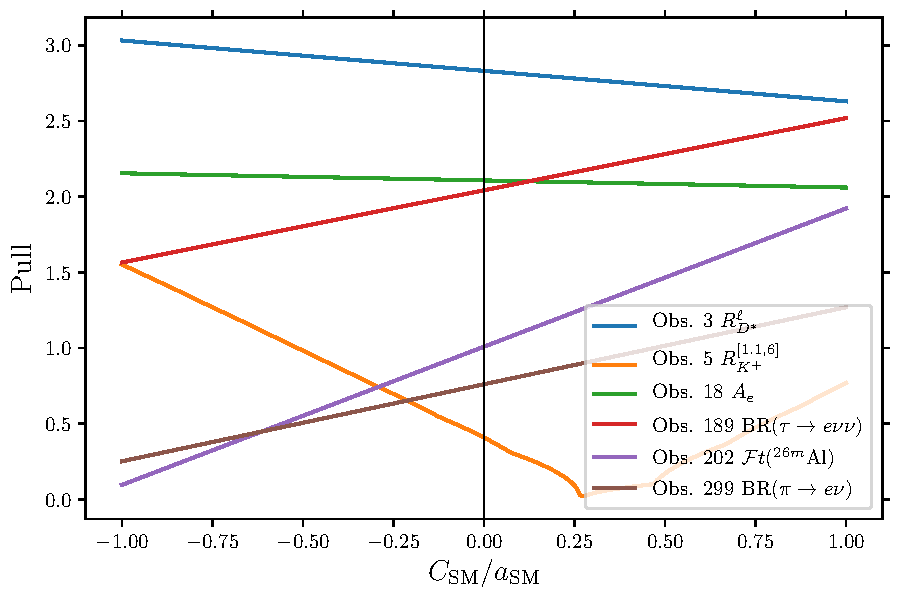
\includegraphics[width=\textwidth]{figures/evo_sm.pdf}
\end{column}
\begin{column}{0.40\textwidth}
    \begin{itemize}
        \item $R_{K^{(*)}}$, $R_{D^{(*)}}$ and EW observables show preference for larger deviations from SM.
        \item Nuclear $\beta$ decays and leptonic decays show preference for SM-like values.
    \end{itemize}
\end{column}
\end{columns}

\end{frame}

% \begin{frame}\frametitle{SMEFT Fit: Electron colliders}

% Electron colliders are powerful tools in testing neutral currents:
%     \begin{itemize}
%         \item Clean signatures.
%         \item Small uncertainties.
%         \item Detailed differential analyses in di-fermion final states.
%         \item Different longitudinal polarisation of the beams.
%         \item Experimental sensitivity increases with $\sqrt{s}$.
%     \end{itemize}

%     \begin{center}
%         \begin{columns}
%             \begin{column}{0.7\textwidth}
%                 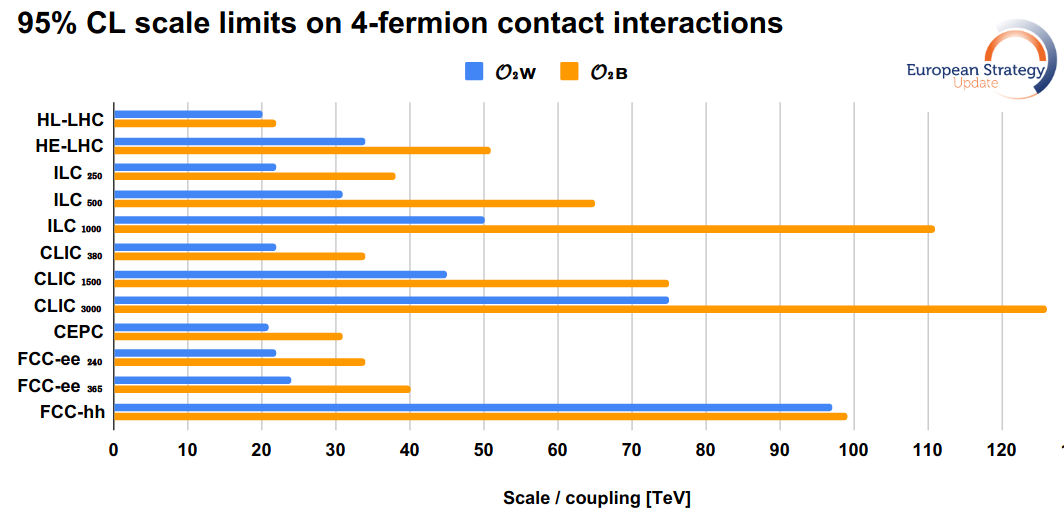
\includegraphics[width=\textwidth]{figures/operators_esu}
%             \end{column}
%             \begin{column}{0.19\textwidth}
%                 {\small$\begin{matrix}
%                             {\color[HTML]{4285f4} \mathcal{O}_{2W}} \Leftrightarrow \mathcal{O}_{\ell q(3)} \\ {\color[HTML]{ff9900} \mathcal{O}_{2B}} \Leftrightarrow \mathcal{O}_{\ell q(1)}
%                         \end{matrix}  $}
%             \end{column}
%         \end{columns}
% \colorcite{R. K. Ellis \textit{et al.} arXiv:1910.11775 [hep-ex]}
%     \end{center}

% \end{frame}

\begin{frame}\frametitle{SMEFT Fit: Improved EW prospects}
Electron colliders are powerful tools in testing neutral currents:
Clean signatures, small uncertainties,...\\[0.1em]
Effect of the improved precision in EW observables at ILC:
    \begin{center}
{\footnotesize Fit to $C_{\ell q}^e$ and $C_{\ell q}^\mu$ $\qquad\qquad\qquad   \qquad$ Fit to $C_{\ell q}^e = -C_{\ell q}^\mu$ and $C_{\ell q}^\tau$}
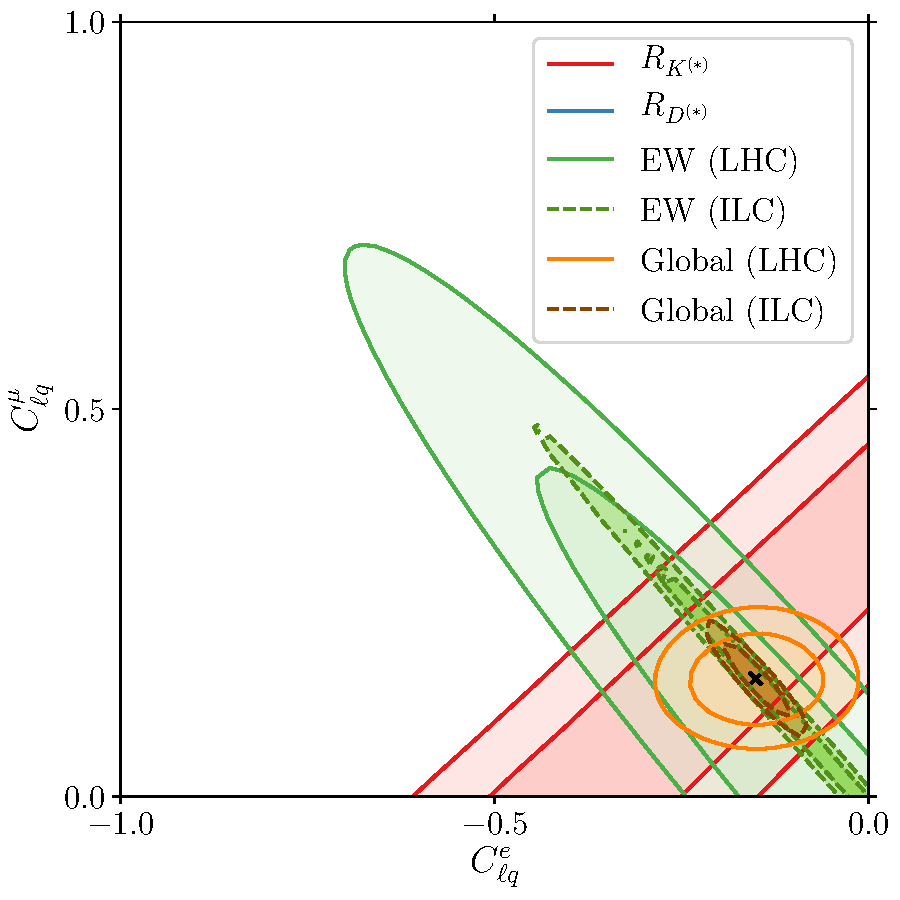
\includegraphics[width=0.40\textwidth]{figures/scIV_ILC.pdf}
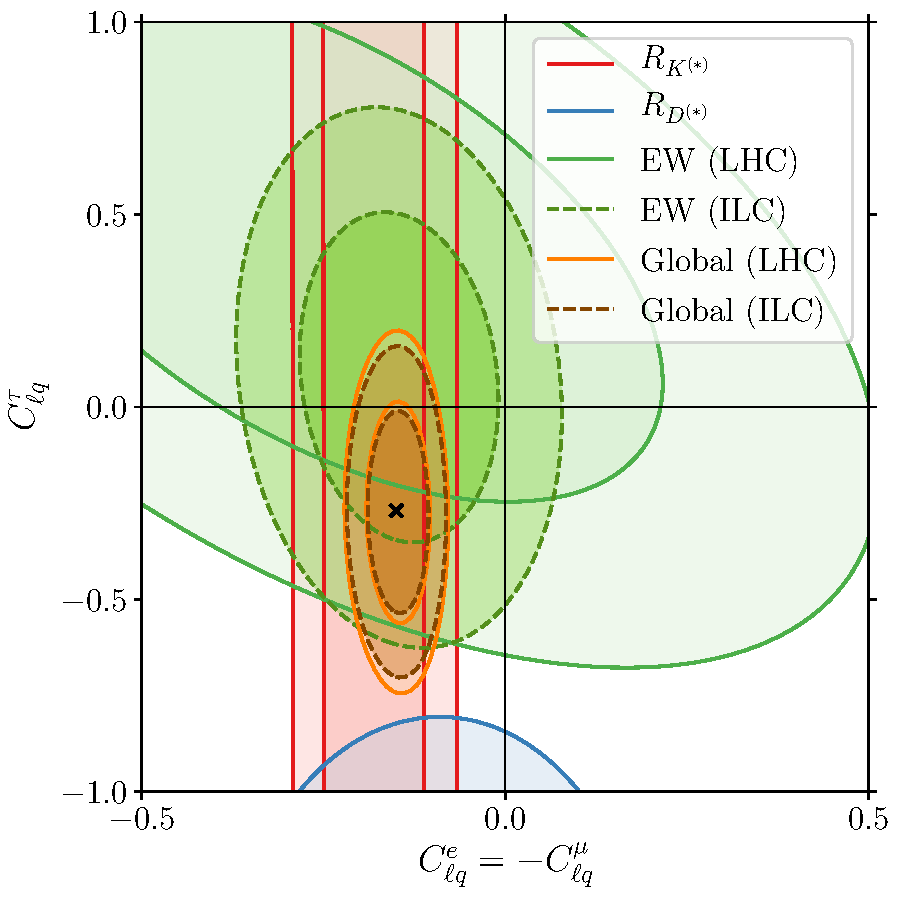
\includegraphics[width=0.40\textwidth]{figures/scXI_ILC.pdf}
    \end{center}

\begin{itemize}
    \item Lepton Flavour Universal New Physics ($C_{\ell q}^\mu+C_{\ell q}^e$) becomes very constrained.
    \item Lepton Flavour Universality violations ($C_{\ell q}^\mu-C_{\ell q}^e$) and $\tau$ physics mostly unaffected by the improved EW.
\end{itemize}

\end{frame}

\begin{frame}\frametitle{SMEFT Fit: Conclusions}

    \begin{itemize}
        \item Simplified phenomenological analysis of $B$-anomalies using SMEFT operators
              \begin{itemize}
                  \item $C_{\ell q}^\mu-C_{\ell q}^e$ contributes to  $R_{K^{(*)}}$.
                  \item $C_{\ell q}^\tau$ contributes to  $R_{D^{(*)}}$.
              \end{itemize}
\item We can explore the vicinity of the best fit point using the Hessian approximation.
\item Linear $e^+ e^-$ colliders will clear the picture by constraining the global fits through Electroweak precision tests.
    \end{itemize}

\end{frame}

\begin{frame}[plain] %%%ML Fit
\begin{block}{\huge Using Machine Learning techniques \\ in flavour physics}
    Chapter 7\\
    {\color{red} \textbf{J. Alda}, J. Guasch, S. Peñaranda,\\
    \textit{\footnotesize Using Machine Learning techniques in phenomenological studies in flavour physics,}\\
    arXiv:2109.07405 [hep-ph]}
\end{block}
\vspace{0.5cm}

\begin{columns}
\begin{column}{0.48\textwidth}
\begin{itemize}
\item Effective Field Theory
\item Global fits
\item Observables
\item Fit results
\item Exploring the likelihood function
\item \texttt{xgboost}
\item Machine Learning training
\item Machine Learning Montecarlo
\end{itemize}
\end{column}
\begin{column}{0.48\textwidth}
\begin{itemize}
\item SHAP values
\item SHAP values results
\item SHAP values and likelihood
\item Correlations between observables
\item $R_D$ and $\mathrm{BR}(B\to K^{(*)}\nu\bar{\nu})$
\item Connection to leptoquarks
\item Conclusions
\end{itemize}
\end{column}
\end{columns}

\end{frame}

\begin{frame}\frametitle{ML Fit: Effective Field Theory}
    \begin{itemize}
        \item NP only affects third generation leptons in the ``interaction basis''
              $$\mathcal{L}_\mathrm{SMEFT} = \frac{C_1}{\Lambda^2}(\bar{\ell}_3 \gamma_\mu \ell_3)(\bar{q}_3 \gamma^\mu  q_3) + \frac{C_3}{\Lambda^2}(\bar{\ell}_3 \gamma_\mu \tau^I \ell_3)(\bar{q}_3 \gamma^\mu \tau^I q_3).$$
\item Rotation from interaction basis. Flavour structure given by \colorcite{F.~Feruglio, P.~Paradisi and A.~Pattori. arXiv:1705.00929}

              $$C_{\ell q(1)}^{ijkl} = C_1 \lambda_\ell^{ij}\lambda_q^{kl}\,\qquad\qquad C_{\ell q(3)}^{ijkl} = C_3 \lambda_\ell^{ij}\lambda_q^{kl}\,. $$
              The mixing matrices must be hermitian, idempotent and with $\mathrm{tr}\lambda =1$. Parameterized as
              $$ \lambda = \frac{1}{1+|\alpha|^2+|\beta|^2}\begin{pmatrix}
                      |\alpha|^2 & \alpha \beta^* & \alpha \\ \alpha^* \beta & |\beta|^2 & \beta \\ \alpha^* & \beta^* & 1
                  \end{pmatrix}. $$
        \item The structure of the $\lambda$ matrices creates Lepton Flavour Violating effects through $\lambda_\ell^{ij}\, (i\neq j)$.
    \end{itemize}
\end{frame}

\begin{frame}\frametitle{ML Fit: Global fits}
    We perform global fits including $b\to s \ell^+\ell^-$ and
    $b\to c\ell\nu$ observables, and also electroweak precision tests,
    nuclear precision observables (superallowed $\beta$ decays) and Leptonic Flavour Violating observables.

    ~

    We consider two different scenarios:
    \begin{itemize}
\item \textbf{Scenario I:} Mixing to first generation $\alpha$ are negligible \\\colorcite{F.~Feruglio, P.~Paradisi and A.~Pattori. arXiv:1705.00929}.
\item \textbf{Scenario II:} Mixing to first and second generations \\{\scriptsize \color{red} \textbf{J. Alda}, J. Guasch and S. Peñaranda. arXiv:2109.07404}.
    \end{itemize}
    \begin{center}\small
        \begin{tabular}{|c|c|c|}\hline
                                        & Scenario I          & Scenario II                  \\\hline
            $C$                         & $-0.13 \pm 0.05$    & $-0.13 \pm 0.08$             \\\hline
            $\alpha^\ell$               &                     & $\pm (0.07^{+0.04}_{-0.07})$ \\\hline
            $\beta^\ell$                & $0 \pm 0.025$       & $0 \pm 0.025$                \\\hline
            $\alpha^q$                  &                     & $-0.05^{+0.12}_{-0.07}$      \\\hline
            $\beta^q$                   & $0.8^{+2.0}_{-0.5}$ & $0.73^{+2.8}_{-0.6}$         \\\hline
            $\Delta \chi^2_\mathrm{SM}$ & $40.32$             & $57.06$                      \\\hline
            SM Pull                     & $5.75\,\sigma$      & $6.57\,\sigma$               \\\hline
        \end{tabular}
    \end{center}

$\beta^\ell$ (mixing to the second generation of leptons) compatible with SM!
\end{frame}

\begin{frame}\frametitle{ML Fit: Observables}

    \begin{center}
        \begin{tabular}{lc}
            $R_{K^{(*)}} = \frac{\mathrm{BR}(B\to K^{(*)}\mu^+ \mu^-)}{\mathrm{BR}(B\to K^{(*)}e^+ e^-)}$ & $R_{D^{(*)}} = \frac{\mathrm{BR}(B\to D^{(*)}\tau \nu)}{\mathrm{BR}(B\to D^{(*)}\ell \nu)}$ \\
            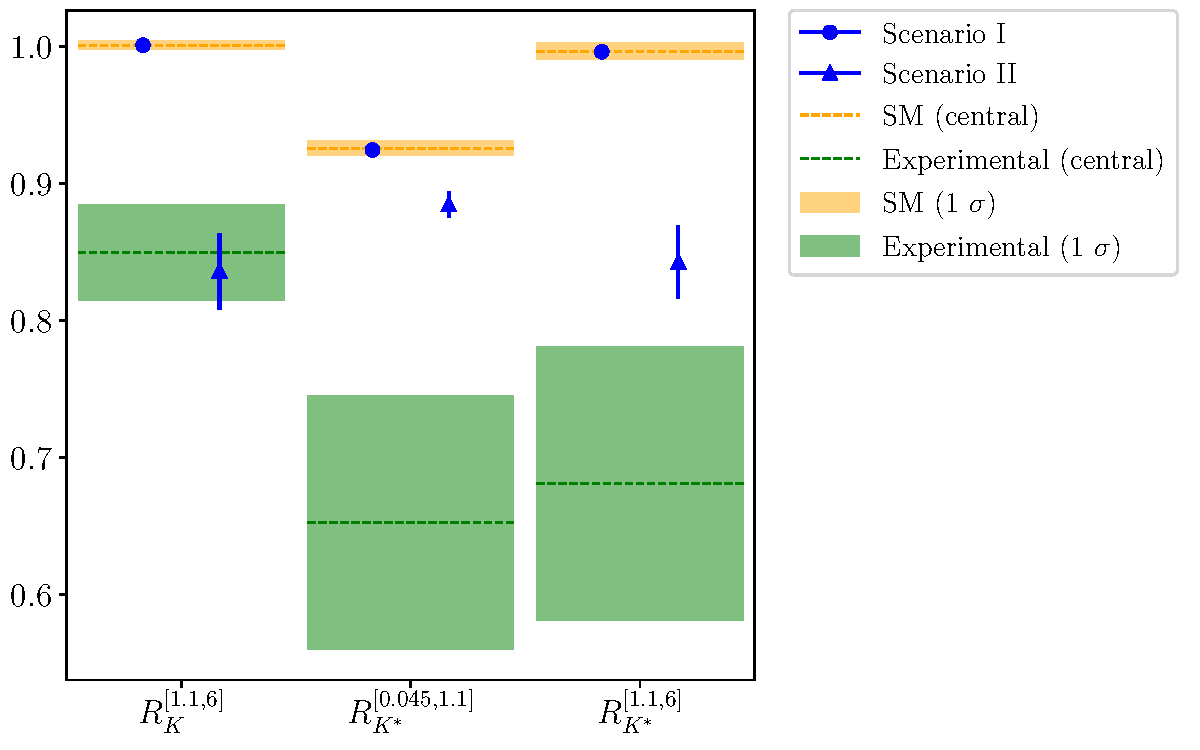
\includegraphics[width=0.55\textwidth]{figures/rotRKplot.pdf}                                 &
            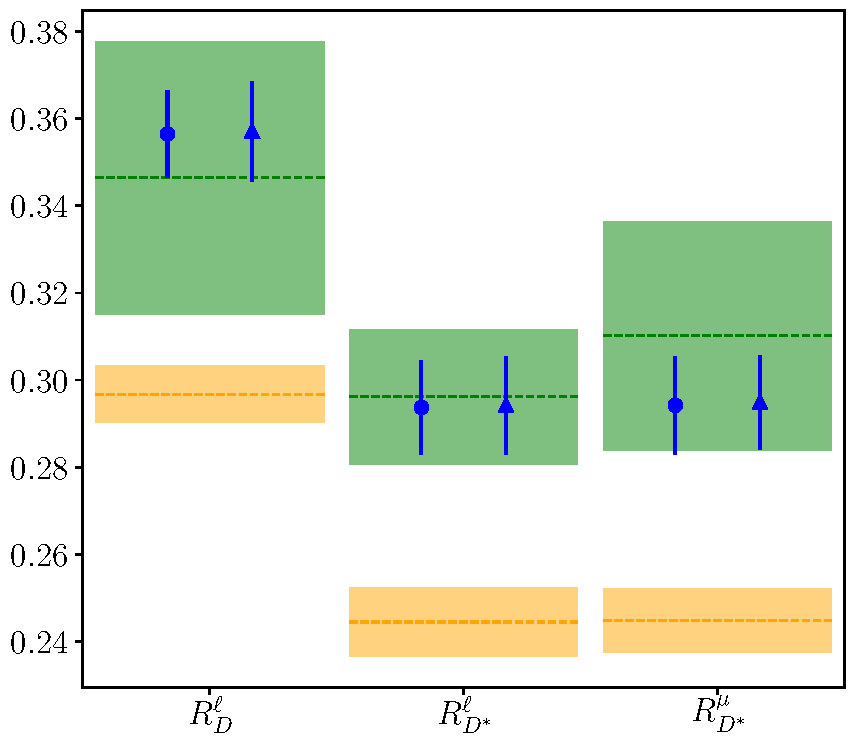
\includegraphics[width=0.4\textwidth]{figures/rotRDplot.pdf}
        \end{tabular}
    \end{center}
$R_{K^{(*)}}$ requires mixing with the first generation ($\alpha^\ell$).\\
The predictions for $R_{D^{(*)}}$ are in agreement with the experiments in both scenarios.


\end{frame}

\begin{frame}\frametitle{ML Fit: Fit results}
%Regions allowed at $1~\sigma$:
Two-dimensional sections of the
likelihood function $\Delta \log L$ in Scenario~II, at $1 \sigma$ and
$2 \sigma$:
    \begin{center}
        \begin{tabular}{cc}
{\small $\alpha^\ell$ and $\beta^\ell$}                         & {\small $\alpha^q$ and $\beta^q$}                               \\
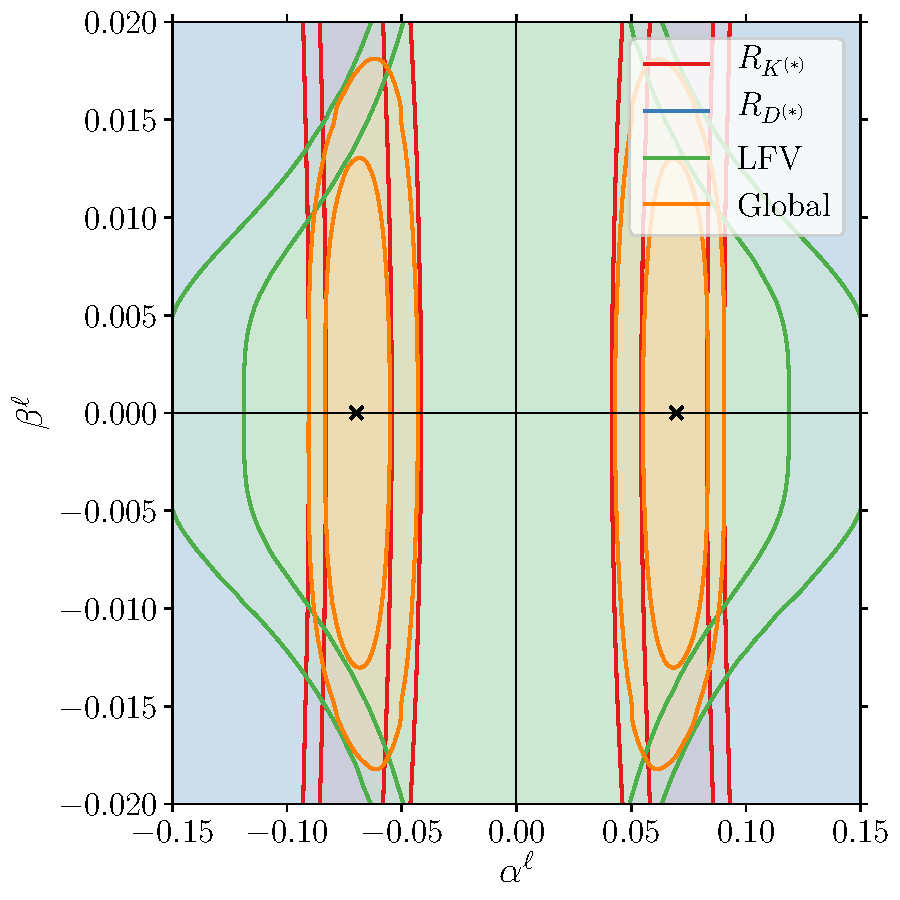
\includegraphics[width=0.34\textwidth]{figures/alphabeta_l.pdf} & 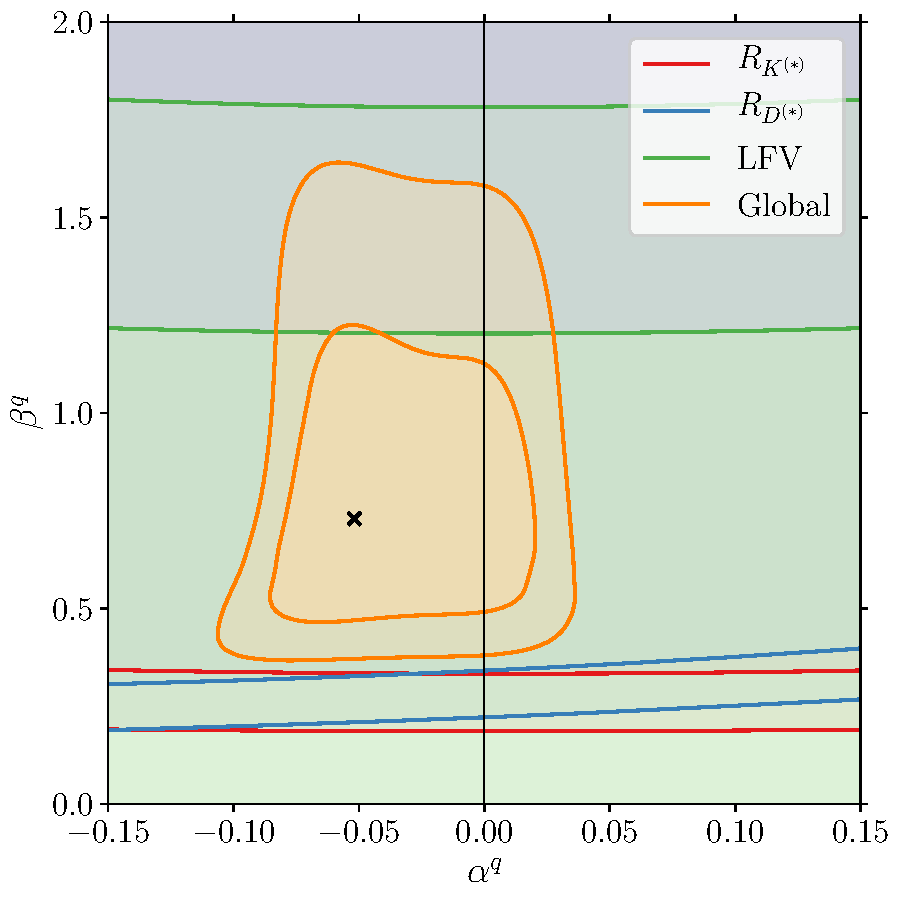
\includegraphics[width=0.34\textwidth]{figures/alphabeta_q.pdf}
        \end{tabular}
    \end{center}
    \begin{itemize}
        \item $\alpha^\ell$ is constrained by $R_{K^{(*)}}$.
        \item $\beta^\ell$ is constrained by LFV observables.
\item The regions of
equal probability are highly non-ellipsoidal\\
$\Rightarrow$ we cannot use
the Hessian approximation to characterise the fit.
\end{itemize}

\end{frame}

\begin{frame}\frametitle{ML Fit: Exploring the likelihood function}

    \begin{itemize}
        \item We would like to explore the properties of the likelihood function around the best fit point.
        \item {\bf Problem:} At each point $(C, \alpha^\ell, \beta^\ell, \alpha^q, \beta^q)$ requires the calculation of 471 observables, many of them need numerical integration.
        \item In the previous work, we used the Hessian approximation...

        \item ... but it doesn't work in this case because of non-linear relation between fit parameters and Wilson coefficients (equi-probability surfaces are not ellipsoids).
        \item {\bf Idea:} Teach a machine to approximate $\log L(\vec{C})$.
    \end{itemize}

\end{frame}

\begin{frame}\frametitle{ML Fit: xgboost}

    Regression tree
    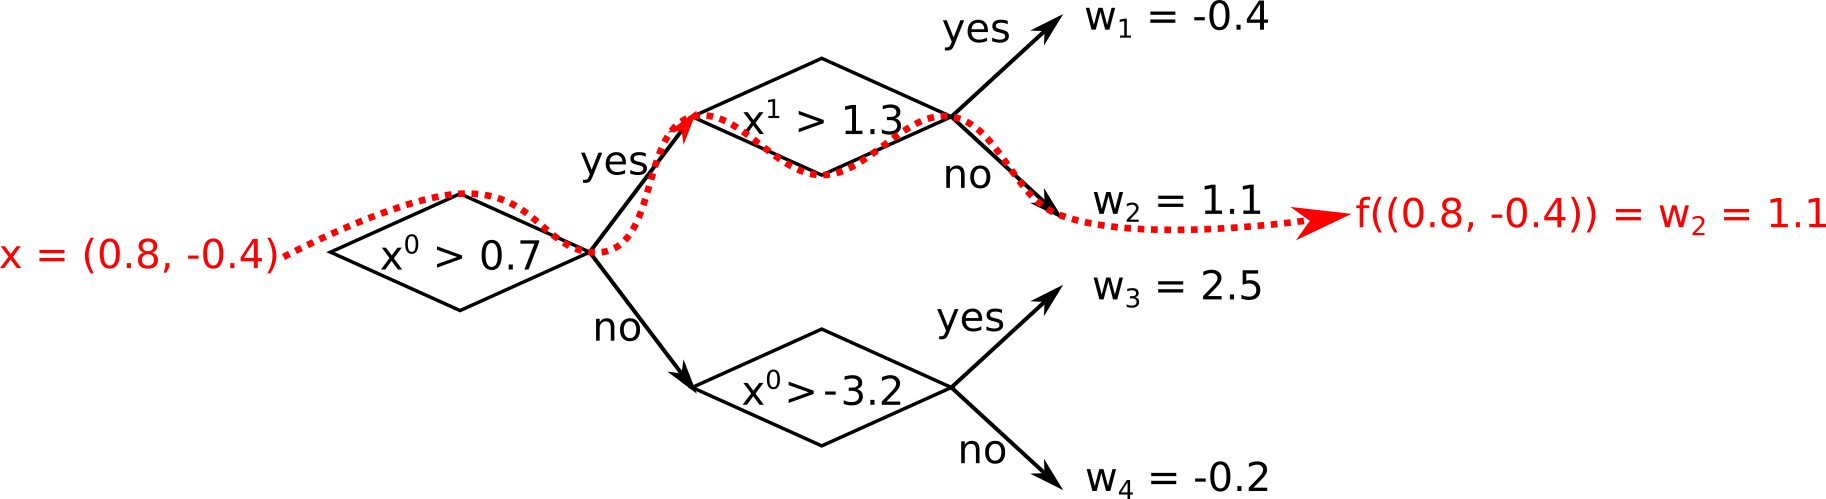
\includegraphics[width=\textwidth]{figures/regtree.png}

\vspace{1.0cm}

A regression tree $k$ defines a function $f_k(x)$. We use an
ensemble of trees $F$ for the prediction: $$\phi(x) = \sum_{k\in F}
    f_k(x)\,.$$\\
The function $\phi(x)$ will represent the approximation for the log-likelihood
function.
\end{frame}

\begin{frame}\frametitle{ML Fit: xgboost}

Extreme Gradient Boosting (xgboost) \\\colorcite{T.~Chen and C.~Guestrin. arXiv:1603.02754}.

    ~

    We have a dataset $\{(x_i, y_i)\}$ with $x_i \in X (\sim\mathbb{R}^n)$ and $y_i \in \mathbb{R}$, and want to find $\phi(x)$ so $\phi(x_i)\approx y_i$. Defining the regularized objective
$$\mathcal{L}[\phi] = \sum_i \ell(\phi(x_i), y_i) + \sum_k \Omega(f_k)\,.$$
    \begin{itemize}
        \item $\ell(\tilde{y}_i, y_i)$ is the loss function (Mean Absolute Error).
        \item $\Omega(f_k)$ penalizes the complexity of the trees.
    \end{itemize}
    The objective is optimized iteratively:
    \begin{itemize}
        \item The algorithm starts with one tree with a single leaf.
        \item At each step, one new tree with one more leaf is added to the ensemble (splitting).
        \item To prevent overfitting, the weights of the newly added leaf is multiplied by $\eta < 1$ (shrinkage).
    \end{itemize}
\end{frame}

\begin{frame}\frametitle{ML Fit: Machine Learning training}

    \begin{columns}
        \begin{column}{0.5\textwidth}
            Data sample consisting of
            \begin{itemize}
                \item 5000 points re-used from likelihood plots.
                \item 5000 random points.
                \item Split in 75\% training set, 25\% validation set.
            \end{itemize}
            Results of the training:
            \begin{itemize}
                \item Pearson regression coefficient $r=0.971$.
                \item Mean Absolute Error $0.655$.
            \end{itemize}
        \end{column}
        \begin{column}{0.5\textwidth}
Regression of the predicted values
of $\Delta\chi^2$ compared to the real ones in the validation
dataset:\\[0.2em]
            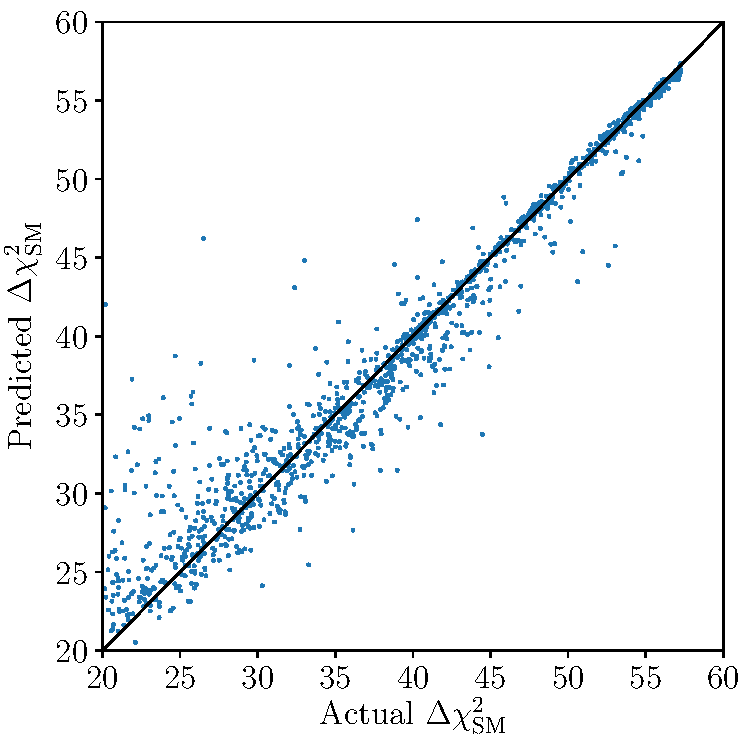
\includegraphics[width=\columnwidth]{figures/regression_xgb.pdf}
        \end{column}
\end{columns}

\end{frame}

\begin{frame}\frametitle{ML Fit: Machine Learning Montecarlo}
    \begin{columns}
        \begin{column}{0.5\textwidth}
            We want to generate a sample of points distributed according to the $\chi^2$ of the fit.

            We generate random points, that are accepted if
            $$\log \tilde{L}(\vec{C}) = \log L_\mathrm{bf} + \log u\,,$$
            with $u$ a random number from the uniform distribution in $[0,1)$. % chktex 9
        \end{column}
        \begin{column}{0.5\textwidth}
{\small Montecarlo points generated using the
Machine Learning algorithm:}\\[0.2em]
            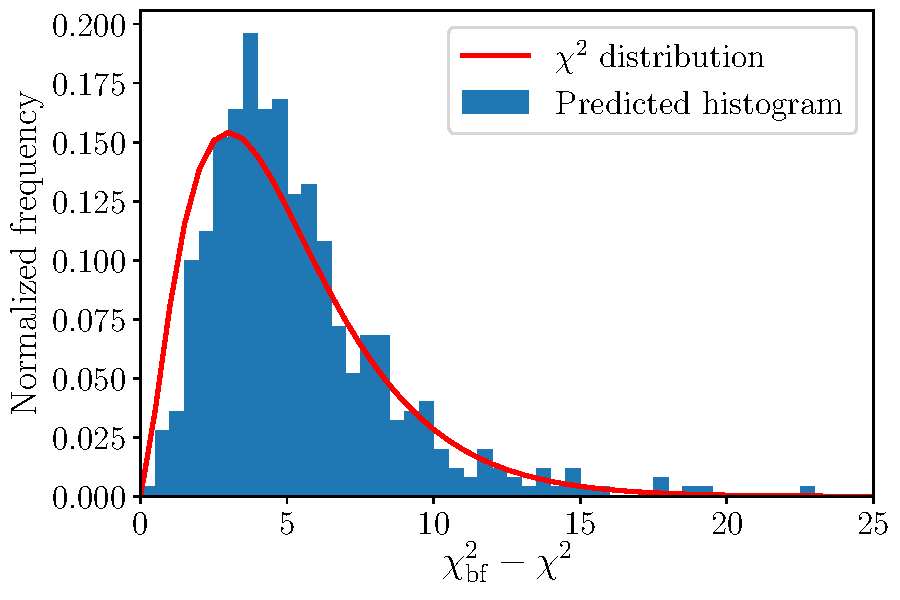
\includegraphics[width=\columnwidth]{figures/hist_xgb.pdf}
        \end{column}
    \end{columns}

    ~

We use the trained model $\log\tilde{L}(\vec{C})$ to compute an approximation of the likelihood function.

\end{frame}

\begin{frame}\frametitle{ML Fit: SHAP values}

Measure of the importance of each parameter in the Machine Learning
prediction for a single datapoint \colorcite{S. Lundberg,
    S. Lee. arXiv:1705.07874}.\\[0.3em]

We train $2^n$ simplified models\\[0.3em]

    \begin{columns}
        \begin{column}{0.5\textwidth}
            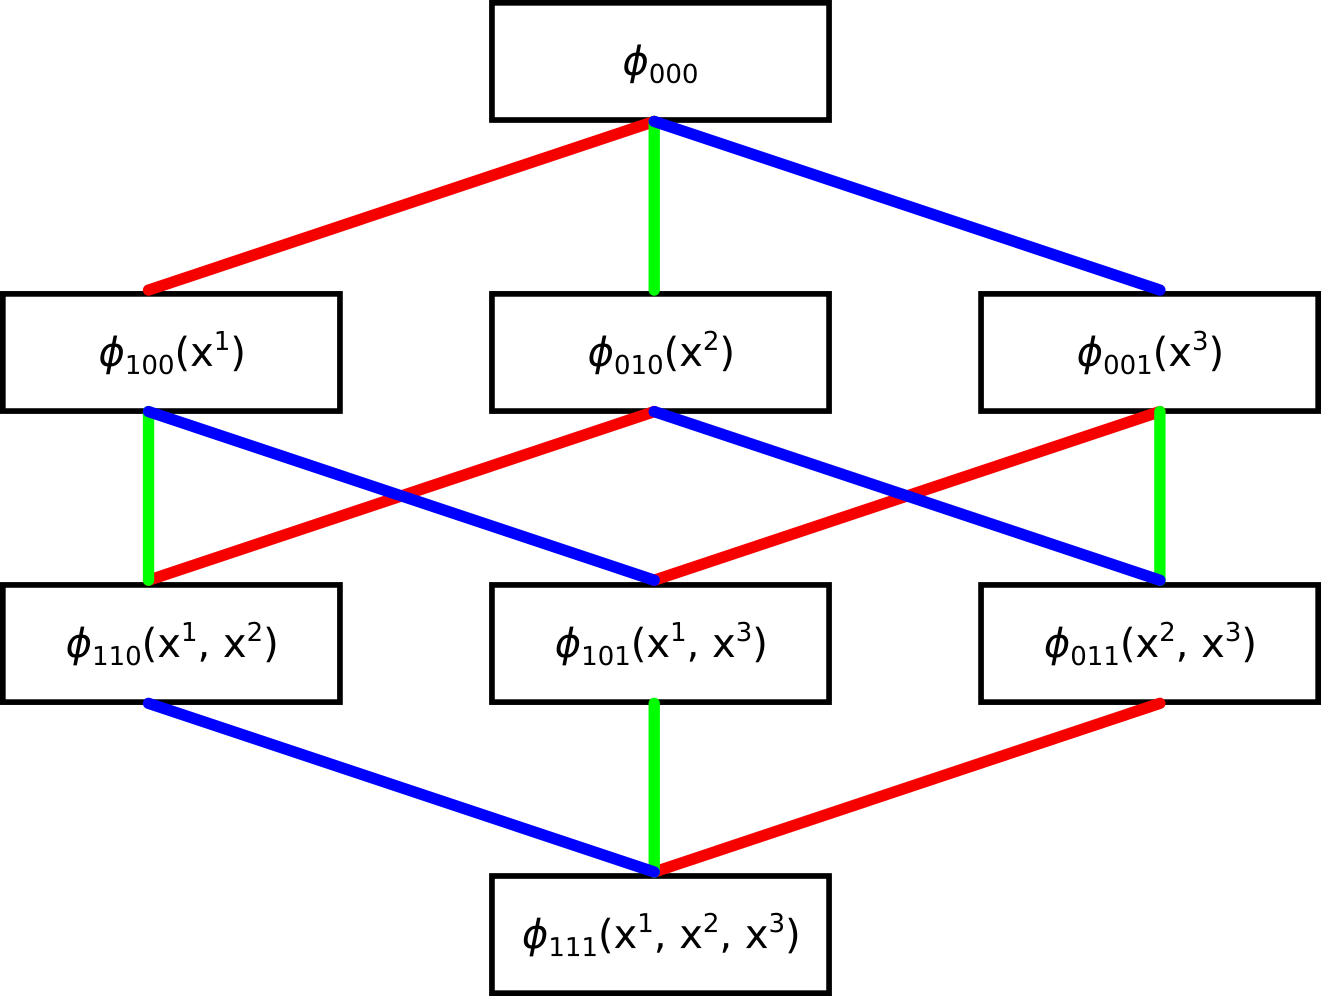
\includegraphics[width=\columnwidth]{figures/shapgraph.png}
        \end{column}
        \begin{column}{0.5\textwidth}
            \begin{itemize}
                \item Marginal contributions {\color{red} when adding $x^1$}: $\phi_{100}-\phi_{000}$, $\phi_{110}-\phi_{010}$, $\phi_{101}-\phi_{001}$, $\phi_{111} - \phi_{011}$.
                \item SHAP value {\color{red}for $x^1$} is a weighted average of all its marginal contributions.
\item $\phi_{000}$ is the constant value.\\[0.5em]
            \end{itemize}
        \end{column}
    \end{columns}

~

Efficient implementation (poly time) for tree-based Machine Learning models.\colorcite{S. Lundberg, G. Erion, S. Lee. arXiv:1802.03888}

\end{frame}

\begin{frame}\frametitle{ML Fit: SHAP values results}

    The mixing \(\beta^q\) to the second quark generation and $\alpha^\ell$ to the first lepton generation are in general the most important features.
    \begin{center}
        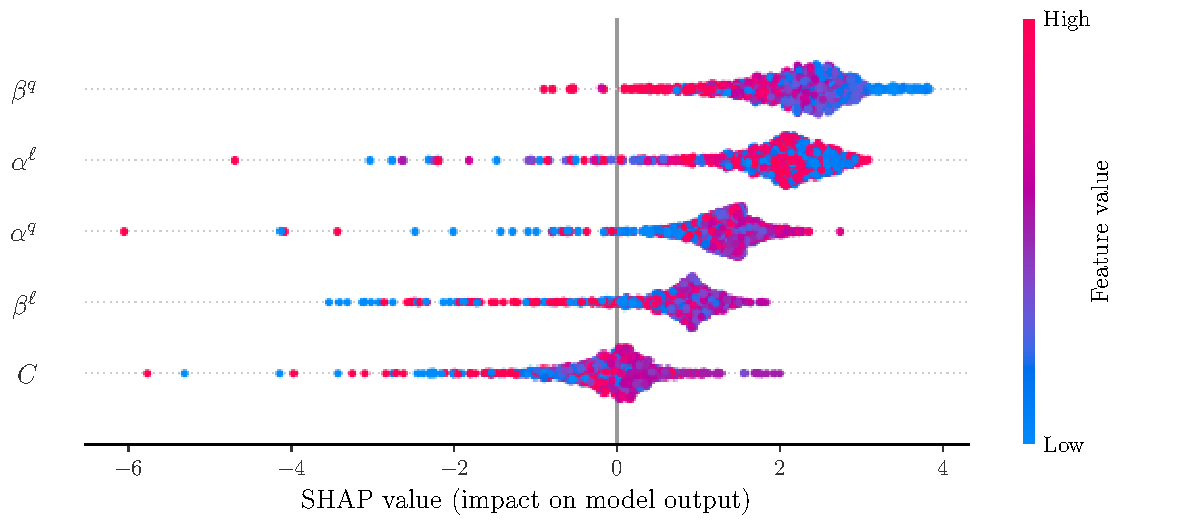
\includegraphics[width=0.8\textwidth]{figures/SHAP_summary.pdf}
    \end{center}

    For the best fit point, the value of $C$ is also important:
    \begin{center}
        \begin{tabular}{|*{8}{c|}}\hline
            Base  & \multicolumn{5}{c|}{SHAP value for} & Final         & Actual                                                        \\ \cline{2-6}
            value & $C$                                 & $\alpha^\ell$ & $\beta^\ell$ & $\alpha^q$ & $\beta^q$ & prediction & $\log L$ \\\hline
            39.43 & 3.293                               & 4.056         & 1.993        & 2.671      & 4.086     & 55.537     & 57.06    \\\hline
        \end{tabular}
\end{center}

\end{frame}

\begin{frame}\frametitle{ML Fits: SHAP values and likelihood}
    SHAP importances reproduce the dependence of the $-\log L$:
    \begin{center}
{\small \qquad\qquad$C\qquad\qquad\qquad\qquad \alpha^\ell \qquad\qquad\qquad\qquad\qquad\beta^q\qquad$} \\
\rotatebox{90}{\small $\qquad\Delta \log L$}
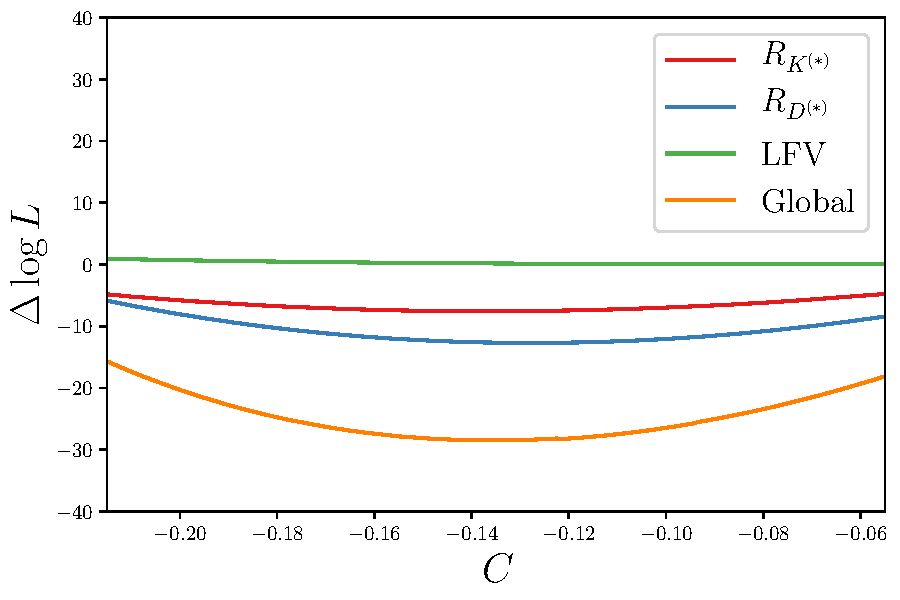
\includegraphics[width=0.30\textwidth]{figures/evoplot_C.pdf}
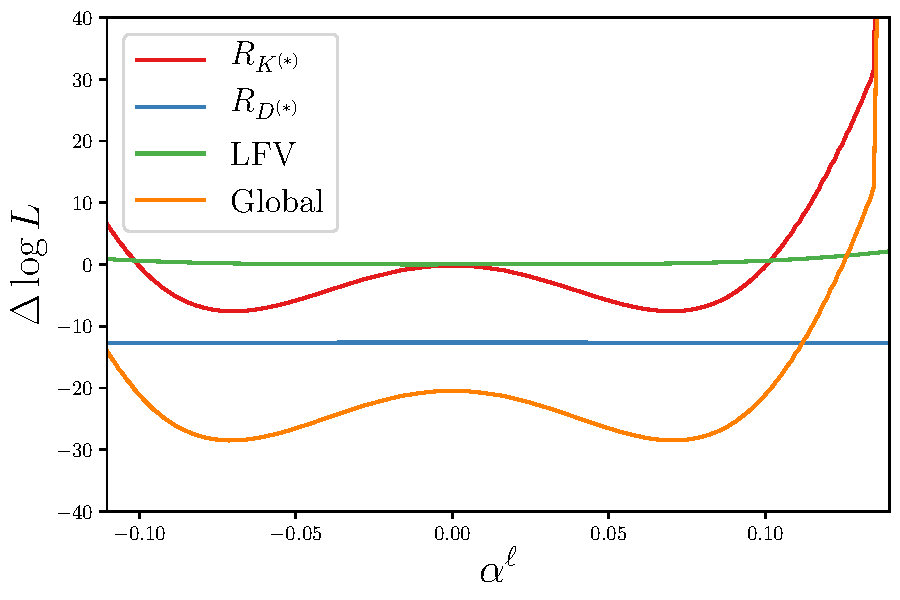
\includegraphics[width=0.30\textwidth]{figures/evoplot_alphal.pdf}
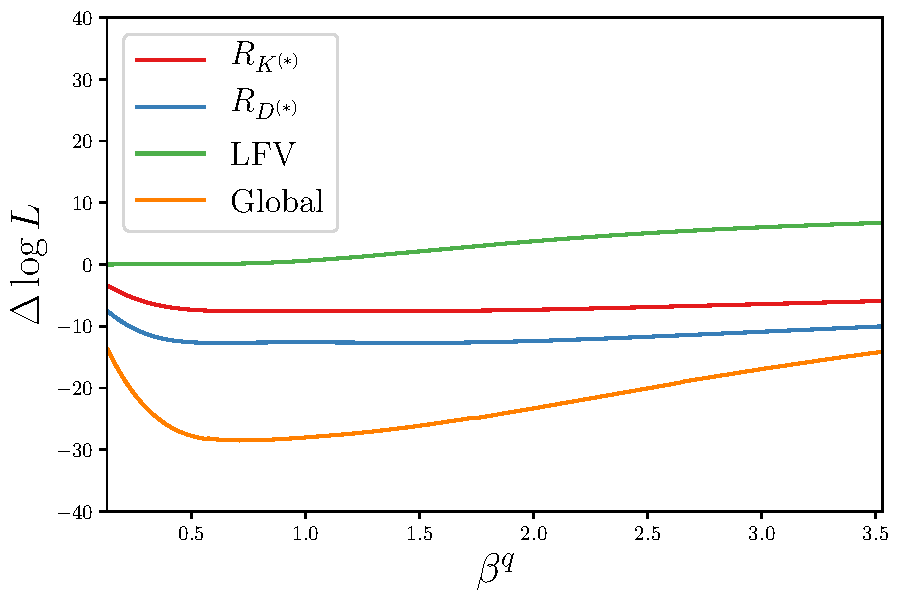
\includegraphics[width=0.30\textwidth]{figures/evoplot_betaq.pdf}
    \end{center}
    \begin{center}
\rotatebox{90}{\small $\qquad\qquad\mathrm{SHAP}$}
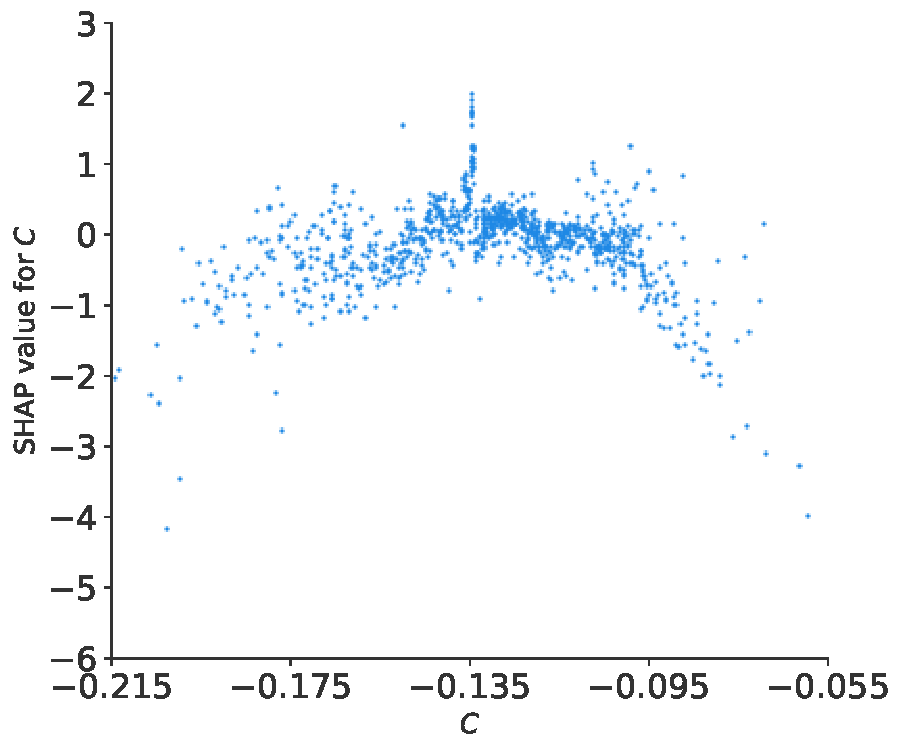
\includegraphics[width=0.30\textwidth]{figures/SHAP_C.pdf}
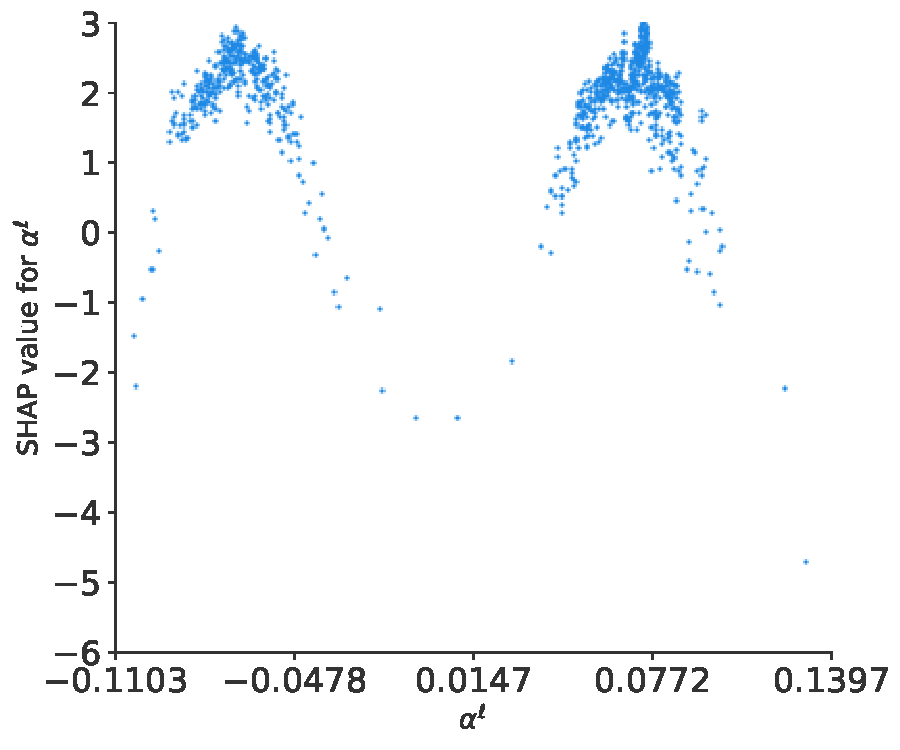
\includegraphics[width=0.30\textwidth]{figures/SHAP_al.pdf}
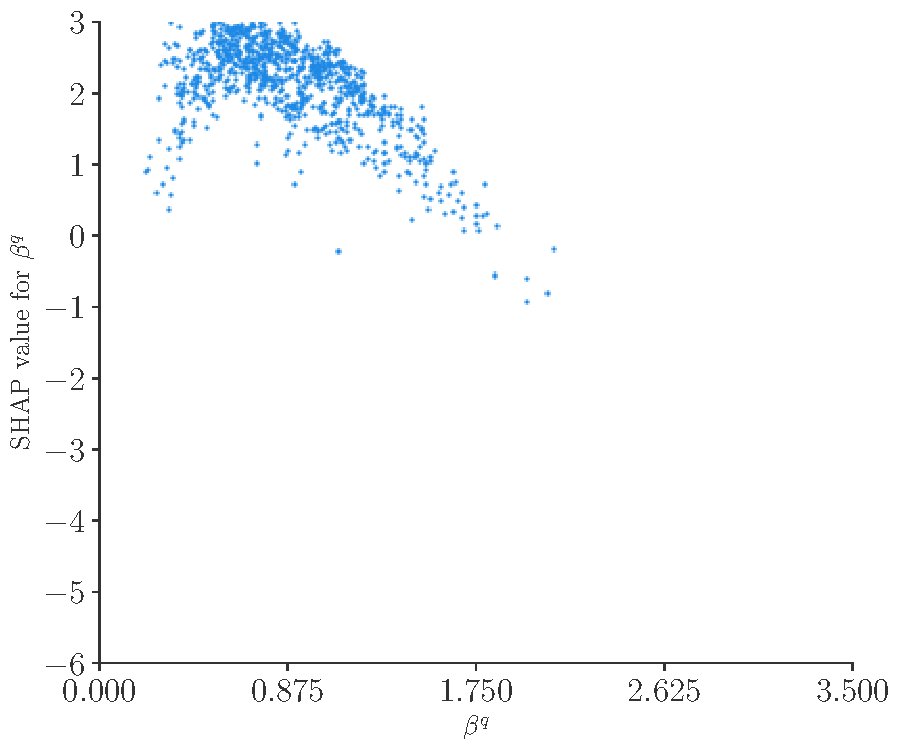
\includegraphics[width=0.30\textwidth]{figures/SHAP_bq.pdf}
    \end{center}
\begin{itemize}
    %\item Agreement between the results obtained by the
    %      Machine Learning Montecarlo algorithm proposed and the ones
    %      obtained by following the RG equations.
    \item The SHAP values reproduce correctly the
          general features of the fit.
\end{itemize}

\end{frame}

\begin{frame}\frametitle{ML Fits: Correlations between observables}
Matrix of Pearson correlation coefficients for selected observables in the 15000 points sample:
    \begin{columns}[onlytextwidth]
        \begin{column}{0.6\textwidth}
\begin{tikzpicture}
    \node[anchor=south west,inner sep=0] at (0,0) {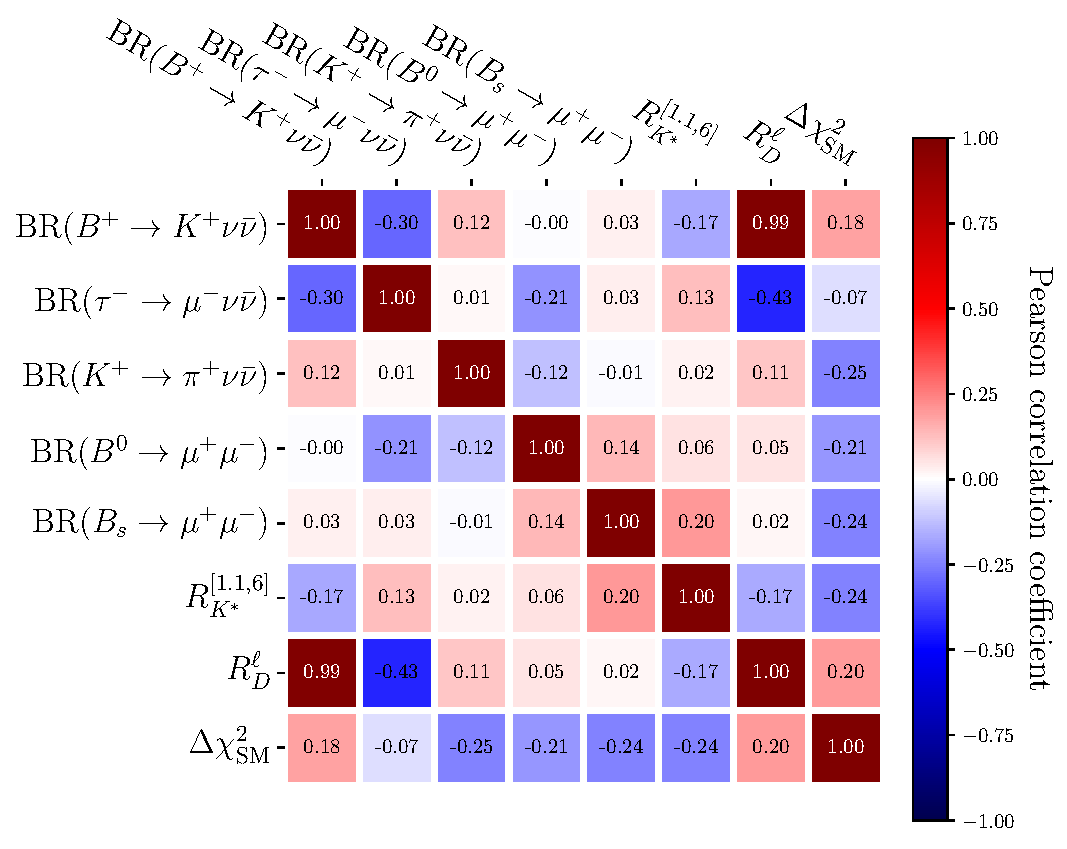
\includegraphics[width=\columnwidth]{figures/obscorr.pdf}};
    \draw[color = OliveGreen, line width=0.5mm] (1.95,1.1) circle (8pt);
    \draw[color = OliveGreen, line width=0.5mm] (4.7,3.8) circle (8pt);
\end{tikzpicture}

        \end{column}
        \begin{column}{0.4\textwidth}
            \begin{itemize}
                \item Moderate correlation between $R_K$ and $\mathrm{BR}(B_s \to \mu^+ \mu^-)$ because $C_9^\mu \neq C_{10}^\mu$.
                \item Also moderate correlation between $R_K$ and $R_D$.
\item {\color{OliveGreen}{Perfect correlation between} $R_D$
            $\mathrm{BR}(B\to K^{(*)}\nu\bar{\nu})$}.
                \item No observable displays large correlations to the global likelihood: global fits are needed.
            \end{itemize}
        \end{column}
\end{columns}

\end{frame}

\begin{frame}\frametitle{ML Fits: $R_D$ and $\mathrm{BR}(B\to K^{(*)}\nu\bar{\nu})$}

    \begin{center}
\begin{columns}[onlytextwidth]
    \begin{column}{0.55\textwidth}
        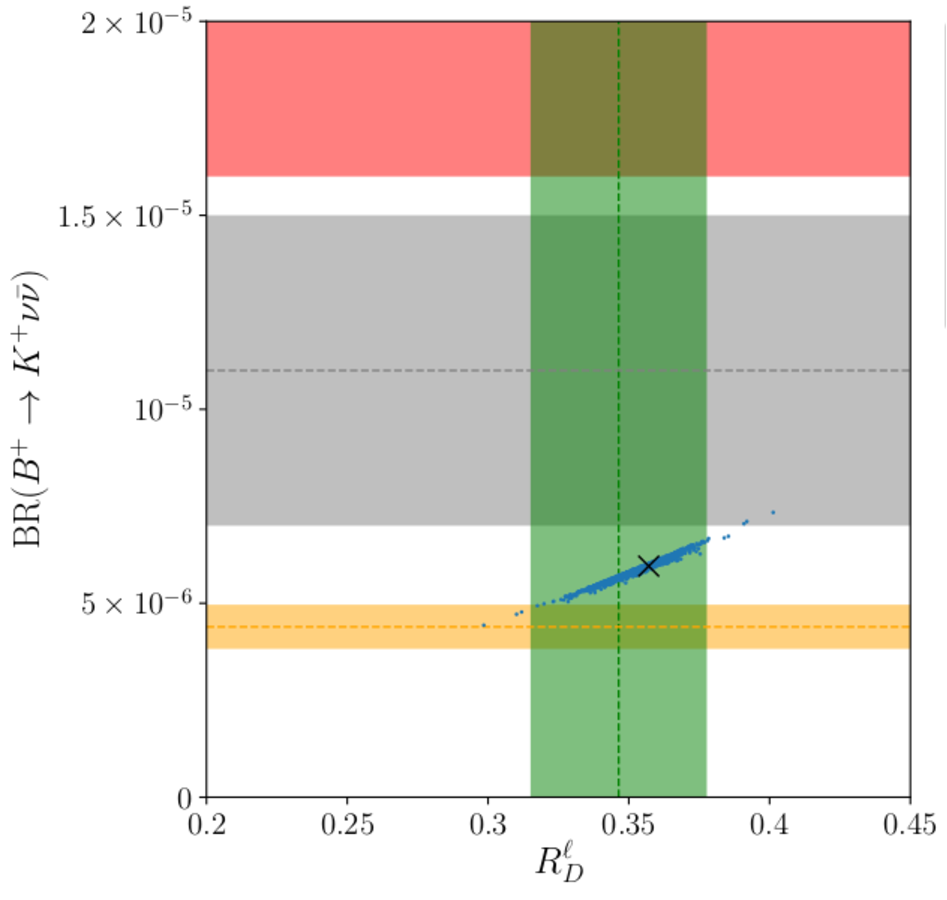
\includegraphics[width=\textwidth]{figures/RD_BKnunu_plot.pdf}
    \end{column}
    \begin{column}{0.45\textwidth}
        
\includegraphics[width=\textwidth]{figures/RD_BKnunu_leg1.pdf}\\[2pt]
        
\includegraphics[width=\textwidth]{figures/RD_BKnunu_leg2.pdf}\\[2pt]
        
\includegraphics[width=\textwidth]{figures/RD_BKnunu_leg3.pdf}\\[-6pt]
        \colorcite{Y. Ahmis \textit{et al.} (HFLAV) arXiv:1909.12524}\\[4pt]
        
\includegraphics[width=\textwidth]{figures/RD_BKnunu_leg4.pdf}\\[2pt]
        
\includegraphics[width=\textwidth]{figures/RD_BKnunu_leg5.pdf}\\[-6pt]
        \colorcite{J. Grygier \textit{et al.} (Belle) arXiv:1702.03224}\\[4pt]
        
\includegraphics[width=\textwidth]{figures/RD_BKnunu_leg6.pdf}\\[-6pt]
        \colorcite{F. Dattola (Belle-II) arXiv:2105.05754}
    \end{column}
\end{columns}

    \end{center}

    An excess in $R_D$ implies an excess in $\mathrm{BR}(B\to K^{(*)}\nu\bar{\nu})$. \\(Note that the {\color{gray}2021 World Average} is not included in our fit).

\end{frame}

\begin{frame}\frametitle{ML Fits: Connection to Leptoquarks}

    Vector Leptoquark $U_1 \sim (\bar{\mathbf{3}}, \mathbf{1}, 2/3)$,
    $$\mathcal{L}_{U_1} = x_L^{ij} \bar{q}_i \gamma_\mu U_1^\mu \ell_j + x_R^{ij} \bar{d}_{Ri} \gamma_\mu U_1^\mu e_{Rj} + \mathrm{h.c.} $$

    Matching to the SMEFT Wilson coefficients
    $$C_{\ell q(1)}^{ijkl} = C_{\ell q(3)}^{ijkl} = \frac{-\Lambda^2}{2M_U^2}x_L^{li}x_L^{kj*}\,,$$
    $$C_{ed}^{ijkl} = -\frac{1}{2}C_{qde}^{ijkl} = \frac{-\Lambda^2}{2M_U^2}x_R^{li}x_R^{kj*}\,,$$
    In terms of the parameters of our fit,
    $$|x_L^{ji}|^2 = -\frac{2}{M_U^2}C\lambda^\ell_{ii}\lambda^q_{jj}\,,$$
    $$\mathrm{Arg}(x_L^{ji}) = \mathrm{Arg}(\lambda_{j3}^q)-\mathrm{Arg}(\lambda_{i3}^\ell) + \theta\,.$$ % chktex 21

\end{frame}

\begin{frame}\frametitle{ML Fits: Connection to leptoquarks}

    Couplings to vector leptoquark $U_1$ in Scenario II (mixing to first and second generation):
    $$x_L = \begin{pmatrix}
            -2.27\times10^{-3}   & -3.76\times 10^{-10} & -0.0325            \\
            {\color{blue}0.0319} & 5.29\times 10^{-9}   & {\color{red}0.458} \\
            {\color{blue}0.0437} & 7.25\times 10^{-9}   & {\color{red}0.627}
        \end{pmatrix}\,.
    $$
    \begin{itemize}
\item Couplings {\color{red}$x_L^{23}$} and {\color{red}$x_L^{33}$}, previously proposed to describe the $R_{D^{(*)}}$ anomaly \colorcite{A.~Bhaskar, D.~Das, T.~Mandal, S.~Mitra and C.~Neeraj. 2101.12069}. Compatible with experimental limits.
        \item Additionally, couplings {\color{blue}$x_L^{21}$} and {\color{blue}$x_L^{31}$} to describe the $R_{K^{(*)}}$ anomaly.
    \end{itemize}

    ~

    Other leptoquark models, and $W'$ and $Z'$ models, do not generate $C_{\ell q(1)} = C_{\ell q (3)}$.
\end{frame}

\begin{frame}\frametitle{ML Fits: Conclusions}

    \begin{itemize}
        \item Using EFTs (SMEFT) to describe the $R_{K^{(*)}}$ and $R_{D^{(*)}}$ anomalies: $R_{D^{(*)}}$ generated at tree level and $R_{K^{(*)}}$ from interplay between tree and loop level.
        \item Global fits are needed to take in account possible side-effects.
        \item \texttt{xgboost} Machine Learning model is able to approximate the likelihood function.
        \item SHAP values capture the importance of each parameter in the fit.
        \item Interesting correlation between $R_{D^{(*)}}$ and $\mathrm{BR}(B\to K^{(*)}\nu\bar{\nu})$.
        \item Explanation in terms of vector leptoquark $U_1$ coupling to second and third generations of quarks and third ($R_{D^{(*)}}$) and first ($R_{K^{(*)}}$) generation of leptons.
    \end{itemize}

\end{frame}

\begin{frame}[plain] %%%ALPs
\begin{block}{\huge Leptonic meson decays into invisible ALP}
    Chapter 8 \\
    {\color{red}\textbf{J. Alda}, A. W. M. Guerrera, S. Peñaranda, S. Rigolin, \\
    \textit{Leptonic Meson Decays into invisible ALP,}\\
    Nuclear Physics B 979 (2022), 115791. arXiv:2111.02536 [hep-ph]}
\end{block}

\vspace{0.6cm}

\begin{columns}
\begin{column}{0.48\textwidth}
\begin{itemize}
\item Introduction
\item Effective Field Theory
\item Leptonic Meson Decays in ALP
\item Hadronic ALP emission
\end{itemize}
\end{column}
\begin{column}{0.48\textwidth}
\begin{itemize}
\item Leptonic ALP emission
\item Bounds on ALP-fermion couplings
\item Conclusions
\end{itemize}
\end{column}
\end{columns}

\vspace{0.6cm}
Research stay at \textit{Università degli Studi di Padova} (Italy)\\
\begin{center}
    
\includegraphics[height = 1.2cm]{logos/Padova.png}
\end{center}

\end{frame}

\begin{frame}\frametitle{ALPs: Introduction}
    \begin{itemize}
        \item Pseudo-scalar particles are common features of BSM models with a global $U(1)_\mathrm{PQ}$ symmetry spontaneously broken at scale $f_a \gg v$.
        \item Axion-like particles (ALP): mass $m_a$ is determined by UV physics, breaking the axion constraint $m_a f_a \approx m_\pi f_\pi$.
        \item ALP parameter space explored in a wide energy range:
              \begin{itemize}
                  \item Constraints on very light ALPs from astrophysics and cosmology.
                  \item Constraints for MeV-GeV range from fixed target facilities and $B$-physics experiments.
              \end{itemize}
        \item The goal of our work is to study the meson leptonic decays $M\to \ell \nu_\ell a$.
              \begin{itemize}
                  \item ALP escaping detection (long-lived $\tau_a \gtrsim 100\,\mathrm{ps} $ or decaying into a dark sector).
                  \item Generic ALP mass $m_a$ ($m_a \approx 10\ \mathrm{MeV}\sim 1\ \mathrm{GeV}$).
                  \item Generic flavour-conserving couplings to fermions.
              \end{itemize}
    \end{itemize}
\end{frame}

\begin{frame}\frametitle{ALPs: Effective Field Theory}
    The most general dimension-5 effective Lagrangian describing ALP-fermion flavour-conserving interactions is
    $$ \delta \mathcal{L}^{a}_{\mathrm{eff}} =
        -\frac{\partial_\mu a}{ 2 f_a} \sum_{i} c_i \,\overline{\psi}_i \gamma^\mu \gamma_5 \,\psi_i\,. $$
    Using the equations of motion, we can write the Lagrangian in the ``Yukawa'' basis instead of the derivative basis
    $$\delta \mathcal{L}^{a}_{\mathrm{eff}} = i \frac{a}{f_a} \sum_{i}  c_i\, m_i \, \overline{\psi}_i \gamma_5 \,\psi_i + \mathcal{O}(1/f_a^2) \,.$$
\end{frame}

\begin{frame}\frametitle{ALPs: Leptonic Meson Decays in ALP}
    \begin{itemize}
        \item At tree level, ALPs can be emitted either from the quarks in the initial meson, or from the final lepton.
              \vspace{0.5cm}

              ~

              {\centering
              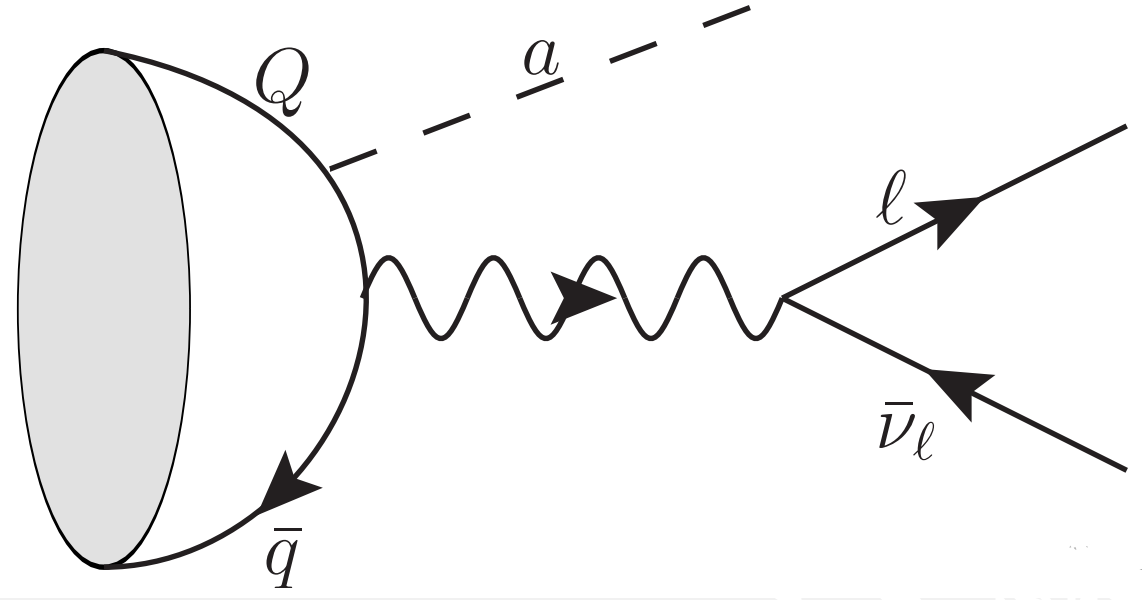
\includegraphics[width=0.4\textwidth]{figures/Lept1.1}$\qquad$
              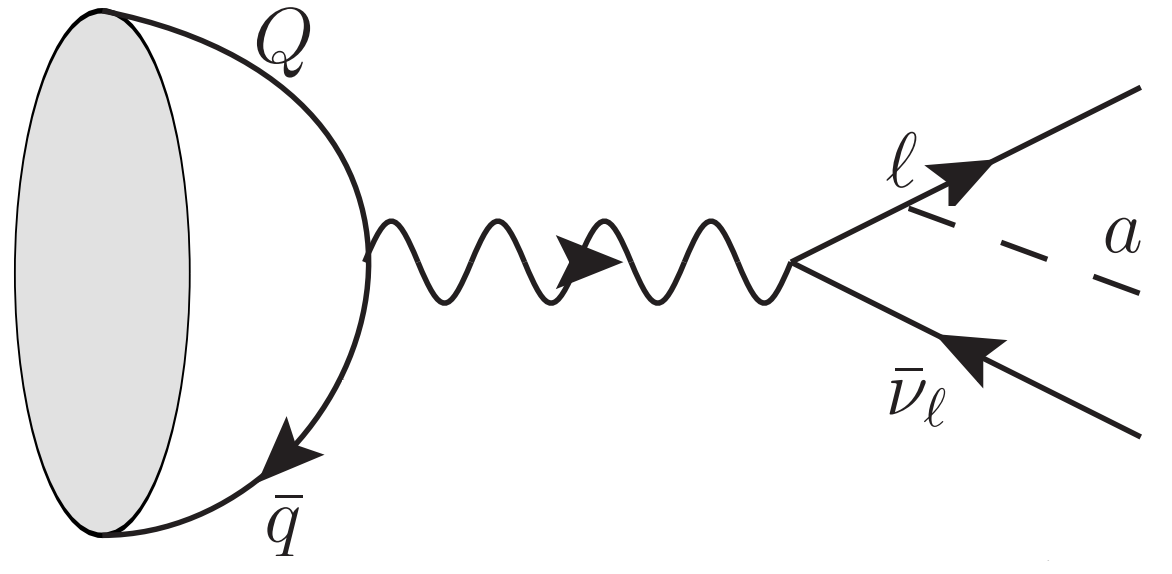
\includegraphics[width=0.4\textwidth]{figures/Lept1.3}}
              \vspace{0.5cm}
        \item The ALP coupling to neutrinos is negligible (proportional to $m_\nu$).
        \item The diagram for $W$ emission vanishes because the $W$-ALP coupling is proportional to the antisymmetric tensor.
    \end{itemize}
\end{frame}

\begin{frame}\frametitle{ALPs: Hadronic ALP Emission}
    The amplitude of ALP emission from quarks ($q$ is light $u$-type, and $Q$ is heavy $d$-type) is given by
    $$\mathcal{M}_h = \langle 0 |\bar{q}\,\Gamma^\mu_{h}\,Q|M\rangle \left(\bar{\ell} \,\gamma_\mu P_L \,\nu_\ell \right)\,,$$
    with $\Gamma^\mu_h$ given by
        {\small $$\Gamma^\mu_h = \frac{4 G_F}{\sqrt{2}} V_{qQ}
                \left(\frac{c_q\,m_q}{f_a}\,\gamma^\mu P_L\,\frac{\slashed{p}_a-\slashed{p}_q+m_q}{m_a^2 -2 p_a \cdot p_q}\,\gamma_5
                \,-\, \frac{c_Q\,m_Q}{f_a}\,\gamma_5\,\frac{\slashed{p}_a-\slashed{p}_q-m_Q}{m_a^2- 2 p_a \cdot p_Q}\,\gamma^\mu P_L \right)\,.$$}

    We need a hadronization model to calculate the hadronic matrix element $ \langle 0 |\bar{q}\,\Gamma^\mu_{h}\,Q|M\rangle$.

\end{frame}

\begin{frame}\frametitle{ALPs: Hadronization}
We follow the Lepage-Brodsky technique:\\
\colorcite{G. Lepage, S. J. Brodsky, Phys. Rev. D 22 (1980), p. 2157.}
    \begin{itemize}
        \item We parameterize the ground-state wavefunction of the meson as
              $$\Psi_M(x)=\frac{1}{4}\phi_M(x)\gamma^5(\slashed{P}_M + g_M(x) M_M)\,.$$
        \item The distribution of the fraction of momentum $x$ carried by the heavier quark is
              $$\phi_H(x) \propto  \left[\frac{\xi^2}{1-x}+\frac{1}{x}-1\right]^{-2} \qquad , \qquad \phi_L(x) \propto  x(1-x) \,,$$
              for heavy and light mesons respectively. $\xi\sim \mathcal{O}(m_q/m_Q)$.
        \item The hadronic elements are calculated integrating over the fractions of momentum,
              \begin{align*}
                  \langle 0| \bar{q}\,\Gamma^{\mu}\,Q |M\rangle          & = i f_M \int_0^1 dx\,\mathrm{Tr}\left[\Gamma^{\mu} \Psi_M (x)\right]\,, \\
                  \langle 0|\bar{q}\,\gamma^\mu \,\gamma_5 \,Q |M\rangle & = i f_M P_M^\mu \,.
              \end{align*}

    \end{itemize}
\end{frame}

\begin{frame}\frametitle{ALPs: Hadronic ALP Emission}
    One obtains the following decay amplitudes for the meson ALP--emission process:
    {\small $$\mathcal{M}_{h} = \frac{4\,i\,G_F\,V_{qQ}}{\sqrt{2}} \frac{f_M}{f_a} \frac{M_M^2}{2\,p_a \cdot P_M} \,
        \left[ c_Q \frac{m_Q}{M_M} \Phi^{(Q)}_M(m_a^2) - c_q \frac{m_q}{M_M} \Phi^{(q)}_M (m_a^2) \right]
        \left(\bar{\ell} \, \slashed{p}_a \,P_L \, \nu_\ell \right)$$}
    where the functions $\Phi^{(q,Q)}_M (m_a^2)$ contain the integrals over the quark momentum fraction.

    ~

Improvements compared to previous results \colorcite{Y. Aditya, K. J. Healey, A. A. Petrov. 1201.1007 [hep-ph]}:
    \begin{itemize}
        \item Formula for massive ALPs.
        \item We do not rely on the assumption $c_q = c_Q$.
\item Corrected a factor 1/2 in the published formula for massless decays.
    \end{itemize}

\end{frame}

\begin{frame}\frametitle{ALPs: Leptonic ALP Emission}
    The leptonic decay amplitude for the lepton ALP--emission process can be obtained straight-forward
    $$ \mathcal{M}_\ell =  \langle 0|\bar{q}\,\gamma_\mu  P_L\,Q |M\rangle \left(\bar{\ell} \,\Gamma^\mu_\ell \,\nu_\ell \right) \,,
    $$
    with
    $$
        \Gamma^\mu_\ell = - \frac{4 G_F}{\sqrt{2}} V_{qQ}
        \left(\frac{c_\ell\,m_\ell}{f_a}\,\gamma_5\,\frac{\slashed{p}_a+\slashed{p}_\ell+m_\ell}{m_a^2 + 2 p_a \cdot p_\ell}\,\gamma^\mu P_L \right)\,.$$

    The amplitude is
    $$\mathcal{M}_\ell = - \frac{4\,i\, G_F}{\sqrt{2}} V_{qQ} \,\frac{f_M}{f_a}  \left[  c_\ell\,m_\ell\, \left(\bar{\ell} \, P_L \,\nu_\ell \right) -
            \frac{ c_\ell \, m^2_\ell}{m_a^2\,+\, 2\,p_a\cdot p_\ell} \left(\bar{\ell} \, \slashed{p}_a\, P_L \,\nu_\ell \right) \right] \,.$$
\end{frame}

\begin{frame} \frametitle{ALPs: Bounds on ALP-fermion couplings}
    Bounds on leptonic meson decays coming from particle physics experiments:
    \begin{itemize}
        \item $B$ meson decays: $B$-factories (Belle).
        \item Charmed meson decays: BESS, Belle.
        \item Kaon decays: KLOE and NA62.
    \end{itemize}

    ~

    We set the bounds to $c_i$ by demanding that
    $$
        \begin{matrix}
            \mathrm{BR}(M\to \ell + \mathrm{inv}) \\
            (1\,\sigma)
        \end{matrix} = \left\{ \begin{matrix}
            \mathrm{BR}(M\to \ell \nu)   &   & [\mathrm{SM}]  \\
                                         & + &                \\
            \mathrm{BR}(M\to \ell \nu a) &   & [\mathrm{ALP}]
        \end{matrix} \right.
    $$

\end{frame}

\begin{frame}\frametitle{ALPs: Bounds on ALP-$u$ couplings}
    ALP couplings to $u$-quarks
    \begin{columns}
        \begin{column}{0.5\textwidth}
            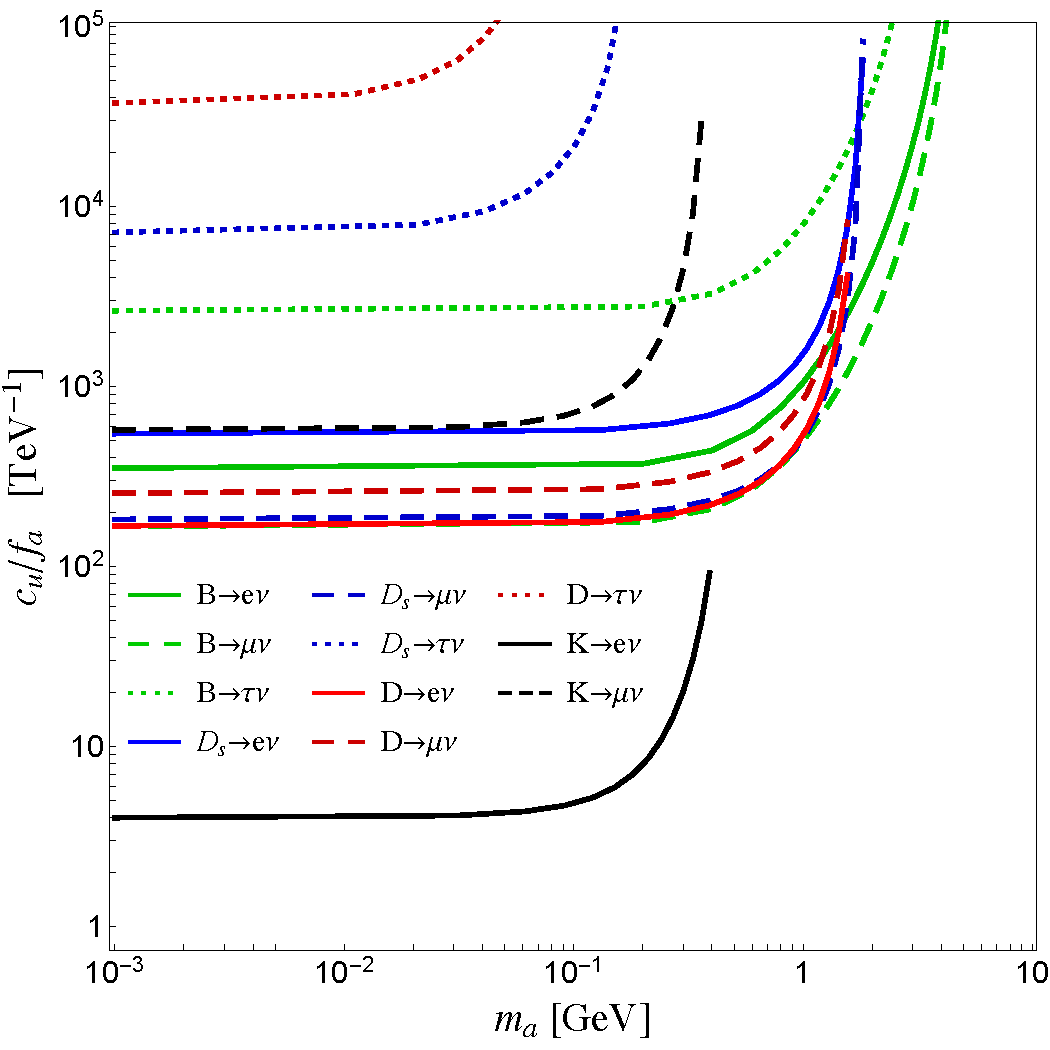
\includegraphics[width=\columnwidth]{figures/Fig2aS}
        \end{column}
        \begin{column}{0.5\textwidth}
            \begin{itemize}
                \item Bounds not competitive compared to top-enhanced penguin decays and tree-level FCNC processes.
                \item Only exception in $K\to e \nu_e$ decays.
                \item Limits to the scale $f_a \gtrsim 10^3- 10^4~\mathrm{MeV}$ for light lepton decays and $f_a \gtrsim 10^1 - 10^2~\mathrm{MeV}$ for $\tau$ decays.
            \end{itemize}
        \end{column}
    \end{columns}
\end{frame}

\begin{frame}\frametitle{ALPs: Bounds on ALP-$d$ couplings}
    ALP couplings to $d$-quarks
    \begin{columns}
        \begin{column}{0.5\textwidth}
            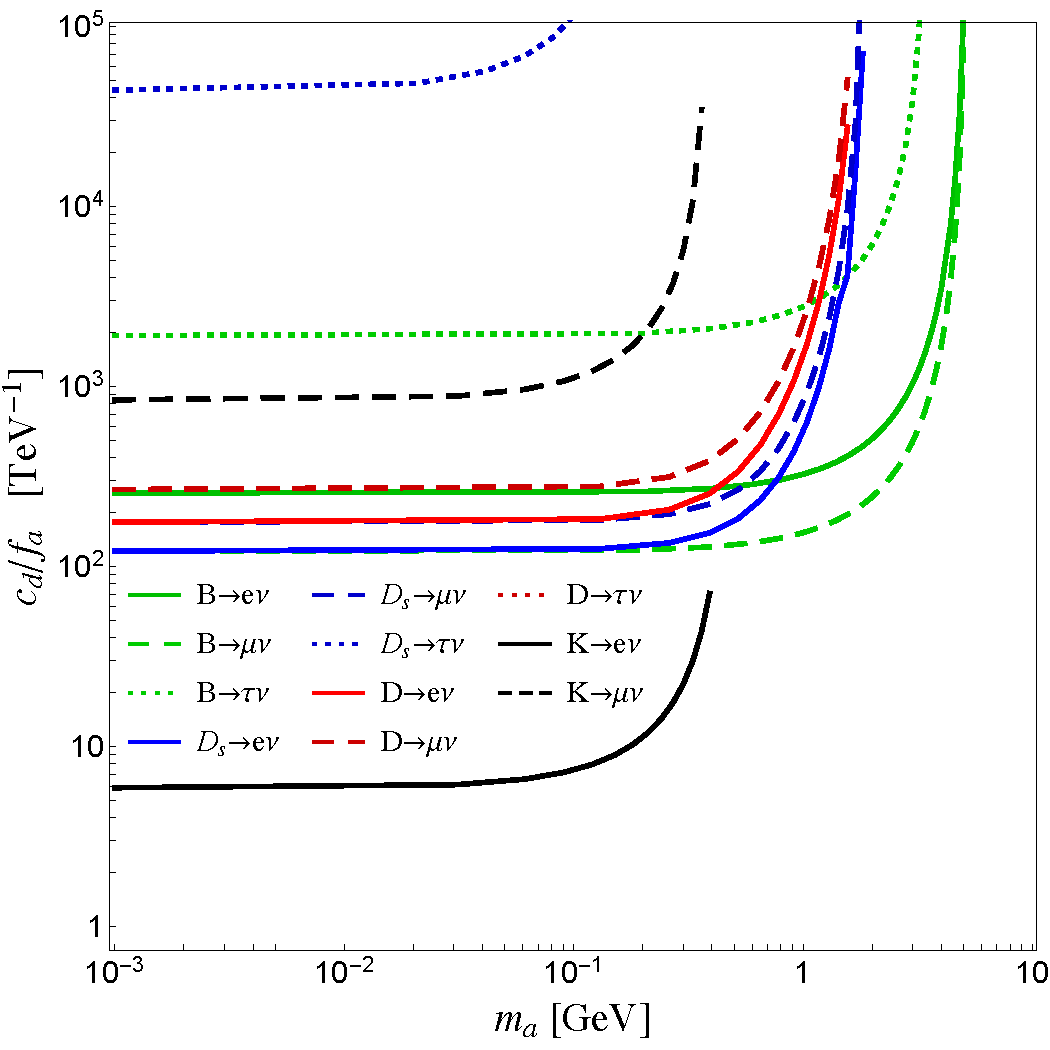
\includegraphics[width=\columnwidth]{figures/Fig2bS}
        \end{column}
        \begin{column}{0.5\textwidth}
            \begin{itemize}
                \item Bounds not competitive compared to $\Upsilon(ns)$ decays.
                \item Only exception in $K\to e \nu_e$ decays.
                \item Limits to the scale $f_a \gtrsim 10^3- 10^4~\mathrm{MeV}$ for light lepton decays and $f_a \gtrsim 10^1 - 10^2~\mathrm{MeV}$ for $\tau$ decays.
            \end{itemize}
        \end{column}
    \end{columns}
\end{frame}

\begin{frame}\frametitle{ALPs: Bounds on ALP-lepton couplings}
    ALP couplings to leptons
    \begin{columns}
        \begin{column}{0.5\textwidth}
            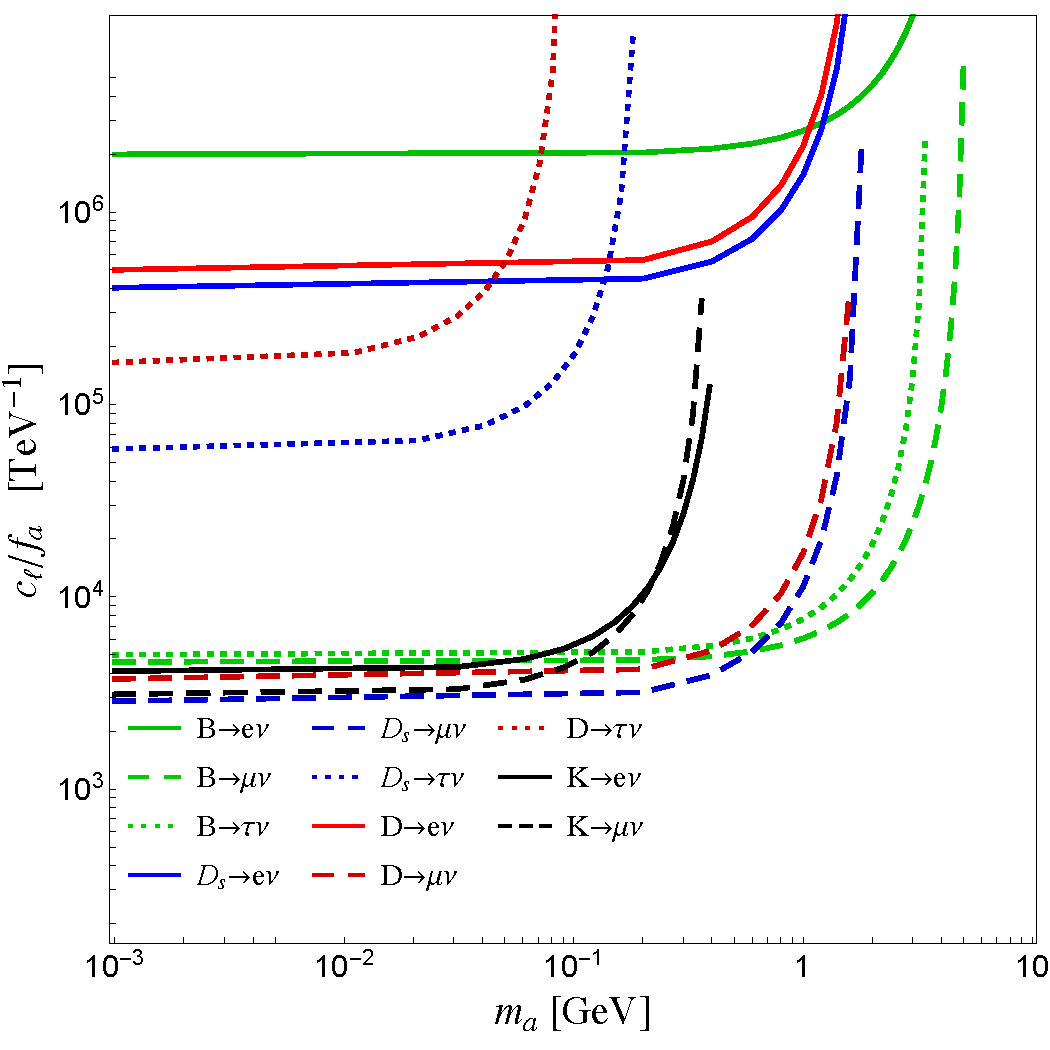
\includegraphics[width=\columnwidth]{figures/Fig3aS}
        \end{column}
        \begin{column}{0.5\textwidth}
            \begin{itemize}
                \item Best bounds available for invisible ALP.
                \item Better results for muons, $f_a \gtrsim 10^2 - 10^3~\mathrm{MeV}$.
                \item Electrons are mass-suppressed, $f_a \gtrsim 1~\mathrm{MeV}$.
                \item Results on ALP-electron couplings can be complementary to future DM searches (EDELWEISS, LDMX) and reactor searches (CONNIE, CONUS, MINE, $\nu$-cleus).
            \end{itemize}
        \end{column}
    \end{columns}
\end{frame}

\begin{frame}\frametitle{ALPs: Bounds on ALP-fermion couplings}
Our results show an improvement of $~$ one order of magnitude compared to the previous published bounds \colorcite{Y. Aditya, K. J. Healey, A. A. Petrov. 1201.1007 [hep-ph]}:
    \begin{itemize}
        \item Improvement of the experimental determination of pseudo-scalar leptonic decays.
        \item Correction of the 1/2 factor in the hadronic amplitude.
        \item Individual analysis of each fermion flavour. This removes a partial cancellation between $c_q$ and $c_Q$.
    \end{itemize}
\end{frame}

\begin{frame}
    \frametitle{ALPs: Bounds on ALP-fermion couplings}
    We also trialed calculating the bounds using the differential distribution.
    \begin{columns}
        \begin{column}{0.6\textwidth}
            \center
            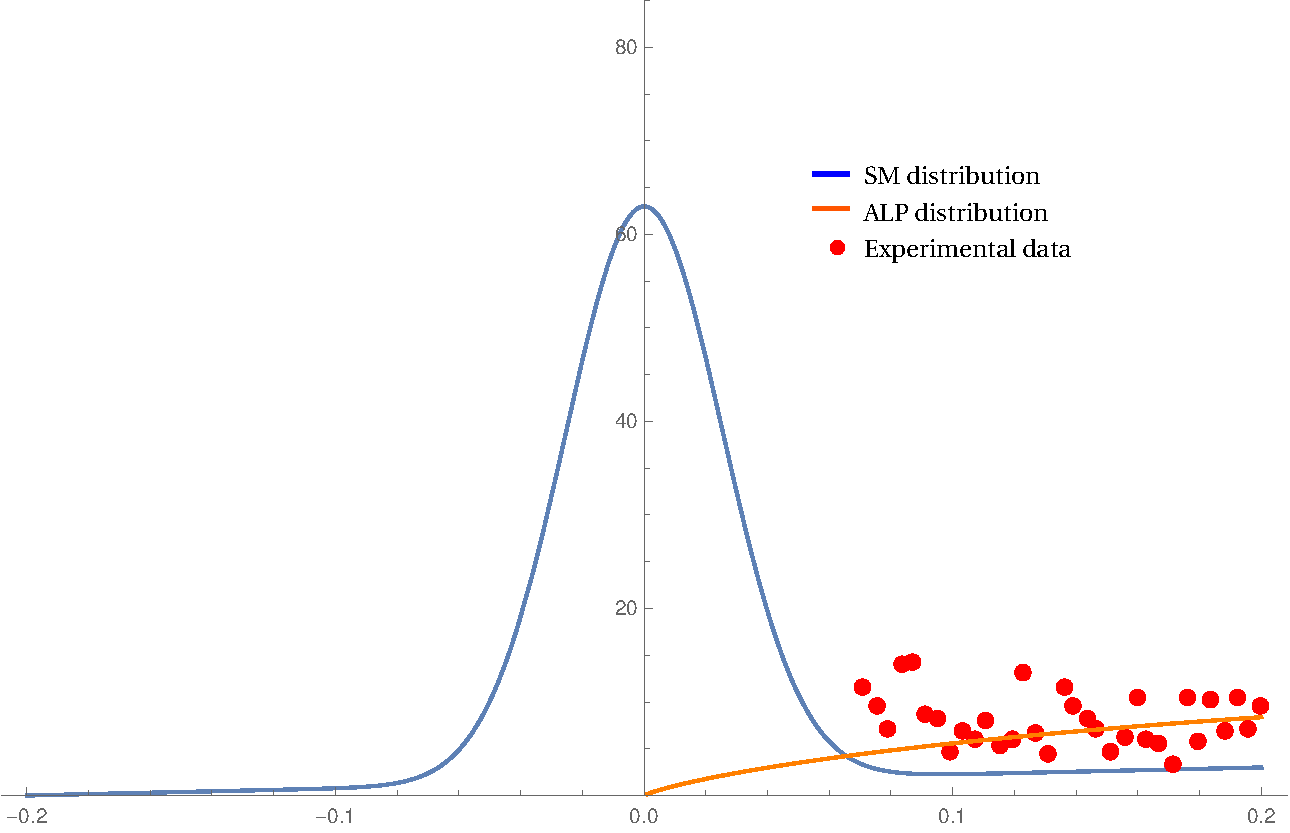
\includegraphics[width=\columnwidth]{figures/distr}
            {\small $M_\mathrm{miss}^2\ [\mathrm{GeV}^2]$}
        \end{column}
        \begin{column}{0.4\textwidth}
            In a three-body decay, the differential distribution $d\Gamma/d s$ ($s \equiv M_\mathrm{miss}^2$) is not centered around $M_\mathrm{miss}=0$.

            ~

            We can obtain bounds using only the experimental data in the tail of the differential distribution.
        \end{column}
    \end{columns}
\end{frame}

\begin{frame}\frametitle{ALPs: Bounds on ALP-fermion couplings}
    $D_s \to \mu \nu_\mu$ decay
    \begin{columns}
        \begin{column}{0.5\textwidth}
            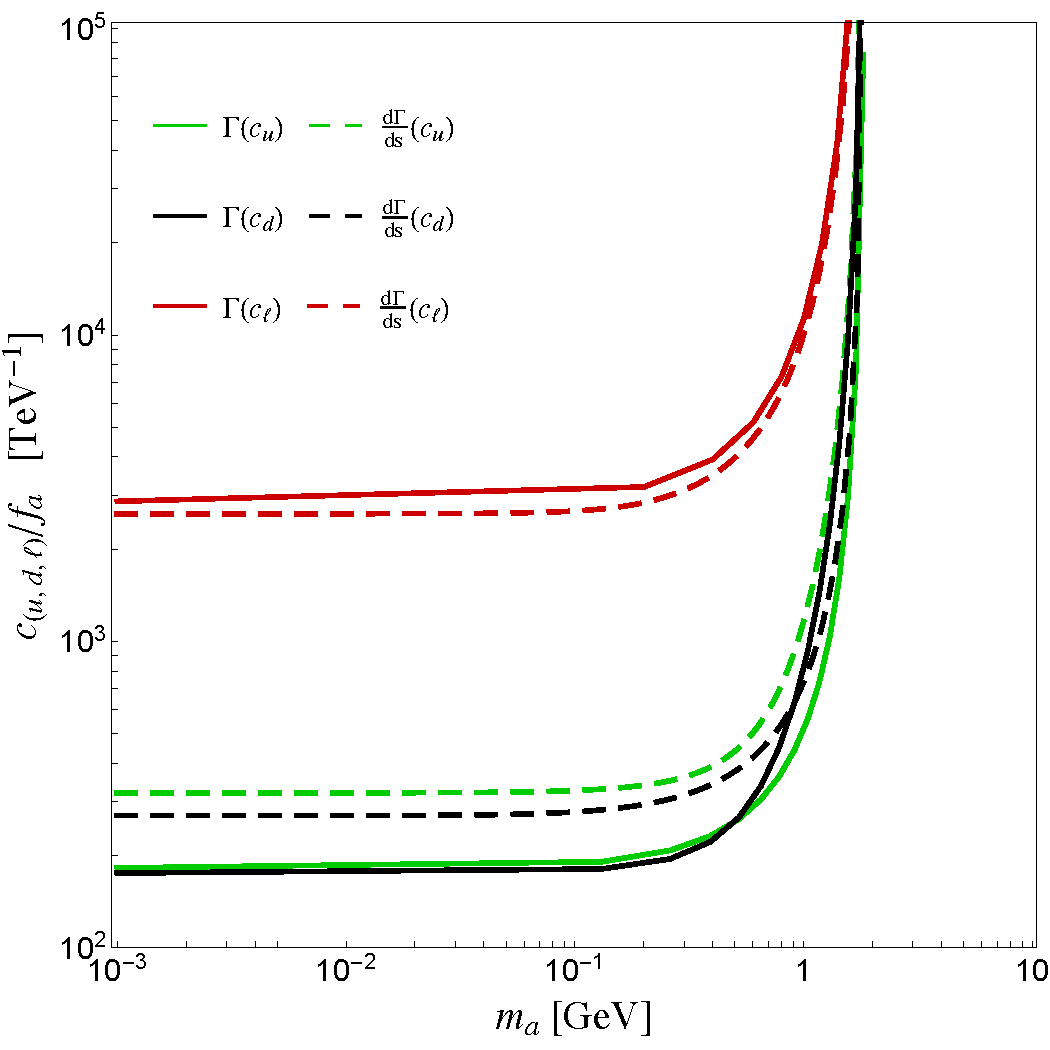
\includegraphics[width=\columnwidth]{figures/Fig3bSpro}
        \end{column}
        \begin{column}{0.5\textwidth}
            \begin{itemize}
                \item No clear improvement compared to using the complete BR.
                \item More detailed experimental data would be needed.

            \end{itemize}
        \end{column}
    \end{columns}
\end{frame}

\begin{frame}\frametitle{ALPs: Conclusions}
    \begin{itemize}
        \item We have calculated the amplitudes for $M\to \ell \nu a$ decays for generic ALP mass and couplings.
        \item We have found an improvement of a factor 10 in the couplings to quarks in these decays.
              \begin{itemize}
                  \item Most of the channels, except $K\to e\nu_e$, are not competitive with other processes.
              \end{itemize}
        \item We have obtained the most stringent limit for ALP-lepton couplings in the (sub)-GeV range.
              \begin{itemize}
                  \item Best bounds for muons ($D_S$ and $B$ decays) and electrons ($K$ decays).
              \end{itemize}
        \item We have tried using the differential distribution of 2-body vs 3-body decays, but more experimental data is needed.
    \end{itemize}
\end{frame}

\begin{frame}[plain]
    \vspace{1.3cm}
\begin{block}{\huge Summary and Conclusions}
        Chapter 9
    \end{block}
    \vspace{1.3cm}
    \begin{itemize}
\item Summary and Conclusions
\item Resumen y Conclusiones
    \end{itemize}

\end{frame}

\begin{frame}\frametitle{Summary and Conclusions}
    \begin{itemize}
\item We have performed an analysis to the $R_{K^{(*)}}$ observables, $\Delta M_S$ and $A_{CP}^\mathrm{mix}$ in the context of $Z'$ and $S_3$ leptoquarks with complex couplings, obtaining an slightly improved fit compared to the real case.
        \item After the 2019 SM prediction for $\Delta M_S$, we can assume real Wilson coefficients.
        \item We have studied global fits to the Wilson coefficients $C_{\ell q(1)}^{ii33}$ and $C_{\ell q(3)}^{ii33}$, concluding that maximal violation of Lepton Flavour Universality between the first and second generations is required by the $R_{K^{(*)}}$ anomaly, and that contributions to the $\tau$ sector improve the prediction for the $R_{D^{(*)}}$ anomaly.
        \item We have shown that future measurements in the linear electron colliders will significantly improve the constrains to lepton-universal NP contributions.
    \end{itemize}

\end{frame}

\begin{frame}\frametitle{Summary and Conclusions}
    \begin{itemize}
\item We have analyzed a proposal where the New Physics only affects the third generation in the interaction basis. When we rotate to the mass basis, we have found that the mixing to the first generation of leptons is necessary to describe the $R_{K^{(*)}}$ anomaly, since the mixing to the second generation (muons) is heavily constrained by LFV observables. In this proposal, we have identified an interesting correlation between $R_D$ and $\mathrm{BR}(B\to K \nu \bar{\nu})$.
        \item  Our work marks a novel approach to the study of the flavour anomalies, with a Machine Learning analysis being used to extract confidence intervals and correlations
              between observables. We have shown that the Machine Learning techniques constitute a suitable and useful tool for this kind of analyses.
        \item We have presented an analysis of invisible ALP production in $M\to \ell \nu a$ decays. The bounds obtained for the couplings of leptons to ALPs in the mass range of MeV-GeV are the most stringent to date.
    \end{itemize}
\end{frame}

\begin{frame}\frametitle{Summary and Conclusions}

Key points:

\vspace{0.5cm}

    \begin{itemize}
        \item Use of Effective Field Theories to describe deviations from Standard Model.
        \item Need for Global analyses in order to account for all possible effects of the New Physics.
        \item Machine Learning techniques can help in phenomenological studies.
    \end{itemize}
\end{frame}

\begin{frame}\frametitle{Summary}
    \scriptsize
    In the last years there has been a growing interest in the study of
    deviations from the predictions of the Standard Model of particle
    physics in the context of Flavour Physics. This dissertation is devoted
    to the study of these deviations, with special focus on those involving
    $B$ mesons.

    ~

    The interest on deviations from the Standard Model predictions is
    twofold: theoretical questions not yet solved and recent experimental
    measurements showing this kind of deviations. In our research we study
    two classes of these experimentally-interesting observables: the
    semileptonic decays of $B$ mesons into $K$ or $K^*$ mesons and a pair of
    charged leptons through flavour-changing neutral currents, characterized
    by the $R_{K^{(*)}}$ ratios between the muonic and the electronic branching
    ratios; and the semileptonic decays of $B$ mesons into $D$ or $D^*$ mesons, a
    charged lepton and a neutrino through flavour-changing charged currents,
    characterized by the $R_{D^{(*)}}$ ratios between the tauonic and the light
    branching ratios. We use the framework of Effective Field Theories,
    being able to obtain constraints on New Physics contributions to the
    Wilson coefficients of the effective Lagrangian from the experimental
    results. A global fit, including observables from all affected sectors,
    is considered. The sheer number of observables involved makes mandatory
    the use of numerical calculations, and in the most extreme cases, even
    using Machine Learning tools such as regression trees and SHAP (SHAPley
    Additive exPlanation) values. We use for the first time in the flavour
    context a Montecarlo analysis to extract the confidence intervals and
    correlations between observables, showing that it constitutes a suitable
    strategy to use in this kind of analysis.

    ~

    We have also extrapolated our results to specific models of New Physics;
    leptoquarks and $Z'$ bosons. We have also performed a more in-deep
    analysis of a model for Axion-Like Particles, pseudoscalars that could
    appear as pseudo-Nambu-Goldstone bosons for new global $U(1)$ symmetries.
    Unlike the traditional approaches, we have examined the case where the
    Axion-Like Particles have a non-trivial flavour structure in their
    couplings to quarks and leptons.
\end{frame}

\begin{frame}\frametitle{Resumen y Conclusiones}
    \begin{itemize}
        \item Hemos realizado un análisis de los observables $R_{K^{(*)}}$, $\Delta M_S$ y $A_{CP}^\mathrm{mix}$ en el contexto de $Z'$ y leptoquarks $S_3$ con acoplamientos complejos, obteniendo un ajuste ligeramente mejor que en el caso real.
        \item Tras la predicción de $\Delta M_S$ en el SM actualizada en 2019, podemos asumir que los coeficientes de Wilson sean reales.
        \item Hemos estudiado ajustes globales a los coeficientes de Wilson $C_{\ell q(1)}^{ii33}$ y $C_{\ell q (3)}^{ii33}$, y hemos concluido que la anomalía en $R_{K^{(*)}}$ requiere una violación máxima de la universalidad del sabor leptónico entre las dos primeras generaciones, y que las contribuciones en el sector $\tau$ pueden mejorar la predicción de $R_{D^{(*)}}$.
        \item Hemos mostrado que los futuros experimentos en colisionadores lineales de electrones mejorarán significativamente los límites experimentales a las contribuciones de Nueva Física con universalidad del sabor leptónico.
    \end{itemize}
\end{frame}

\begin{frame}\frametitle{Resumen y Conclusiones}
    \begin{itemize}
        \item Hemos analizado una propuesta en la cual la Nueva Física solo afecta a la tercera generación en la base de interacción. Al rotar a la base de masa, hemos concluido que la mezcla con la primera generación es necesaria para describir la anomalía de $R_{K^{(*)}}$, ya que la mezcla con la segunda generación (muones) está muy limitada por los observables de violación del sabor leptónico. Con esta propuesta, hemos identificado una correlación entre $R_D$ y $\mathrm{BR}(B\to K\nu\bar{\nu})$ que puede ser interesante experimentalmente.
        \item Una novedad relevante de nuestro trabajo es que utilizamos por primera vez en el contexto de las anomalías de sabor un análisis de \textit{Machine-Learning} para extraer los intervalos de confianza y las correlaciones entre observables, demostrando que es una herramienta útil y adecuada en este tipo de análisis.
        \item Hemos presentado un análisis de la producción de ALPs invisibles en las desintegraciones $M\to \ell \nu a$. Los límites obtenidos para los acoplamientos de leptones con ALPs en el rango de masas de MeV-GeV son los más estrictos hasta la fecha.
    \end{itemize}
\end{frame}

\begin{frame}\frametitle{Resumen y Conclusiones}

    Ideas clave:

    \vspace{0.5cm}

    \begin{itemize}
        \item Utilidad de las Teorías de Campos Efectivas para describir desviaciones respecto al Modelo Estándar.
\item Necesidad de realizar análisis globales para tener en cuenta todos los efectos posibles de la Nueva Física.
\item Aplicación y utilidad de técnicas de \textit{Machine Learning} en los estudios fenomenológicos.
\end{itemize}
\end{frame}

\appendix

\begin{frame}[plain, noframenumbering]
    \begin{center}
        {\huge \color{unizarblue} Thank you\\ for your attention}
    \end{center}
\end{frame}

\begin{frame}[plain, noframenumbering]
    \begin{block}{\huge Backup slides}

    \end{block}
\end{frame}

\begin{frame}
    \frametitle{$B$-meson Observables in EFT}

    
    We obtained the analytical expression for the $R_{K^{(*)}}$ observables  defined at $\mu = m_b$ as
    {\scriptsize \begin{equation*}
    R_{K^*}^{[1.1,6]} \simeq \frac{0.9875+0.1759\, \mathrm{Re}\,C_9^\mu - 0.2954\,  \mathrm{Re}\, C_{10}^\mu + 0.0212|C_{9}^\mu|^2 + 0.0350 |C_{10}^\mu|^2}{1\,\  \ \ \ \ +0.1760\, \mathrm{Re}\,C_9^e - 0.3013\, \mathrm{Re}\,  C_{10}^e + 0.0212|C_9^e|^2 + 0.0357 |C_{10}^e|^2}\ .
    \end{equation*}}
    
    We performed a fit to the WET operators
    
    \includegraphics[width=0.39\textwidth]{figures/fitre}
    \includegraphics[width=0.39\textwidth]{figures/fitIm_C9C10.pdf}\\
    
    
    
    $$R_{D^{(*)}}^\ell = R_{D^{(*)}}^{\ell, \mathrm{SM}} \frac{|1+ C_{VL}^\tau|^2}{ (|1+C_{VL}^e|^2 + |1+C_{VL}^\mu|^2)/2}\ .$$
    \end{frame}

\frame{
    \frametitle{Fits to complex Wilson coefficients (I)}
    \begin{table}
        \caption{Best fit Wilson coefficients complex values to semi-leptonic decay observables
            $R_{K^+}, R_{K^*}, P_4'$ and $P_5'$ (all available bins), allowing only one free coefficient at a
            time. Shown are also the corresponding pulls. }
        \centering
        \begin{tabular}{|c|c|c|c|c|}\hline
            & Best fit(s)      & Pull ($\sqrt{\Delta\chi^2}$) & Pull ($\sigma$)                & $\chi^2/\mathrm{d.o.f.}$ \\\hline
            $C_9^{\mu\,\mathrm{NP}}$                                               & $-1.11-0.02\;i$  & 5.94                         & 5.60 $\sigma$                  & 1.35                     \\\hline
            \multirow{2}{*}{$C_{10}^{\mu\,\mathrm{NP}}$}                            & $1.66+1.99\;i$   & \multirow{2}{*}{5.02}        & \multirow{2}{*}{4.65 $\sigma$} & \multirow{2}{*}{1.62}    \\ & $1.67-2.01\;i$ & & & \\\hline
            \multirow{2}{*}{$C_9^{\mu\,\mathrm{NP}} = -C_{10}^{\mu\,\mathrm{NP}}$} & $-1.16+1.14\;i$  & \multirow{2}{*}{6.06}        & \multirow{2}{*}{5.72 $\sigma$} & \multirow{2}{*}{1.31}    \\ & $-1.18-1.18\;i$ & & & \\\hline
            $C_9^{'\,\mu\,\mathrm{NP}}$                                            & $-0.24-0.003\;i$ & 1.07                         & 0.57 $\sigma$                  & 2.27                     \\\hline
            $C_{10}^{'\,\mu\,\mathrm{NP}}$                                         & $0.33-0.014\;i$  & 2.22                         & 1.72 $\sigma$                  & 2.17                     \\\hline
        \end{tabular}
    \end{table}
}

\frame{
    \frametitle{Fits to complex Wilson coefficients (II)}
    \begin{table}
        \caption{Best fit Wilson coefficients complex values to semi-leptonic decay observables
            $R_{K^+}, R_{K^*}, P_4'$ and $P_5'$ (all available bins), allowing only one free coefficient at a
            time. Shown are also the corresponding pulls. }
        \label{tableWC2}
        \centering
        \begin{tabular}{|c|c|c|c|c|}\hline
                                                                               & Best fit(s)     & Pull ($\sqrt{\Delta\chi^2}$) & Pull ($\sigma$)                & $\chi^2/\mathrm{d.o.f.}$ \\\hline
            \multirow{2}{*}{$C_9^{e\,\mathrm{NP}}$}                            & $-3.29+5.02\;i$ & \multirow{2}{*}{4.85}        & \multirow{2}{*}{4.47 $\sigma$} & \multirow{2}{*}{1.67}    \\ & $-3.35-5.04\;i$ & & & \\\hline
            \multirow{2}{*}{$C_{10}^{e\,\mathrm{NP}}$}                         & $-0.27+3.48\;i$ & \multirow{2}{*}{4.72}        & \multirow{2}{*}{4.34 $\sigma$} & \multirow{2}{*}{1.70}    \\ &  $-0.27-3.48\;i$ & & & \\\hline
            \multirow{2}{*}{$C_9^{e\,\mathrm{NP}} = -C_{10}^{e\,\mathrm{NP}}$} & $-3.29+4.58\;i$ & \multirow{2}{*}{4.85}        & \multirow{2}{*}{4.47 $\sigma$} & \multirow{2}{*}{1.67}    \\ & $-3.35-4.59\;i$ & & & \\\hline
            \multirow{2}{*}{$C_9^{'\,e\,\mathrm{NP}}$}                         & $-0.59+3.89\;i$ & \multirow{2}{*}{4.81}        & \multirow{2}{*}{4.43 $\sigma$} & \multirow{2}{*}{1.68}    \\ & $-0.59-3.89\;i$ & & & \\\hline
            \multirow{2}{*}{$C_{10}^{'\,\mu\,\mathrm{NP}}$}                    & $0.52+3.88\;i$  & \multirow{2}{*}{4.81}        & \multirow{2}{*}{4.43 $\sigma$} & \multirow{2}{*}{1.68}    \\ & $0.53-3.88\;i$ & & &  \\\hline
        \end{tabular}
    \end{table}
}

\frame{
    \frametitle{Observables in the $Z'$ model}
    \section{Model dependant}
    \begin{table}
        \caption{Best fits, and corresponding pulls, to $R_{K^+}, R_{K^*}, \Delta M_s$
            and $A_{CP}^\mathrm{mix}$; considering real,
            imaginary and complex Wilson coefficients on the $Z^{'}$
            model.}
        \label{tableZ}
        \centering
        \begin{tabular}{|c|c|c|c|}\hline
            Best fits                     & Real                           & Imaginary                   & Complex                      \\\hline
            $\lambda_{23}^{Q}$            & $-0.002 $                      & $\pm 0.047\;i$              & $-0.0020-0.0021\;i$          \\\hline
            $M_{Z'}$                      & 1.31  TeV                      & 12  TeV                     & 1.08  TeV                    \\\hline
            Pull ($\sqrt{\Delta \chi^2}$) & 5.70                           & 1.61                        & 6.05                         \\\hline
            Pull ($\sigma$)               & 5.39 $\sigma$                  & 1.09 $\sigma$               & 5.43 $\sigma$                \\\hline
            $\chi^2/\mathrm{d.o.f}$       & 1.41                           & 2.12                        & 1.34                         \\\hline
            $R_{K^+}$                     & $0.66 \pm 0.05$                & $ 1.00 \pm 0.01 $           & $0.65 \pm 0.07 $             \\\hline
            $R_{K^*}^{[0.045,1.1]}$       & $0.849 \pm 0.013$              & $ 0.93 \pm 0.02$            & $ 0.84\pm 0.02$              \\\hline
            $R_{K^*}^{[1.1, 6]}$          & $0.68 \pm 0.05$                & $1.00 \pm 0.01$             & $ 0.68\pm 0.07$              \\\hline
            $\Delta M_s$                  & $ 20.41 \pm 1.26 $ ps${}^{-1}$ & $18.0 \pm 1.7 $ ps${}^{-1}$ & $ 19.95\pm 1.27$ ps${}^{-1}$ \\\hline
            $A_{CP}^\mathrm{mix}$         & $-0.0369 \pm 0.0002$           & $ -0.041 \pm 0.002 $        & $-0.035 \pm 0.003$           \\\hline
        \end{tabular}
    \end{table}
}

\frame{
    \frametitle{Observables in the $S_3$ model}
    \begin{table}
        \caption{Best fits, and corresponding pulls, to $R_{K^+}, R_{K^*}, \Delta M_s$
            and $A_{CP}^\mathrm{mix}$; considering real,
            imaginary and complex Wilson coefficients on the $S_3$ leptoquark.}
        \label{tableLQ}
        \centering
        \begin{tabular}{|c|c|c|c|}\hline
            Best fits                     & Real                         & Imaginary                  & Complex                    \\\hline
            $y^{QL}_{32} y^{QL*}_{22}$    & $0.04 $                      & $ -1.67\;i$                & $0.033+0.034\;i$           \\\hline
            $M_{S_3}$                     & 5.19  TeV                    & 50  TeV                    & 4.10  TeV                  \\\hline
            Pull ($\sqrt{\Delta \chi^2}$) & 5.82                         & 1.10                       & 5.90                       \\\hline
            Pull ($\sigma$)               & 5.47 $\sigma$                & 0.60 $\sigma$              & 5.27 $\sigma$              \\\hline
            $\chi^2/\mathrm{d.o.f}$       & 1.38                         & 2.16                       & 1.39                       \\\hline
            $R_{K^+}$                     & $0.64 \pm 0.06$              & $1.00 \pm 0.01$            & $0.62 \pm 0.14$            \\\hline
            $R_{K^*}^{[0.045,1.1]}$       & $0.835 \pm 0.015$            & $ 0.93\pm 0.02 $           & $0.84 \pm 0.04$            \\\hline
            $R_{K^*}^{[1.1, 6]}$          & $ 0.66 \pm 0.06$             & $1.00 \pm 0.01$            & $0.66 \pm 0.14$            \\\hline
            $\Delta M_s$                  & $20.07 \pm 1.27$ ps${}^{-1}$ & $18.8 \pm 1.7$ ps${}^{-1}$ & $20.0 \pm 1.2$ ps${}^{-1}$ \\\hline
            $A_{CP}^\mathrm{mix}$         & $-0.0374 \pm 0.0006$         & $ -0.039 \pm 0.002$        & $-0.032 \pm 0.003$         \\\hline
        \end{tabular}
    \end{table}

}

\begin{frame}\frametitle{SMEFT Fits: Scenarios}
    
    \begin{table}
        \centering \scriptsize \hspace{-1cm}
        \begin{tabular}{|c|c|c|c|c|c|c|c|}\hline
      \multicolumn{2}{|c|}{\multirow{2}*{Scenario}}&\multirow{2}*{$C_{\ell
          q}^e$} &\multirow{2}*{$C_{\ell q}^\mu$}&\multirow{2}*{$C_{\ell
          q}^\tau$} &\multirow{2}*{$\Delta\chi^2_\mathrm{SM}$} & Pull & Pull
      \\ \multicolumn{2}{|c|}{} & & & & & from SM & to VII\\\hline
      I& $e$	& $-0.15 \pm 0.04$ & & & 8.19 &	$2.86\,\sigma$ & $4.07\,\sigma$\\\hline
      II& $\mu$ & & $0.15 \pm 0.03$ & & 17.89 & $4.23\,\sigma$ & $2.75\,\sigma$\\\hline
      III& $\tau$ & & & $-0.30\pm 0.19$ & 2.55 & $1.60\,\sigma$ & $4.68\,\sigma$\\\hline
      IV& $e$ and $\mu$ & $-0.15 \pm 0.09$ &	$0.15 \pm 0.06$	& & 26.10 & $4.73\,\sigma$ & $1.42\,\sigma$\\\hline
      V& $e$ and $\tau$ & $-0.15 \pm 0.06$ & & $-0.3 \pm 0.3$ & 10.68 & $2.82\,\sigma$ & $4.18\,\sigma$\\\hline
      VI& $\mu$ and $\tau$ &	& $0.15 \pm 0.05$ & $-0.3 \pm 0.3$ & 19.96 & $4.07\,\sigma$ & $2.86\,\sigma$\\\hline
      VII& $e$, $\mu$ and $\tau$ & $-0.15 \pm 0.11$ & $0.15 \pm 0.07$ &
      $-0.3 \pm 0.3$ & 28.12 & $4.64\,\sigma$ &\\\hline
      VIII& $e = \mu = \tau$	& $0.04 \pm 0.03$ & $0.04 \pm 0.03$ &
      $0.04 \pm 0.03$ & 1.98 & $1.40\,\sigma$ & $4.74\,\sigma$\\\hline
      IX& $e = -\mu = \tau$ & $-0.152\pm0.005$ & $0.152\pm0.005$ &
      $-0.152\pm0.005$ & 27.73 & $5.27\,\sigma$ & $0.62\,\sigma$\\\hline
      X & $e = -\mu$ & $-0.15\pm 0.03$ & $0.15\pm 0.03$ & & 26.10 & $4.94\,\sigma$ & $1.42\,\sigma$\\\hline
      XI & $e = -\mu$, $\tau$ & $-0.15 \pm 0.05$ & $0.15\pm0.05$ & $-0.3 \pm 0.3 $ & 28.12 & $4.94\,\sigma$ & $0\,\sigma$ \\\hline
        \end{tabular}
      \end{table}
\end{frame}

\begin{frame}
    \frametitle{Electron colliders and Flavour Physics}
    Electron colliders are powerful tools in testing neutral currents:
    \begin{itemize}
    \item Clean signatures.
    \item Small uncertainties.
    \item Detailed differential analyses in di-fermion final states.
    \item Different longitudinal polarisation of the beams.
    \item Experimental sensitivity increases with $\sqrt{s}$,
    $$\mathcal{A}_\mathrm{dim 6} \sim C \frac{E^2}{\Lambda^2}.$$
    \end{itemize}
\end{frame}
    
\begin{frame}
    \frametitle{Probing Wilson coefficients}
    \begin{itemize}
    \item ILC at $\sqrt{s} = 250 \mathrm{GeV}$ has better sensitivity than HL-LHC.
    \item ILC at $\sqrt{s} = 1000 \mathrm{GeV}$ can probe up to $\Lambda \sim 100 \mathrm{TeV}$.
    \end{itemize}
    \begin{center}
    \includegraphics[width=0.9\textwidth]{figures/operators_esu}\\
    \colorcite{R. K. Ellis \textit{et al.} arXiv:1910.11775 [hep-ex]}
    \end{center}
    $$\mathrm{EOM}\left\{ \begin{matrix}
    {\color[HTML]{4285f4} \mathcal{O}_{2W}} \Leftrightarrow \mathcal{O}_{\ell q(3)}\\ {\color[HTML]{ff9900} \mathcal{O}_{2B}} \Leftrightarrow \mathcal{O}_{\ell q(1)}
    \end{matrix} \right.  $$
\end{frame}

\begin{frame}
        \frametitle{Electroweak precission tests}
        ILC can improve the precission of EW observables that enter in the global fit, both in Giga-$Z$ configuration and at $\sqrt{s} = 250 \mathrm{GeV}$.
        \begin{center}
        \includegraphics[width=0.75\textwidth]{figures/EWPO}\\
        \colorcite{R. K. Ellis \textit{et al.} arXiv:1910.11775 [hep-ex]}
        \end{center}
\end{frame}
        
        

\begin{frame}\frametitle{ML Fit: Matching and $R_{K^{(*)}}$}
    Translating between the two EFTs: 1-loop RG running $\Lambda \to \mu_\mathrm{EW}$ + matching:
    \begin{itemize}
        \item {\small $C_9^\ell \approx \frac{\sqrt{2}}{V_{tb}V_{ts}^* G_F \Lambda^2}\left[ \frac{2\pi^2}{e^2}(C_{\ell q(1)}^{\ell\ell23}+C_{\ell q(3)}^{\ell\ell23}) + \textcolor{blue}{\frac{\log(m_b/\Lambda)}{3}(C_{\ell q(1)}^{3323}+C_{\ell q(3)}^{3323})}\right]\, $.}
        \item {\small $C_{10}^\ell \approx \frac{-\sqrt{2}}{V_{tb}V_{ts}^* G_F \Lambda^2} \frac{2\pi^2}{e^2}(C_{\ell q(1)}^{\ell\ell23}+C_{\ell q(3)}^{\ell\ell23}) \, $.}
        \item {\small $C_{VL}^\ell \approx \frac{-1}{\sqrt{2}G_F\Lambda^2}\left(C_{\ell q(3)}^{\ell\ell33}+ \frac{V_{cs}}{V_{cb}}C_{\ell q(3)}^{\ell\ell 23}\right)$\,.}
        \item {\small $C_\nu^\ell \approx \frac{\sqrt{2}}{e^2 V_{tb}V_{ts}^* G_F \Lambda^2}\left[2\pi^2(C_{\ell q(1)}^{\ell\ell 23}-C_{\ell q(3)}^{\ell\ell 23})+\textcolor{blue}{\frac{2{g'}^2}{3}\log(m_b/\Lambda)C_{\ell q(3)}^{\ell\ell 23}}\right]\,$.}
    \end{itemize}

    \textcolor{blue}{Loop-level corrections} break the relation $C_9^\ell = -C_{10}^\ell$.

    ~

    $R_{K^{(*)}}$ requires mixing with the first generation ($\alpha^\ell$):
    \begin{align*}
        C_9^e   & = -C_{10}^e + C_9^\mathrm{loop} = -0.32\,, \qquad\qquad                 &  & C_{10}^e =-0.36\,,             \\
        C_9^\mu & = {\color{gray}-C_{10}^\mu} + C_9^\mathrm{loop} = -0.67\,, \qquad\qquad &  & {\color{gray}C_{10}^\mu =0}\,.
    \end{align*}

\end{frame}

\begin{frame}\frametitle{ML Fit: Correlations between WCs}

\begin{columns}[onlytextwidth]
\begin{column}{0.6\textwidth}
    \includegraphics[width=\columnwidth,clip]{figures/coeffcorr.pdf}

\end{column}
\begin{column}{0.4\textwidth}
\begin{itemize}
    \item Correlation in $C_{10}^e$, $C_{VL}^e$ and $C_\nu^e$, all proportional to $C \lambda^q_{23} \lambda^\ell_{11}$.
    \item Correlation in $C_{10}^\mu$, $C_{VL}^\mu$ and $C_\nu^\mu$, all proportional to $C \lambda^q_{23} \lambda^\ell_{22}$.
    \item Correlation in $C_{VL}^\tau$ and $C_\nu^\tau$, all proportional to $C \lambda^q_{23} \lambda^\ell_{33}$.
    \item $C_9^\mu = C_9^\mathrm{loop}$ correlated to $\tau$ sector ($C\lambda^q_{23} \approx C\lambda^q_{23} \lambda^\ell_{33}$).
    \item $C_9^e = -C_{10}^e + C_9^\mathrm{loop}$ partially correlated to $e$ and $\tau$ sectors.
\end{itemize}

\end{column}
\end{columns}
\end{frame}

\begin{frame}\frametitle{ML Fit: Likelihood and SHAPs}

\begin{center}
    \includegraphics[width=0.45\textwidth]{figures/evoplot_betal.pdf}
    \includegraphics[width=0.45\textwidth]{figures/evoplot_alphaq.pdf}   \end{center}
\begin{center}
    \includegraphics[width=0.45\textwidth]{figures/SHAP_bl.pdf}
    \includegraphics[width=0.45\textwidth]{figures/SHAP_aq.pdf}
\end{center}

\end{frame}

\begin{frame}\frametitle{ALPs: Hadronic amplitude and differential distribution}The functions $\Phi^{(q,Q)}_M (m_a^2)$ contain the integrals over the quark momentum fraction
    and are defined respectively as:
    \begin{align*}
        \Phi^{(q)}_M (m_a^2) & = \int^{1-\delta_M}_0 \frac{p_a \cdot P_M}{m_a^2-2\,(1-x)\,p_a\cdot P_M} \, \phi_M(x) \,g_M(x)\, dx\,, \\
        \Phi^{(Q)}_M (m_a^2) & = \int^1_{\delta_M} \frac{p_a \cdot P_M}{m_a^2-2\,x\,p_a\cdot P_M}     \, \phi_M(x) \,g_M(x)\, dx \,.
    \end{align*}
    The presence of the kinematical cutoff $\delta_M=m_a/(2 M_M)$ prevents the appearance of unphysical bare singularities.

    ~

    The differential decay rate in the rest frame of the meson
    $$\left(d \Gamma_M \right)_{RF} = \frac{1}{(2 \pi)^3} \frac{1}{32 M_M^3} |\overline{\mathcal{M}_h} + \overline{\mathcal{M}_\ell}  |^2 \,ds \,du \,.$$

    integrated over the Mandelstam variables
    \begin{align*}
        s & = (P_M - p_\ell)^2 = (p_\nu+p_a)^2 = M_M^2 + m_\ell^2- 2 M_M \omega_\ell\,, \\
        u & = (P_M - p_a)^2 = (p_\ell+p_\nu)^2 = M_M^2 + m_a^2- 2 M_M \omega_a\,.
    \end{align*}

    The interference term is proportional to both the ALP mass and lepton mass.

\end{frame}


\end{document}